This chapter first describes the two datasets MS COCO and 3Dshapes used in this work. Then, the agents' architecture is presented. There are two agents---the speaker and the listener agents---whose architectures are shared across all experiments. Finally, the single experiments and their results are discussed.

\section{Datasets}

This work uses two datasets for the reference game. The dataset chosen for the main experiments is the MS COCO Captions dataset \parencite{chen2015microsoft}. As it is one of the most widely used image datasets containing real photos of common objects and scenes, this choice was motivated by the goal of this work is to test multi-agent communication on natural images annotated with natural language captions. 

Further, a second dataset was chosen for conducting baseline experiments in order to investigate potential sources of language drift---the 3Dshapes dataset developed by \textcite{burgess20183d}. This dataset was chosen due to its systematic content and exhaustive annotations of all relevant image features, allowing to automatically generate exhaustive natural language captions for the dataset. This dataset has by far less features and categories varying across the images compared to the main dataset, providing a baseline for estimating the models' performance in a more controlled environment.

Both datasets are used for constructing the reference game which procedes in the following way:
\begin{enumerate}
	\item A random image is sampled from the dataset as the target $t$.
	\item A second image is sampled as the distractor $d$ (either at random or following constraints; see below for details).
	\item The speaker agent $S$ recieves both images, the target image being marked, respectively. This is accomplished by always passing the target as the first image. It emits a message $m$ describing the target.
	\item The listener agent $L$ recieves both images along with the message $m$, but doesn't know which image is the target.
	\item The listener selects the target image based on the message. If the selection was correct, both agents receive a positive reward, and a negative one otherwise.	 
\end{enumerate}

The next two sections describe in detail the properties of the datasets and how they were preprocessed for the experiments.

\subsection{MS COCO}
\label{ds:coco}
The MS COCO Captions dataset \parencite{chen2015microsoft} contains images and respective annotations from the 2014 split of the MS COCO dataset \parencite{lin2014microsoft}. Figure \ref{fig:coco_example} presents an example image and annotations form the dataset. The dataset contains 82,783 images in the training split, each associated with around five human-annoated caption, resulting in a total of 414,113 unique image-caption pairs. The validation split contains 40,504 images, annotated with a total of 202,654 human-produced captions. The respective dataset splits and annotations were downloaded from \url{https://cocodataset.org/#download}.
Furthermore, each image is annotated with bounding boxes of objects and category labels for the depicted objects. There are 80 different basic-level annotation categories, listed in the Appendix \ref{appendix}. These 80 categories are grouped into 12 superordinate categories: person, accessory, indoor, appliance, food, kitchen, sports, furniture, outdoor, animal, electronic and vehicle.
On average, 2.9 basic-level categories and 2.3 superordinate categories occur per image.
\pt{There will be a table with super-basic category mappings and counts of at least each super category}.

The natural language captions associated with the images contain a total of 24,697 unique tokens. Yet over 99\% of the words occuring in the entire dataset are covered by 6000 most frequent tokens. 
The final size of the vocabulary $V$ used in the experiments is 4054, including four special tokens \texttt{START, END, UNK, PAD}, as it comprises over 98\% of the token distribution mass, while comprising 16.4\% of unique tokens occurring in all captions. This vocabulary size was chosen as a good trade-off between a sufficient variety of words that the speaker can choose to describe the images and an action space size which is still learnabale in the current set-up. 

The minimal caption length occuring in the dataset is six tokens, the maximal length is 57 tokens. The mean caption length is 11.3 tokens (based on tokenization with the basic English tokenizer provided by the \texttt{torchtext} package). Since recurrent neural networks may have issues with learning very long sequences \parencite[e. g.,][]{jaeger2002tutorial}, captions exceeding the length of 15 tokens were truncated. This cut-off length was chosen because it is the minimal length at which over 99\% of the captions didn't have to be truncated. %\pt{maybe include a density plot, side by side with the vocab count density one}
During preprocessing, the captions were lowercased, tokenized with the \texttt{torchtext} tokenizer mentioned above and mapped to numerical indices.  The resulting vocabulary is shared between the speaker and listener agents in all experiments. 

The following preprocessing steps were applied to all images before training: the images were resized to 256 pixels, random $224\times224$ pixel crops were taken, images were horizontally flipped with a probability of 0.5 in order to increase the speaker's viewpoint invariance and each RGB channel was normalized using values expected by the pretrained ResNet50 module.

For the baseline experiments, the training pairs of images were sampled at random. In contrast, for the experiment involving similar training pairs the images were sampled such that the distractor depicted objects similar to the target. This was controlled via the category annotations accompanying each image. The training pairs were constructed so that they were annotated with at least three same basic-level categories, or, in case there were less than three, if all annotated categories matched.

\subsection{3Dshapes}
\label{ds:3dshapes}
The 3Dshapes dataset introduced by \textcite{burgess20183d} contains 480.000 synthetically generated images. These images depict different three-dimensional geometric objects in abstract space, systematically varying along six different features. These features are the color of the ground on which the object resides (ten values), the color of the background walls (ten values), the color of the object itself (ten values), the type of object (four values), its size (eight values) and its position within the depicted room (15 values). %\pt{Table X depicts / describes the possible values of each dimension}. 
The $64\times64$ pixel images are labeled with six-dimensional vectors, each position representing the value of one of the six features.
The dataset was downloaded from \url{https://storage.cloud.google.com/3d-shapes/3dshapes.h5}.
%\pt{XXX images were used for training the agents in the 3Dshapes experiment, and YYY images were used for testing.}
\begin{figure}
\centering
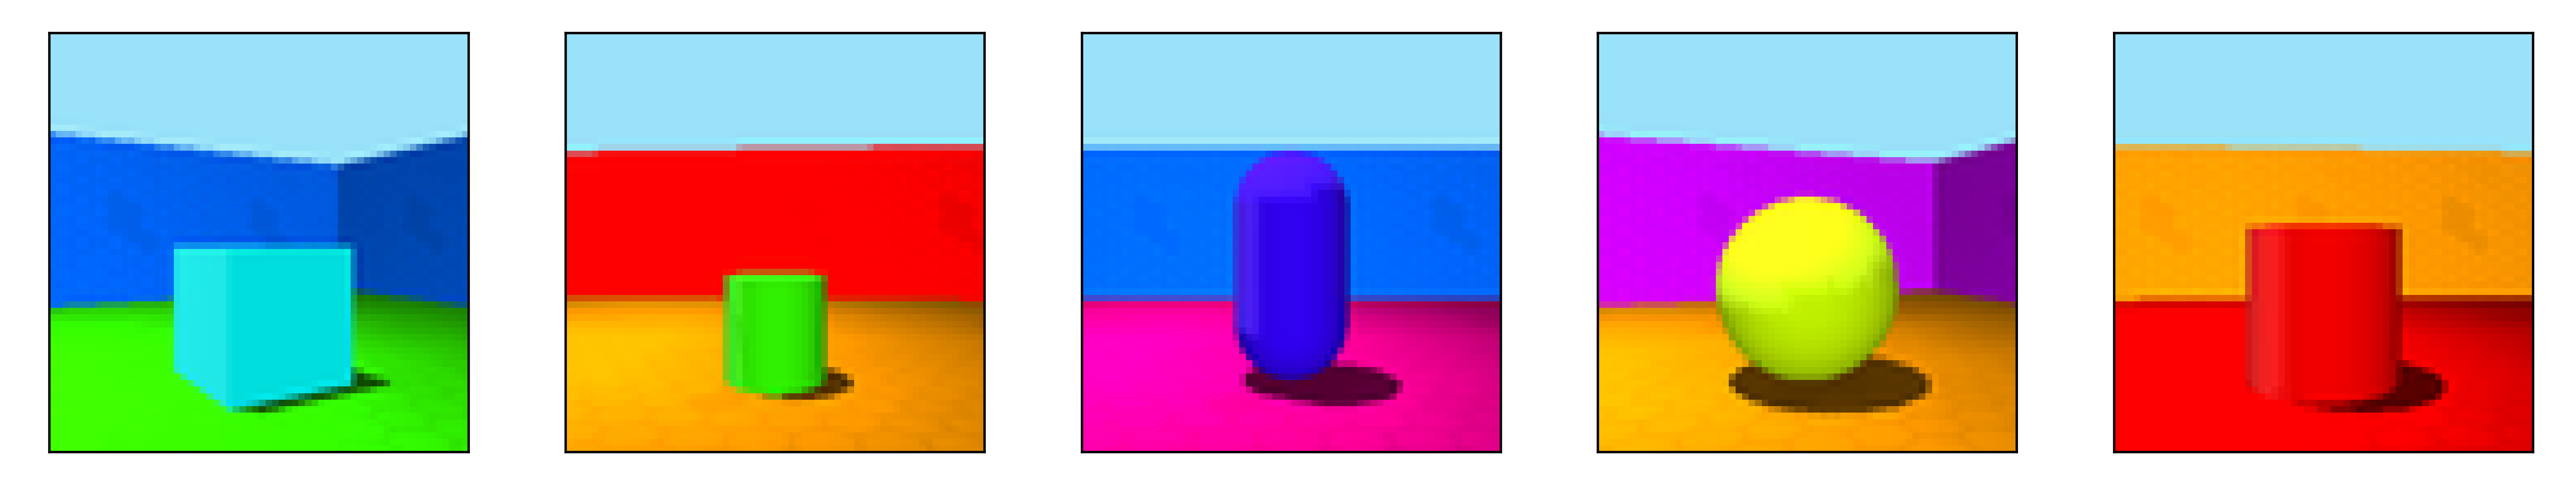
\includegraphics[width=\linewidth]{images/3dshapes_example.png}
\caption{Example images from the 3Dshapes dataset. Examples of corresponding generated captions (from left to right): ``A big cyan block in the right corner on green floor in front of a medium blue wall.''; ``The green cylinder in the middle in front of a red wall on orange floor is tiny.''; ``A middle-sized dark blue pill located in the middle in front of a medium blue wall on pink floor.''; ``The picture shows a huge yellow ball on orange floor in front of a purple wall close to the right side.''; ``The large cylinder on red floor in front of a orange wall in the middle is red.''.}
\label{fig:3dshapes_example}
\end{figure}  

\subsubsection{Caption Generation}

The dataset provides symbolic feature labels of the images. However, since the goal of presented work is training artificial agents to use natural language in communication, English captions were generated for this dataset. More specifically, two datasets were generated. 

The first dataset is tailored towards studying the effect of including maximally exhaustive image descriptions in the training data. Therefore, generated captions include natural language descriptions of all six features and their values, appearing in different syntactic constructions. Figure~\ref{fig:3dshapes_example} shows an example image along with sample generated captions. The syntactic variations were introduced in order to avoid potential effects of order in which descriptions of certain features might occur.
The captions were generated by constructing generation rules and sampling all possible resulting sentences using the \texttt{nltk} package \parencite{bird2006nltk}. The resulting dataset contains 20 synonymous captions per image, five of which are sampled at random for training in order to match the MS COCO conditions. The captions were build using a vocabulary of 49 tokens. Maximal caption length is 25 tokens, the minimal length is 16 and mean caption length is 18.9 tokens. 
%\pt{The most prominent grammatical structure in the dataset was...}

The second dataset provides the comparison for investigating the role of having exhaustive captions in the training dataset, while keeping constant the vocabulary size. That is, this dataset contains \textit{non-}exhaustive captions which only mention two to three out of six features of each image. These captions were generated using the same procedure. 27 captions per image were generated. The maximal caption length in this dataset is 13 tokens, the minimal is three tokens and the average length is 7.2 tokens.
The same examples along with nonexhaustive captions can be seen in Fig.~\ref{fig:3dshapes_example_short}.
%\pt{potential confound with length.}
The comparability of the vocabulary sizes is important in that it determines the difficulty of learning the policy with REINFORCE which represents the functional learning in these experiments \parencite[cf.][]{havrylov2017emergence}.

The generation rules and the corresponding code can be accessed under \url{https://github.com/polina-tsvilodub/3dshapes-language}.

\begin{figure}
	\centering
	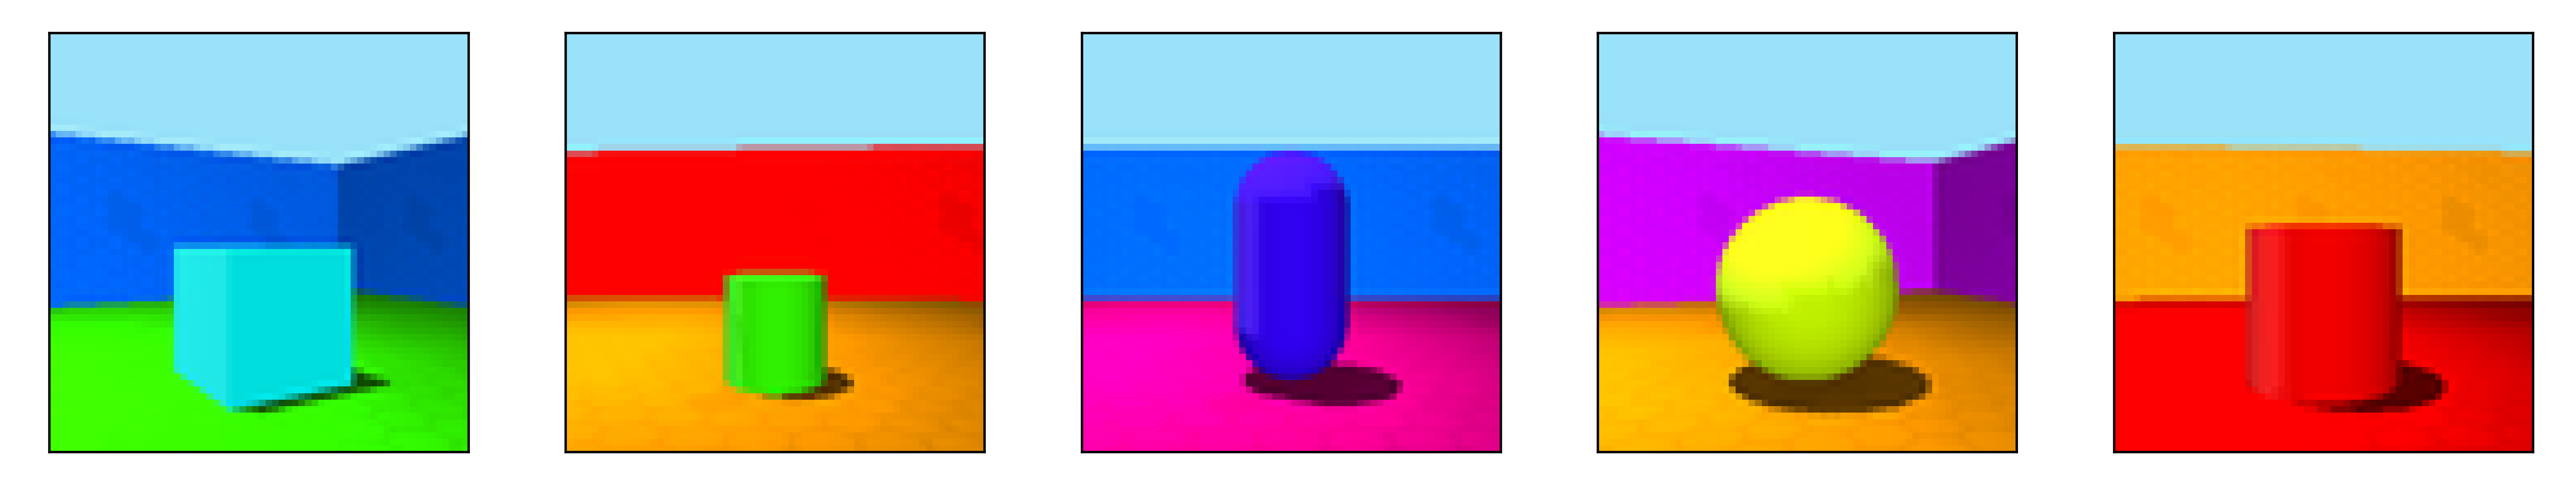
\includegraphics[width=\linewidth]{images/3dshapes_example.png}
	\caption{Example images from the 3Dshapes dataset. Examples of corresponding generated captions (from left to right): ``The block is in front of a medium blue wall.''; ``A tiny cylinder.''; ``There is a pill in the middle.''; ``A yellow ball close to the right side.''; ``A red cylinder in front of a orange wall.''.}
	\label{fig:3dshapes_example_short}
\end{figure} 
%\pt{TBD. Cite Bruni's paper with the grammar stuff.}

Akin to MS COCO experiments, baseline experiments are conducted on random target-distractor pairs. For the similar pairs experiment, the distractor is chosen so that it matches the target with respect to at least three out of six features. For instance, if the target depicts a tiny red cube in the left corner on yellow floor and with blue background, the distractor could depict a tiny blue cube in the right corner on yellow floor and with green background.

%This dataset was chosen due to the systematicity of its content , allowing to generate natural language captions for each image which would exhaustively describe all features of the images. Since no such captions exist to the author's knowldege, they are generated as part of this thesis. To this end, a base context-free grammar (CFG) containing production rules for captions was manually created. The syntactic rules were constructed on the basis of examples of captions created by the author for samples from the dataset. Each caption must contain descriptions of all six feature dimensions. The terminal production rules mapping the pre-terminal to natural language labels are chosen for each image based on its unique feature value configuration. For each image, \pt{X captions are sampled from all the possible productions allowed by the grammar}.

%\pt{Discuss aspects to be taken care of, like vocab size, caption lengths etc}.

\section{Architecture}
The architecture of the agents follows \textcite{lazaridou2020multi}, except minor details to be explained below. As described in Chapter \ref{chapter03}, \textcite{lazaridou2020multi} explore different ways to parametrize the speaker agent, and the current work replicates the ``multi-task learning'' parametrization (p. 5). This choice is motivated by the fact that among their architectures, this is the only one where the speaker agent learns to produce messages and its core image captioning capability while having access to both the target and the distractors, as opposed to models relying on sampling captions from a pretrained single-image captioning models. The chosen architecture is used in all experiments.

Both agents have two components: a visual embedding module which takes as input the target and distractor images, and a language module. More specifically, the visual module for both agents embeds image features which were extracted using the same pre-trained ResNet50 model \parencite{he2016deep}. The weights were accessed through the \texttt{torchvision.models} API \parencite{marcel2010torchvision}. Features from all training images of the dataset were extracted and saved and then retrieved when training all agents. 
The language module differs for the two agents, so details are provided below. 
The code for all experiments can be found under \url{https://github.com/polina-tsvilodub/mSc-thesis}. 

\subsection{Speaker}
The speaker receives as input tuples \texttt{(targets, distractors)}, where \texttt{targets} as well as \texttt{distractors} are features extracted from the ResNet50 for the sampled pairs, respectively. That is, the speaker knows which of the the two images in a given iteration of the reference game is the target for which the message should be produced. The speaker then produces a probability distribution over vocabulary tokens of the message given the input $P(m \mid i_t, i_d)$, parametrized by the speaker model parameters $\theta_S$. From a reinforcement learning perspective, training the speaker amounts to estimating the parametrized speaker policy $\pi_{\theta_s}(m \mid i_t, i_d)$.

The speaker model consists of a linear layer which projects the 2048-dimensional image features to 512-dimensional embedding space. The linear layer is first applied to both the target images and then to the distractors, resulting in embeddings $i_t$ and $i_d$, respectively. The vectors are concatenated to $[i_t; i_d]$, the target embeddings always being the first ones, such that the speaker network implicitly knows which features represent the target. These 1024-dimensional vectors are used as additional context in the speaker's language module. The core of the module is the recurrent Long Short-Term Memory (LSTM) cell \parencite{hochreiter1997long}. More specifically, the language module consists of three layers: an embedding layer, mapping the vocabulary to 512-dimensional word embeddings, a one-layer LSTM with 512-dimensional hidden and cell states; and a linear layer on top, mapping the last hidden state of the LSTM to a distribution over the vocabulary. The size of the vocabulary depends on the dataset (see above).

During the reference game training, the speaker receives pairs of images, embeds them and prepends the concatenated embedding to the special \texttt{START} token. This 1536-dimensional embedding is then passed through the LSTM and the linear output layer. The next token is sampled from a categorical distribution parametrized with the probabilities computed from the hidden state in the previous timestep. The sampled token is concatenated with the image embeddings and input to the next timestep. This procedure repeats until the \texttt{END} token is sampled or the maximum caption length is achieved. The \textit{baseline} experiments use the pure decoding strategy; additional experiments investigate the effects of using greedy decoding (see Chapter \ref{chapter02}). This architecture is also a common practice in image captioning literature (cf. Chapter \ref{chapter02}). Another possible approach that could be explored in future work would be to initialize the hidden states of the LSTM with the visual embeddings. In this case, the hidden and cell states of the LSTM were initialized with random values sampled from the standard normal distribution.The embedding and last linear layers' weights were initialized with random values sampled from the uniform distribution between -0.1 and 0.1, the biases were initialized with zeroes.  
This architecure results in a total of \pt{10,429,910 check} trainable parameters.  %\pt{Make a graphic of the models and / or the reference game}.

\subsection{Listener}
The listener receives as input the tuples \texttt{(images1, images2, messages)}, the first two inputs being ResNet50 features of the image pairs, input in random order, such that the agent doesn't know which image is the target. The \texttt{message} is the caption produced by the speaker. The listener then produces scores $P(i|m)$ over images identifying which one is the target, parametrized by the listener model parameters $\theta_L$.

The message is passed to the language module which consists of an embedding layer, mapping the vocabulary to 512-dimensional word embeddings, and a one-layer LSTM with 512-dimensional hidden and cell states. All weights are initialized analagously to the respective weights of the speaker model. The hidden cell state $h_i$ at the last time step of embedding the received message is used as the final message representation. 
The visual module of the listener consists of a linear layer which also projects the 2048-dimensional image features to a 512-dimensional embedding space. The images are passed through the linear layer one after the other, resulting in embeddings $i_1$ and $i_2$. Finally, the listener computes the dot products between each image embedding and the message embedding. The target is sampled from a categorical distribution parametrized with probabilities computed based on the dot products.  
The architecture results in \pt{check 1,049,088} trainable parameters for the listener's visual module and \pt{check 4,176,896} trainable parameters for its LSTM.

%\pt{listener policies.}

\subsection{General Training Details}

All experiments were trained with a batch size of 64 pairs, using the Adam optimizer with a learning rate  of 0.001 \parencite{kingma2014adam}. In the reference game setting, due to computational constraints, the models were trained for two epochs per experiment. \footnote{All experiments were conducted on a MacBook Pro with four Intel cores i7-1068NG7 with CPU @ 2.30GHz. On average, pretraining took 2h/epoch, reference games took 6h/epoch.} 

In the reference games, the speaker parameters $\theta_S$ were updated by optimizing a compound loss function $J_s$. More precisely, the speaker loss consisted of a weighted sum of a functional loss $L_f$ and a structural loss $L_s$. The former was computed via the REINFORCE rule based on the listener's task performance (i.e., referential success). The speaker received the reward 1 if the listener guessed the target successfully, and -1 otherwise. The latter was computed via cross-entropy between the message produced by the speaker and the ground truth caption for the given target image. $L_f$ additionally included an entropy regularization term, weighted by 0.1. The resulting loss is $J_s = (1-\lambda_s)L_f + \lambda_s L_s$. 
The listener parameters $\theta_L$ were updated via cross-entropy loss $J_l$ optimized based on the guessed target classification of the images and the ground truth targets using cross-entropy loss. 


\section{Experiment Procedures and Results}

%\pt{when discussing results and esp PPL, \cite{havrylov2017emergence} also compute encoder PPLs}

This section provides an overview of conducted experiments and discusses their procedures as well as results.

\subsection{Speaker Pretraining}
\label{speaker_pretraining}
\begin{figure}
	\centering
	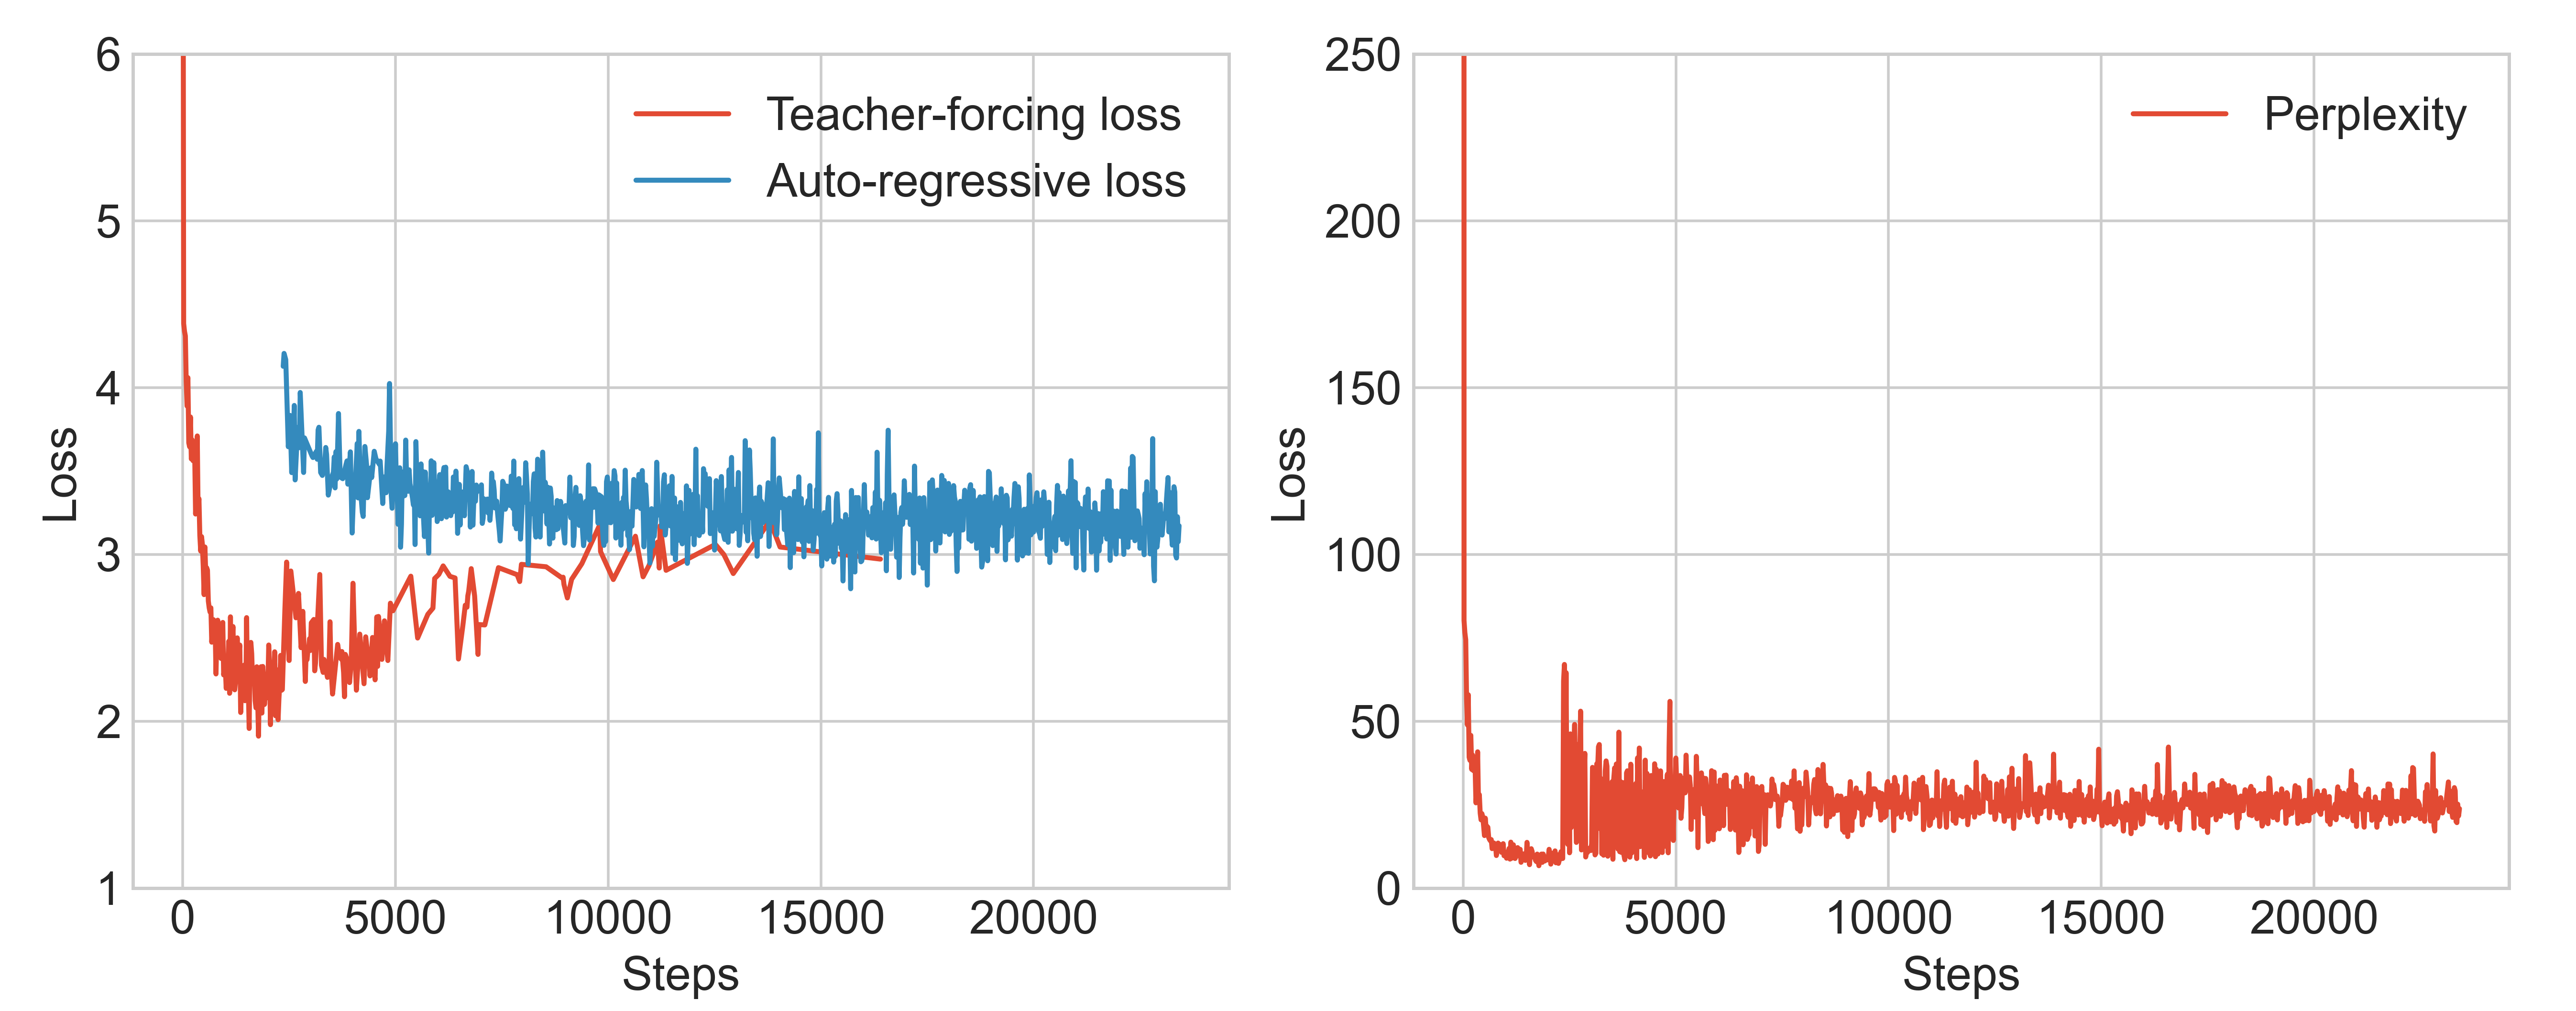
\includegraphics[width=\linewidth]{images/coco_pretraining_losses_ppls.png}
	\caption{Left: Training losses during pretraining the speaker on MS COCO; the colors indicate the pretraining mode, i.e., whether the ground truth caption (teacher-forcing loss, red) or the self-generated token (auto-regressive loss, blue) from the previous timestep was supplied at each timestep. Right: Training perplexity during pretraining of the speaker on MS COCO.}
	\label{fig:coco_pretraining}
\end{figure}  

\begin{figure}
	\centering
	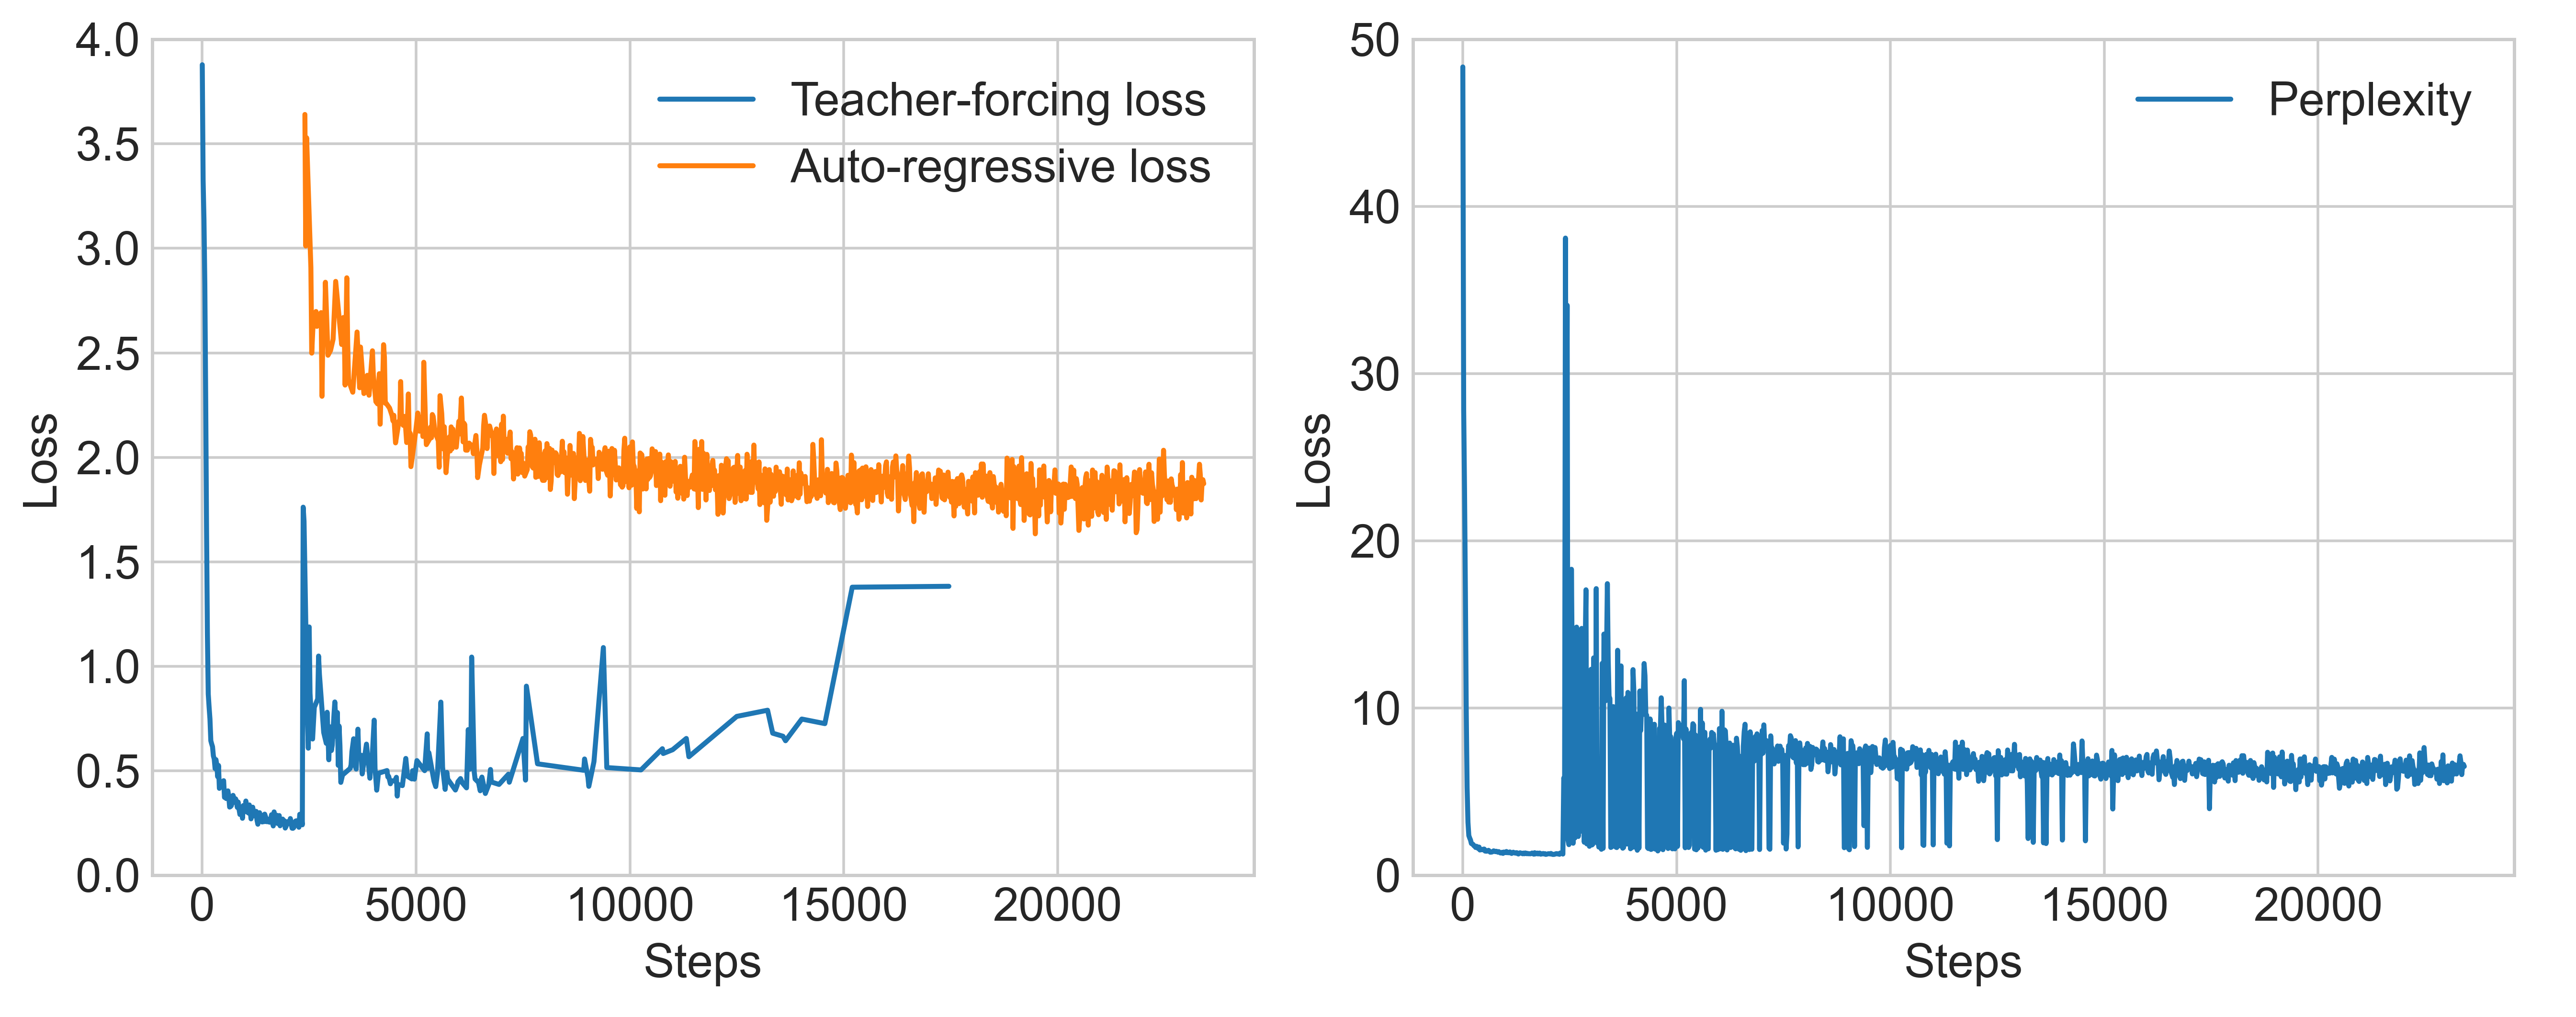
\includegraphics[width=\linewidth]{images/3dshapes_pretraining_losses_ppls.png}
	\caption{Left: Training losses during pretraining the speaker on the exhaustive 3Dshapes dataset; the colors indicate the pretraining mode, i.e., whether the ground truth caption (teacher-forcing loss, blue) or the self-generated token (auto-regressive loss, orange) from the previous timestep was supplied at each timestep. Right: Training perplexity during pretraining of the speaker on 3Dshapes.}
	\label{fig:3dshapes_pretraining}
\end{figure}  

\begin{figure}
	\centering
	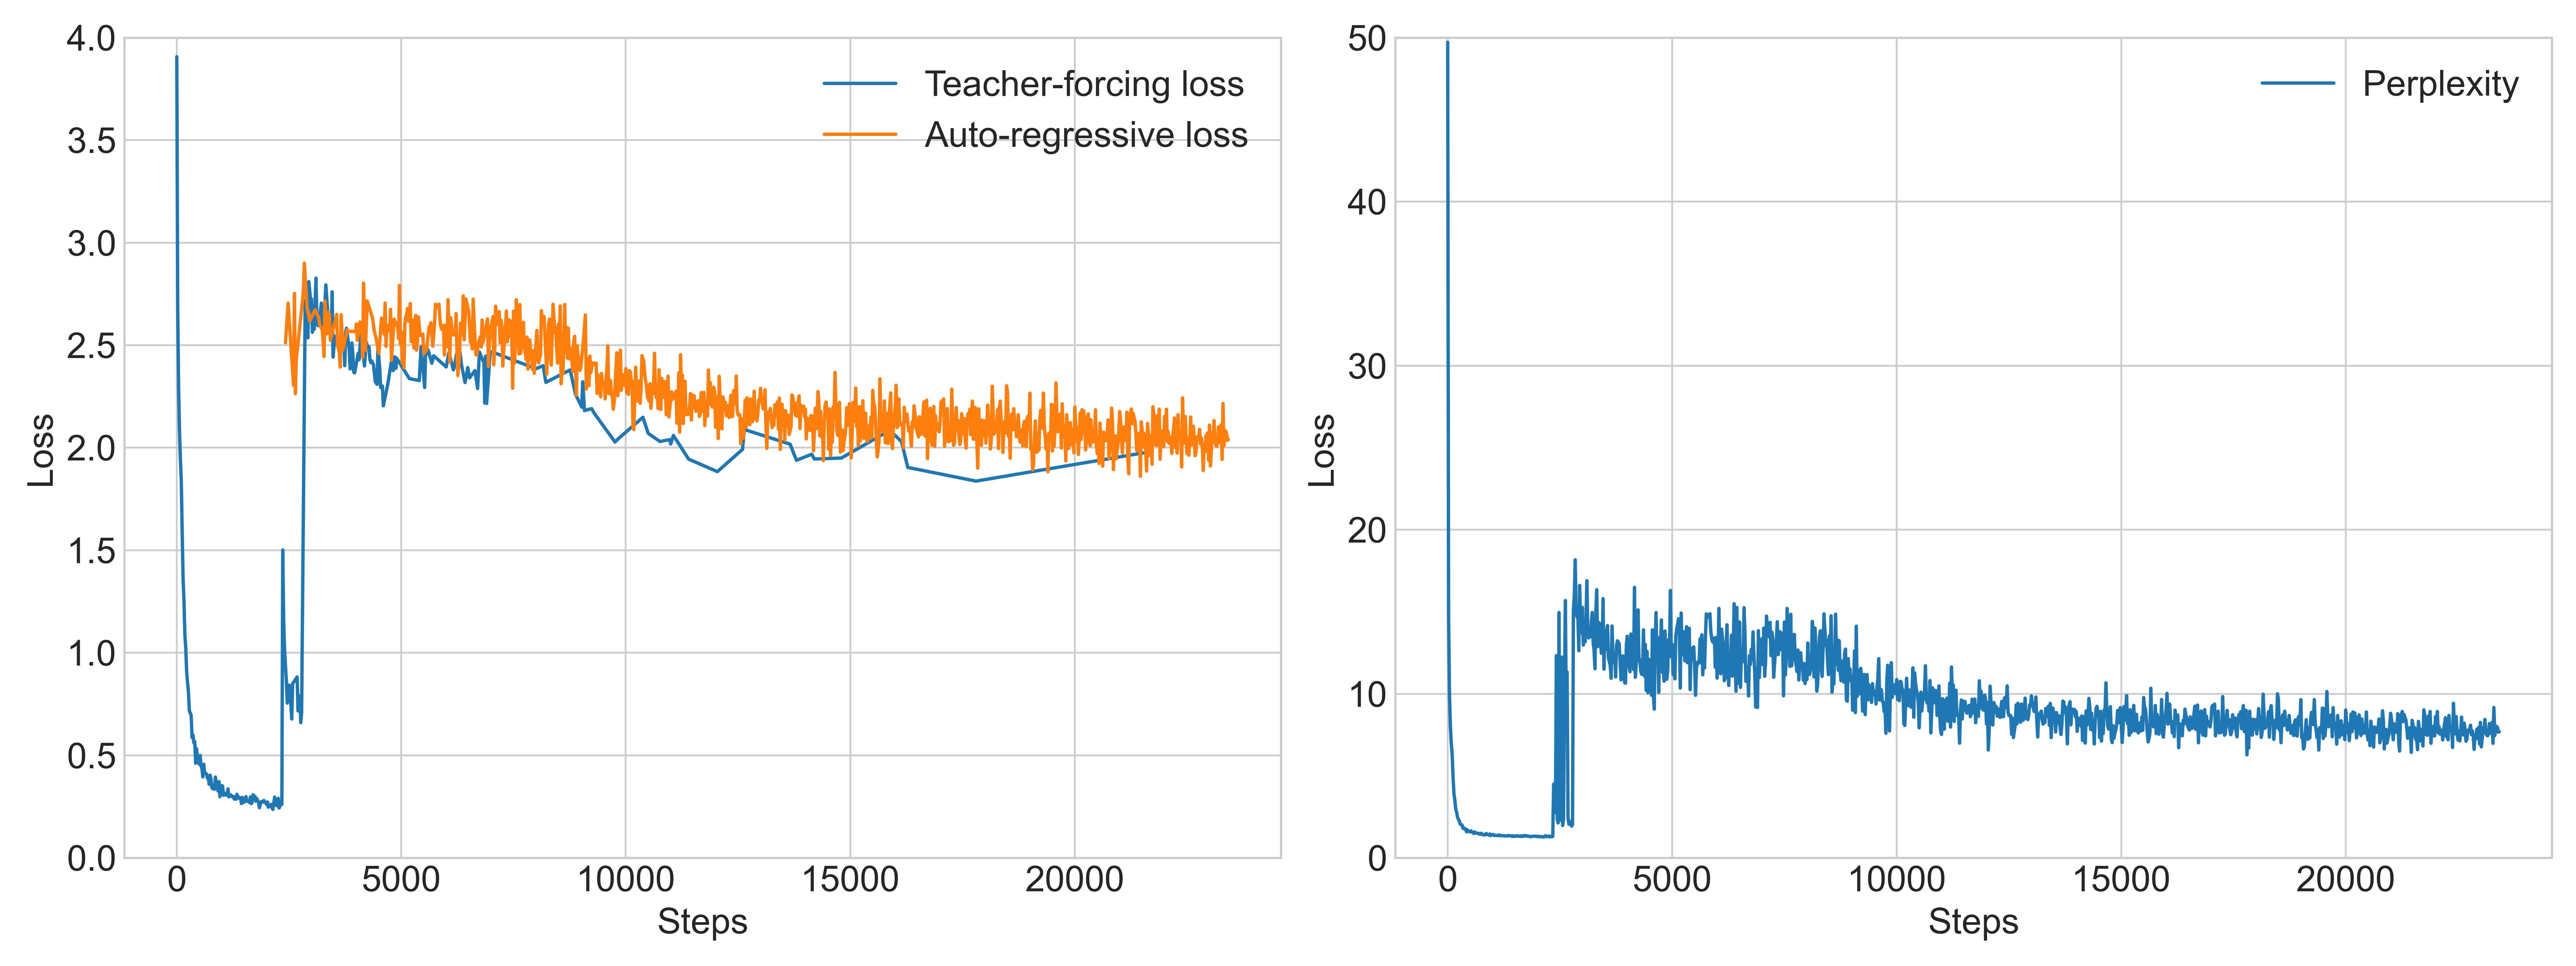
\includegraphics[width=\linewidth]{images/3dshapes_wShort_pretraining_losses_ppls.png}
	\caption{Left: Training losses during pretraining the speaker on the 3Dshapes dataset which includes both short and exhaustive captions; the colors indicate the pretraining mode, i.e., whether the ground truth caption (teacher-forcing loss, blue) or the self-generated token (auto-regressive loss, orange) from the previous timestep was supplied at each timestep. Right: Training perplexity during pretraining of the speaker on 3Dshapes.}
	\label{fig:3dshapes_pretraining_wShort}
\end{figure}  
%Table with image caption quality metrics of the pretrained speakers. Add same metrics of the speaker agents after ref games as rows to the same table. 

\begin{table}[]
	\begin{tabularx}{\textwidth}{|X|l|l|l|l|l|l|l|}
		\hline
		\textbf{Model name}                                    & \textbf{B-1} & \textbf{B-2} & \textbf{B-3} & \textbf{B-4} & \textbf{M} & \textbf{C} & \textbf{Val. loss} \\ \hline
		Pretrained MS speaker                             & 0.408           & 0.137           & 0.042           & 0.013           & 0.116           & 0.165          & 4.079                    \\ \hline
		MS Baseline, random, $\lambda_s = 0$      &   0.405              &      0.130           &     0.036            &     0.009            &     0.116            &     0.177           &           4.124               \\ \hline
		MS Baseline, random, $\lambda_s = 0.25$   &          0.413       &       0.134          &      0.041          &       0.015          &       0.116          &       0.189        &           4.074               \\ \hline
		MS Baseline, random, $\lambda_s = 0.5$   &          0.397       &       0.124          &      0.036          &       0.012          &       0.115          &       0.170         &           4.082               \\ \hline
		MS Baseline, random, $\lambda_s = 0.75$   & 0.407           & 0.133           & 0.037           & 0.010           & 0.116           & 0.178          & 4.056                    \\ \hline
		MS Baseline, random, $\lambda_s = 1$   &    0.405             &   0.125              &    0.033             &  0.000              &         0.115        &       0.181         &         4.066                 \\ \hline
		MS Baseline, similar, $\lambda_s = 0.75$  &                 &                 &                 &                 &                 &                &                          \\ \hline
		MS fixed listener, random, $\lambda_s = 0.75$  &        0.393         &       0.132          &        0.040         &      0.011           &      0.113           &        0.177        &       4.117                   \\ \hline
		Pretrained 3D speaker                            & 0.671           & 0.343           & 0.163           & 0.077           & 0.283           & 1.026          & 2.091                    \\ \hline
		3D Baseline, random, $\lambda_s = 0$     &                 &                 &                 &                 &                 &                &                          \\ \hline
		3D Baseline, random, $\lambda_s = 0.25$   &                 &                 &                 &                 &                 &                &          2.082                \\ \hline
		3D Baseline, random, $\lambda_s = 0.5$   &                 &                 &                 &                 &                 &                &         2.179                 \\ \hline
		3D Baseline, random, $\lambda_s = 0.75$  & 0.672           & 0.340           & 0.159           & 0.074           & 0.284           & 1.068          & 2.089                    \\ \hline
		3D Baseline, random, $\lambda_s = 1$   &                 &                 &                 &                 &                 &                &                          \\ \hline
		3D Baseline, similar, $\lambda_s = 0.75$ & 0.673           & 0.335           & 0.152           & 0.070           & 0.279           & 1.033          & 2.103                    \\ \hline
		\pt{FILL ME with more expts} &                 &                 &                 &                 &                 &                &                          \\ \hline
	\end{tabularx}
\caption{\label{tab:eval_metrics_refgame} Caption evaluation metrics and the validation loss on a heldout dataset, computed for the initial pretrained speakers and the speakers after training on the reference game. \textbf{B} denotes BLEU, \textbf{M} the METEOR score, \textbf{C} the CIDEr score, MS the MS COCO dataset and 3D the 3DShapes dataset. ``Baseline'' refers to the setup wherein the listener is trained jointly with the speaker, using pure decoding. ``Random'' refers to speakers trained on random target-distractor pairs; ``similar'' refers to speakers trained on similar target-distractor pairs.}
\end{table}

The speaker agents were pretrained for both the MS COCO and 3Dshapes experiments. Conceptually, the model was pretrained in order to learn the statistical properties of English, i.e., ``learn to speak'', before being finetuned on the functional reference game task. This is can be motivated as providing general \textit{task-uncoditional} linguistic capabilities to the speaker which she can the transfer to specific tasks.

Both speakers were pretrained in a supervised fashion by sampling tuples of the form $(i_t, i_d, c_t)$ where $i_t, i_d$ are the target and distractor images, and $c_t$ in the target ground truth caption. The models were pretrained on 30,000 images selected at random from the respective dataset; for each image, the model saw five available ground truth captions. 
The pretraining was accomplished with the cross-entropy loss. Both models were trained for ten epochs.

As described in Section \ref{model_pretraining}, there are different strategies for pretraining the speaker. Based on initial exploratory experiments reported in Appendix \ref{app:grid_search}, all speakers were pretrained using an exponentially decreasing teacher-forcing rate $0.5^{epoch-1}$, transitioning to auto-regressive training with pure decoding. That is, in the auto-regressive mode the model was fed its own predicted token from the previous timestep during training; that token was generated by pure sampling. Speakers for both datasets were pretrained in this set up. Figure \ref{fig:coco_pretraining} shows the pretraining dynamics of the MS COCO speaker, Figure \ref{fig:3dshapes_pretraining} shows the dynamics of the 3Dshapes speaker pretrained on exhaustive captions. Additionally, another 3Dshapes speaker was pretrained on both exhaustive and short captions from the second 3Dshapes annotations dataset. More precisely, for each image, five ground truth captions were selected, sampling at random whether three out of five captions were short or exhaustive. This additional speaker was trained for the experiments with short captions (addressing \textbf{H10}) in order to induce a bias towards actually generating short captions from pretraining; otherwise, without explicit pressure towards generating shorter messages, the speaker would be expected to produce exhaustive caption length messages \parencite[cf., e.~g.,][]{hupkes2020compositionality}. The pretraining results can be seen in Figure \ref{fig:3dshapes_pretraining_wShort}.

The evaluation of their image captioning capabilities on standard metrics (introduced in Chapter \ref{chapter02}) after pretraining can be found in Table \ref{tab:eval_metrics_refgame}. The metrics were computed in a held out validation split with 5000 unique images and respective captions. Comparing the pretrained speakers to state-of-the-art image captioning model peformance in Table \ref{tab_coco_metrics_ref}, it is apparant that the speakers perform somewhat worse iin terms of standard caption evaluation metrics. It is hypothesized that this is due to the mixed teacher-forcing and auto-regression training mode. It is conjectured that the speaker quality only might affect the absolute performance and drift metric values, but the qualitative comparisons between experiments will remain unaffected because all experiments are based on the same pretrained speakers.

Furthermore, all language drift metrics are computed for the pretrained models which arguably present a baseline for linguistic capabilities, before any deterioration might take place due to task optimization (see Tables \ref{tab:coco_drift_metrics_basic}, \ref{tab:3dshapes_drift_metrics_basic}).

\subsection{MS COCO: Baseline Experiments}
\label{expt:coco_baseline}

\begin{table}[]
	\begin{tabularx}{\textwidth}{|X|l|l|X|X|X|X|}
		\hline
		\textbf{Model name}                                    & \textbf{log $P(m)$} & \textbf{log $P(m \mid i)$} & \textbf{Overlap (d)} & \textbf{Overlap (c)} & \textbf{Listener acc (random)} & \textbf{Listener acc (similar)} \\ \hline
		Ground truth validation captions               &     -108.566            &          -80.399             &    9.147           &       0.038          &            &                           \\ \hline
		Pretrained MS speaker               &      -131.598            &           -62.385             &          1.194            &           0.003           & 0.912 (random listeners)                 &                                           \\ \hline
		MS Baseline, random, $\lambda_s = 0$      &     -131.890              &         -63.319               &        1.259       &         0.003             &             0.924                             &                                           \\ \hline
		MS Baseline, random, $\lambda_s = 0.25$    &      -133.954             &          -65.533              &          1.173            &       0.004               &           0.935                               &                                           \\ \hline
		MS Baseline, random, $\lambda_s = 0.5$      &         -133.595         &           -67.904             &        1.106              &        0.001              &             0.890                             &                                           \\ \hline
		MS Baseline, random, $\lambda_s = 0.75$   &       -135.910            &             -71.819          &        1.197              &        0.000              & 0.953                                    &                                           \\ \hline
		MS Baseline, random, $\lambda_s =1$  &      -136.762             &          -70.454              &         1.125             &          0.001            &                   0.914                       &                                           \\ \hline
		MS Baseline, similar, $\lambda_s = 0.75$  &                   &                        &                      &                      &                                          &                                           \\ \hline
		MS, random, fixed listener, $\lambda_s = 0$  &         -130.624         &           -62.095             &     1.201                 &        0.003              &                          0.888                &                                           \\ \hline
		MS, random, fixed listener, $\lambda_s = 0.75$  &         -134.408          &           -67.627             &     1.042                 &        0.003              &                          0.881                &                                           \\ \hline
	\end{tabularx}
\caption{\label{tab:coco_drift_metrics_basic} Language drift metrics and listener test accuracies on different pairs. 
	``Baseline'' refers to the setup wherein the listener is trained jointly with the speaker, using pure decoding. MS refers to the MS COCO dataset. ``Random'' refers to speakers trained on random target-distractor pairs; ``similar'' refers to speakers trained on similar target-distractor pairs. ``Overlap (d)'' refers to the discrete overlap metric, ``overlap (c)'' to continuous overlap.}
\end{table}

The baseline experiment on MS COCO was conducted on 30,000 images which were not used during pretraining. The target-distractor pairs were constructed at random, and each target appeared in five pairs such that the structural loss could be minimized with respect to all five available ground truth captions. Pure decoding was used for decoding the speaker's message, and the weight of the structural loss was $\lambda_s = 0.75$. The weight of the functional loss was $\lambda_f = 0.25$, respecitvely. These configurations are treated as the baseline experiment since preliminary explorations revealed that these are the minimal requirements for a successful reference game (see Appendix \ref{app:grid_search} for details). The training dynamics can be seen in Figure \ref{fig:coco_baseline_075_speaker_loss_listener_acc}.

\begin{figure}
	\centering
	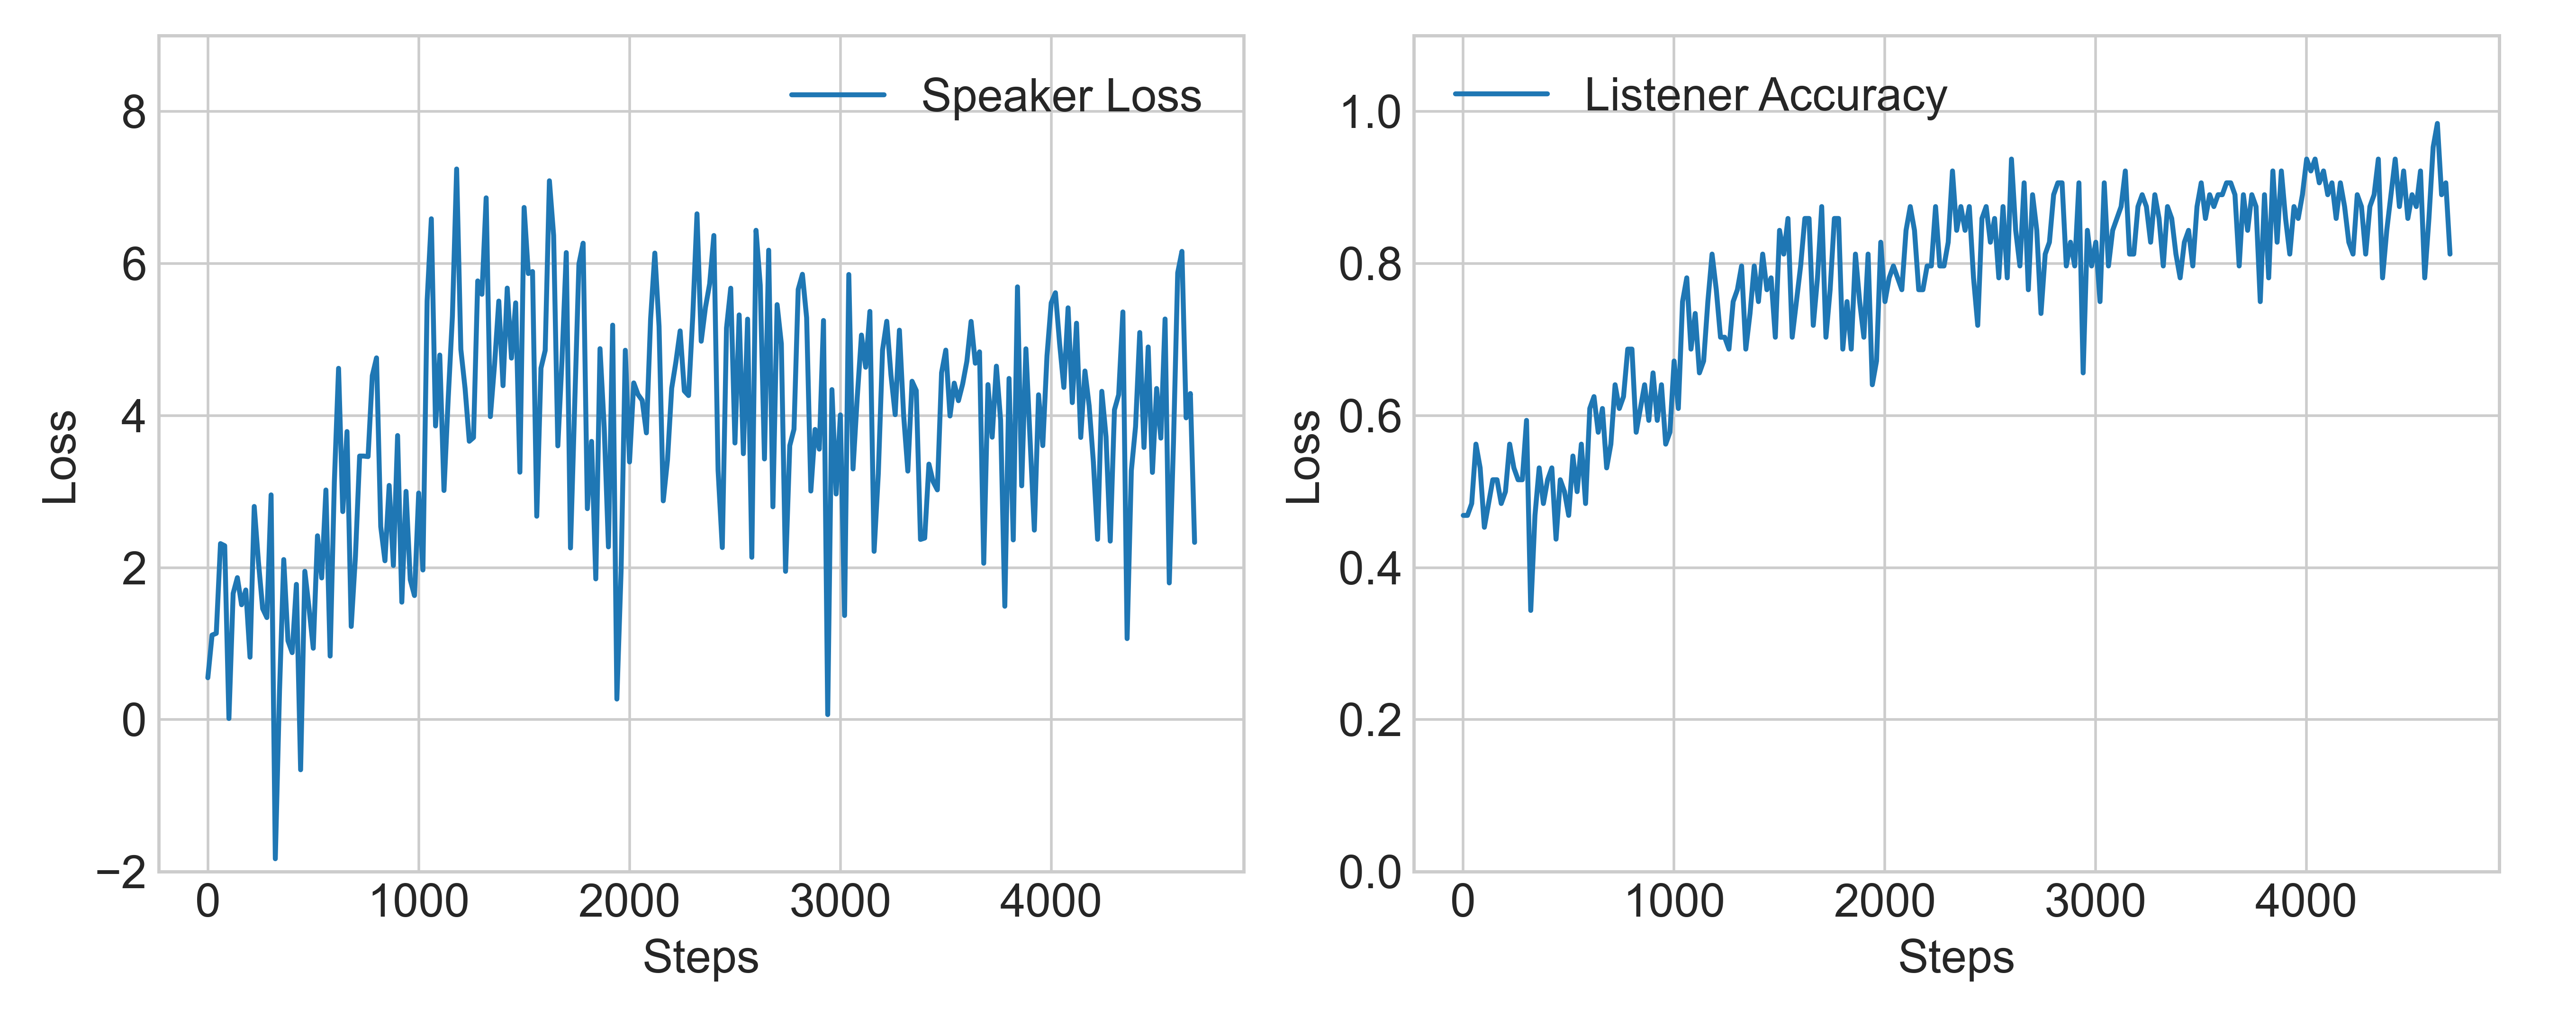
\includegraphics[width=\linewidth]{images/coco_refgame_4000_pure_075_random.png}
	\caption{Training results of the baseline MS COCO experiment (pure decoding, $\lambda_s = 0.75$). Left: Total speaker train loss. Right: Listener train accuracy.}
	\label{fig:coco_baseline_075_speaker_loss_listener_acc}
\end{figure}


\begin{figure}
	\centering
	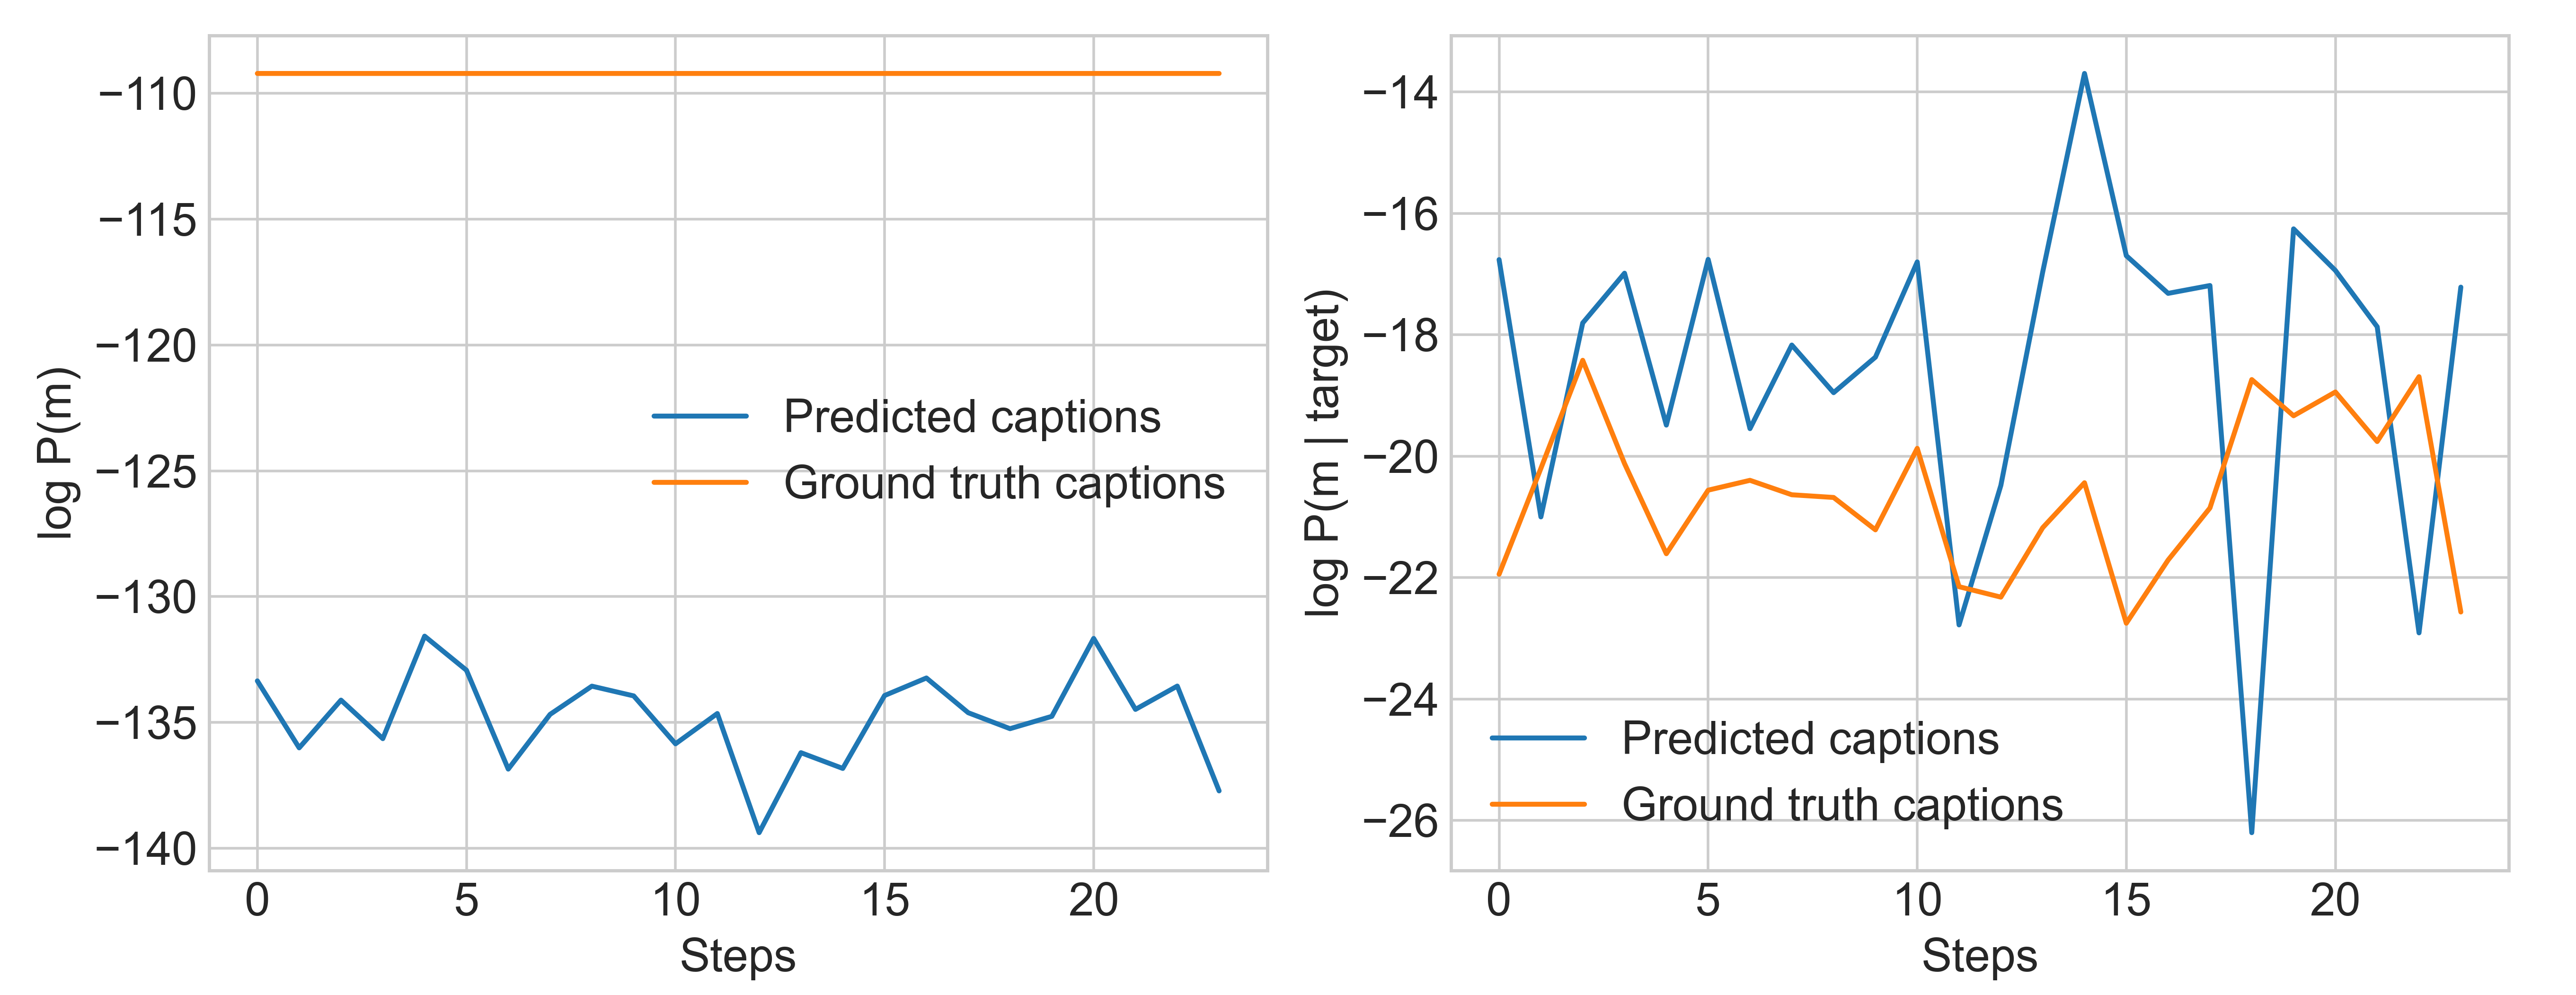
\includegraphics[width=\linewidth]{images/coco_structural_semantic_drift_4000_pure_075_random.png}
	\caption{Drift dynamics computed during training in the baseline MS COCO experiment (pure decoding, $\lambda_s = 0.75$). Higher values indicate less drift. Left: Structural drift of ground truth and predicted captions under the pretrained Transformer XL model. Right: Semantic drift of ground truth and predicted captions under the pretrained speaker model.\protect\footnotemark}
	\label{fig:coco_baseline_075_str_drift}
\end{figure}
\footnotetext{Due to a coding error, semantic drifts were computed using greedy decoding on one image-caption pair only and, therefore, the values vary quite strongly.} 

For computing the test task accuracy, listener accuracy was computed on a held out validation set of 1000 pairs of images which were neither part of pretraining nor the reference game training. The test accuracy of 0.953 in Table \ref{tab:coco_drift_metrics_basic} shows that the agents successfully learned to play the reference game. Furthermore, supporting \textbf{H1} and \textbf{H2}, the language underwent slight deterioration, both syntactically and semantically, compared to the pretrained speaker. More specifically, the average log probability of the generated captions under the pretrained Transformer XL model decreased by 4.312, compated to the log probability of captions generated by the pretrained speaker. Similarly, the conditional log probability of the generated captions given the target images decreased by 9.434, compared to the conditional probability of the captions from the pretrained speaker (Table \ref{tab:coco_drift_metrics_basic}, first two columns, ``Pretrained MS speaker'' vs. ``MS Baseline, random, $\lambda_s=0.75$''). The dynamics of structural and semantic drifts during training can be seen in Figure \ref{fig:coco_baseline_075_str_drift}. To this end, the structural and semantic drift metrics were computed every 200 training steps on 192 held out image pairs. Due to the small size of the decrease as well as the small number of validation batches, no trend can be observed visually.\footnote{The number of metric computation steps was restricted to only three batches due to computational constraints.} 
As for the other drift metrics presented in Table \ref{tab:coco_drift_metrics_basic} (third and fourth columns), only anecdotal differences to the pretrained speaker can be observed: a slight increase in the discrete overlap metric might suggest that the speaker learned to produce messages that are more appropriate for the target compared to the distractor, and, therefore, might be more discriminative. On the other hand, the similarity of embeddings of the ground truth caption and the message decreased relative to the distractor similarity, compared to the pretrained speaker. This might be due to the difficulty to propagate the learning signal all the way to the embedding layer. Furthermore, the comparison to the overlap values of the ground truth captions indicates that the difference in terms of used tookens between target and distractor captions is much more pronounced in the dataset than what is propagated by the trained model (Tab.~\ref{tab:coco_drift_metrics_basic}, first line, third and fourth columns). \pt{check if the following shouldn't go into the discussion section isntead.} However, this is not necessarily indicative of bad discriminative performance. More specifically, the low overlap value might be due to the fact that the generated captions contain words which were not part of the ground truth caption because, for instance, they refer to features which were not mentioned in the descriptive ground truth captions, but were chosen under discriminative pressure by the trained speaker.\footnote{Thanks to Malte Heyen for the discussion which led to this point.} 
Therefore, to sum up, \textbf{H3} is not borne out in this experiment.

\pt{Linear regressions will be computed on the drift values collected during the training.}

Additionally, the fine-tuned speaker was also evaluated with standard image captioning metrics. Table \ref{tab:eval_metrics_refgame} shows that caption quality marginally decreased with respect to almost all metrics, confirming the trend shown by the structural and semantic language drift metrics.

\subsubsection{Varying the structural loss weight}
In order to investigate \textbf{H4}, this experiment on MS COCO is also conducted with different structural loss weights $\lambda_s \in \{0, 0.25, 0.5, 1\}$. The training results (i.e., the speaker losses and listener accuracies during training) can be seen in Figure \ref{fig:coco_baseline_speaker_loss_listener_acc_all}. The main observation that can be made regarding the training dynamics is that the magnitude of the loss strongly depends on the weight of the structural loss $\lambda_s$---the smaller the weight, the larger are the total loss values (Fig.~\ref{fig:coco_baseline_speaker_loss_listener_acc_all}, left). This can be attributed to the larger weight of the functional loss, respectively, which is computed with REINFORCE and might be subject to stronger variance \parencite[cf.][]{havrylov2017emergence}. However, varying the weight does not have visible effects on the listener's ability to learn the reference game (Fig.~\ref{fig:coco_baseline_speaker_loss_listener_acc_all}, right). 
This is supported by the similar test listener accuracy values in Table \ref{tab:coco_drift_metrics_basic} (fifth column). If anything, against general intuitions from the literature, the task performance is slightly worse with higher functional pressure (test accuracy of 0.924 with functional loss only), compared to higher structural pressure (test accuracy of 0.953 with $\lambda_s = 0.75$). But consistent with intuition, the accuracy in the experiment where the speaker was trained with structural pressure only ($\lambda_s = 1$), the listener accuracy is almost identical to the listener accuracy computed against the pretrained speaker. This confirms that training the speaker with the structural loss only amounts to further training the pretrained model, which was already pretrained to convergence (see Fig.~\ref{fig:coco_pretraining}) and, therefore, does not improve much.

%This could indicate that the listener is flexible enough to adapt to the speaker's messages, essentially independently of their nature. This hints at speaker-listener co-adaptation. 
\begin{figure}
	\centering
	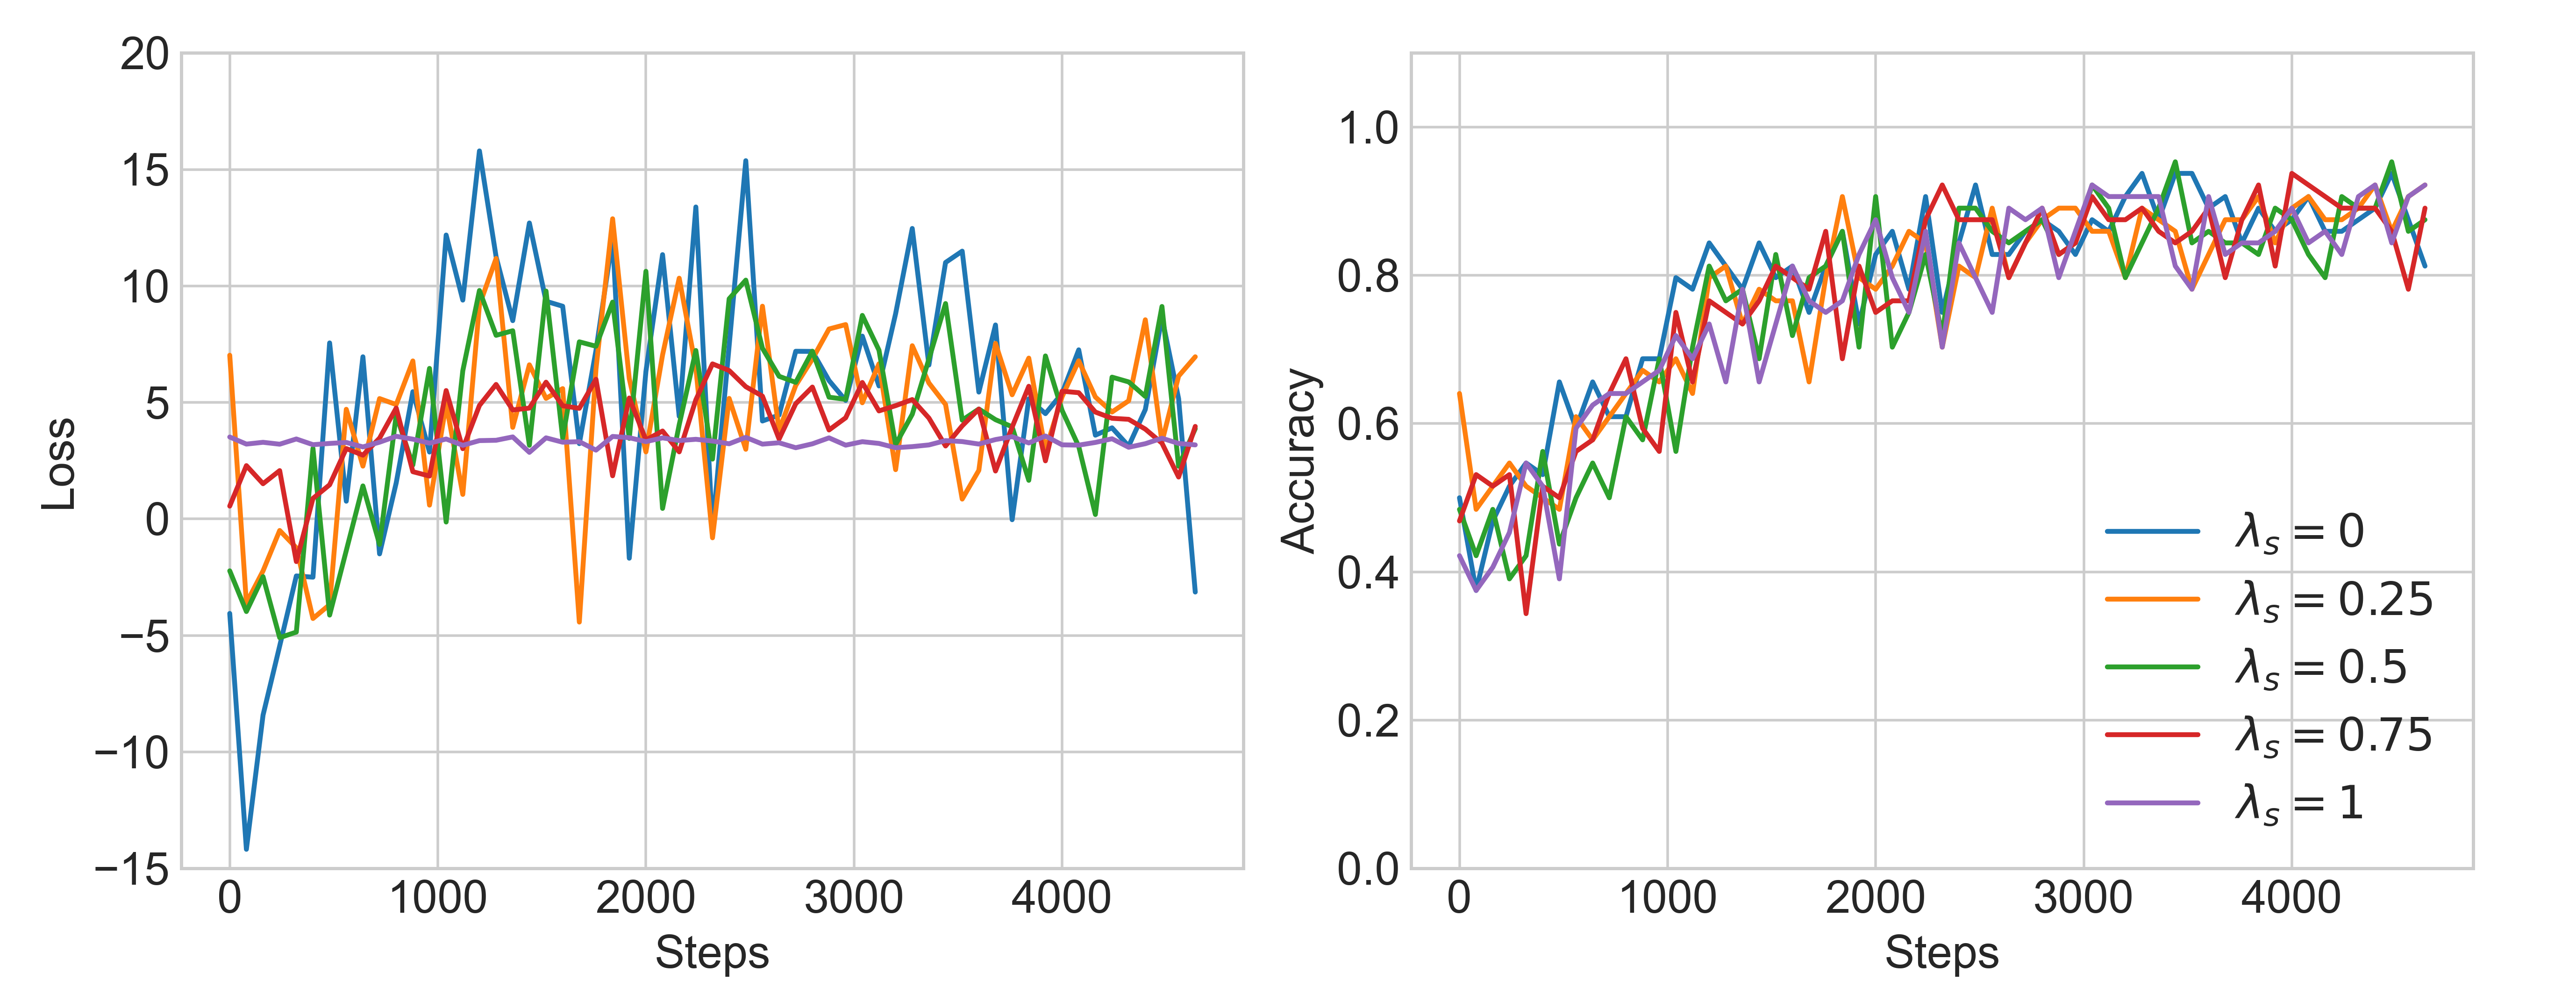
\includegraphics[width=\linewidth]{images/coco_refgame_4000_pure_all_Ls_random.png}
	\caption{Training results of the MS COCO experiment with varying $\lambda_s$ (pure decoding). Left: Total speaker train loss. Right: Listener train accuracy.}
	\label{fig:coco_baseline_speaker_loss_listener_acc_all}
\end{figure}

Table \ref{tab:coco_drift_metrics_basic} also provides a comparison of the drift metrics for the different loss configurations. Based on naive comparison, if anything, the structural and semantic drifts are smaller when the structural pressure on the speaker is \emph{smaller}, contrary to a priori intuition. That is, when the pressure to stay close to the initially learned image captioning language distribution is smaller, the produced messages have a higher likelihood both under the pretrained LM and the pretrained speaker. The absense of a clear difference between the drift results is also supported by the drift dynamics computed during training (see Fig. \ref{fig:coco_baseline_str_sem_drift_all}). 
The drift values for the experiment with $\lambda_s = 0$ also speak against \textbf{H1} and \textbf{H2}. Somewhat surprisingly, semantic drift values are lower for the generated captions compared to the ground truth captions (Fig.~\ref{fig:coco_baseline_str_sem_drift_all}), indicating that the generated captions are generally more likely given the target image, than the ground truth captions, under the pretrained speaker model. This could be attributed to the auto-regressive pretraining of the speaker, which might have resulted in generally better performance in the auto-regressive generation mode, compared to teacher-forcing based ground truth availability \pt{cite intro chapter}.

One reason this might be due to is that the drift computation employs greedy decoding, as is common practice for inference time performance. However, during reference game training, the speaker uses pure decoding. This difference in decoding modes might be responsible for the seemingly unexpected trend. As to the structural drift, it seems that the model trained with \emph{less} structural pressure produces messages that are more likely under a pretrained language model. However, it should be noted that the pretrained speaker produces messages that are not very well-formed on a surface level \pt{as can be seen from these examples, ADD}, most likely due to the involvement of the auto-regressive pretraining mode (\pt{see pretraining section---add details and examples there.}). Therefore, it might be expected that a speaker which is more strongly forced to stay close to the pretraining language distribution produces less structurally well-formed sentences, under a pretrained LM. The more functionally oriented speaker, on the other hand, might by chance produce better sentences, even if the respective learning signal is not related to the LM. Lastly, it could be hypothesized that these drift results are rather snapshots of the speaker's performance, especially for the speakers with lower $\lambda_s$, since their policies did not converge after training the agents for only two training epochs, as can be seen from the respective loss plot (Fig. \ref{fig:coco_baseline_speaker_loss_listener_acc_all}, left). 
Turning towards the other drift metrics in Table \ref{tab:coco_drift_metrics_basic}, again, there is no indication of a clear trend in connection to the strucutral loss weight. Nevertheless, the discrete overlap has the highest value for the $\lambda_s = 0$ experiment (0.065 higher than for the pretrained speaker), indicating that the strong functional pressure on the speaker might have led to generating captions capturing more of the target image's properties.

This seeming insensitivity of the overlap metrics might be due to several reasons. First, due to a lack of comparability to other work, further experiments, e. g., replicating existing work, involving these mterics need to be conducted in order to properly assess their plausibility. \pt{this might be material for discussion}. Second, the continuous overlap might be subject to vanishing gradients which become too small over the backpropagation steps through time of the message sequence in order to affect the embedding layer \parencite[cf.][]{jaeger2002tutorial}. Finally, it might be the case that generally the training just did not proceed for a sufficient number of epochs for the functional loss to take effect, as literature has argued that REINFORCE based training, especially given large action spaces like the one at hand, is slower to converge \parencite{havrylov2017emergence} \pt{look into Havrylov again: is convergence always in terms of listener performance, or speaker loss too?}.

The speakers trained with the different loss configurations were also evaluated using image captioning metrics; the results are reported in Table \ref{tab:eval_metrics_refgame}. Generally, they also follow the trends indicated by the drift metrics, although the differences in values are marginal.

To sum up, given the presented training configurations, \textbf{H4} is not supported by the results. However, based on the grid search over speaker configurations conducted prior to the main experiments (see the difference in reference game performances in Appendix \ref{app:grid_search}, Fig.~\ref{fig:coco_grid_Ls_decoding_TF_only}), one might hypothesize that the presence of effects of the structural loss weight is connected to the presence of auto-regressive pretraining of the speaker agent. That is, it could be critical that the speaker is already pretrained with the caption generation mode, as it then plays a role for the structural loss computation the reference game. Follow-up experiments regarding this effect of pretraining mode would fill a gap in the extant literature \parencite[but see][for related work]{lowe2020interaction}.

\begin{figure}
	\centering
	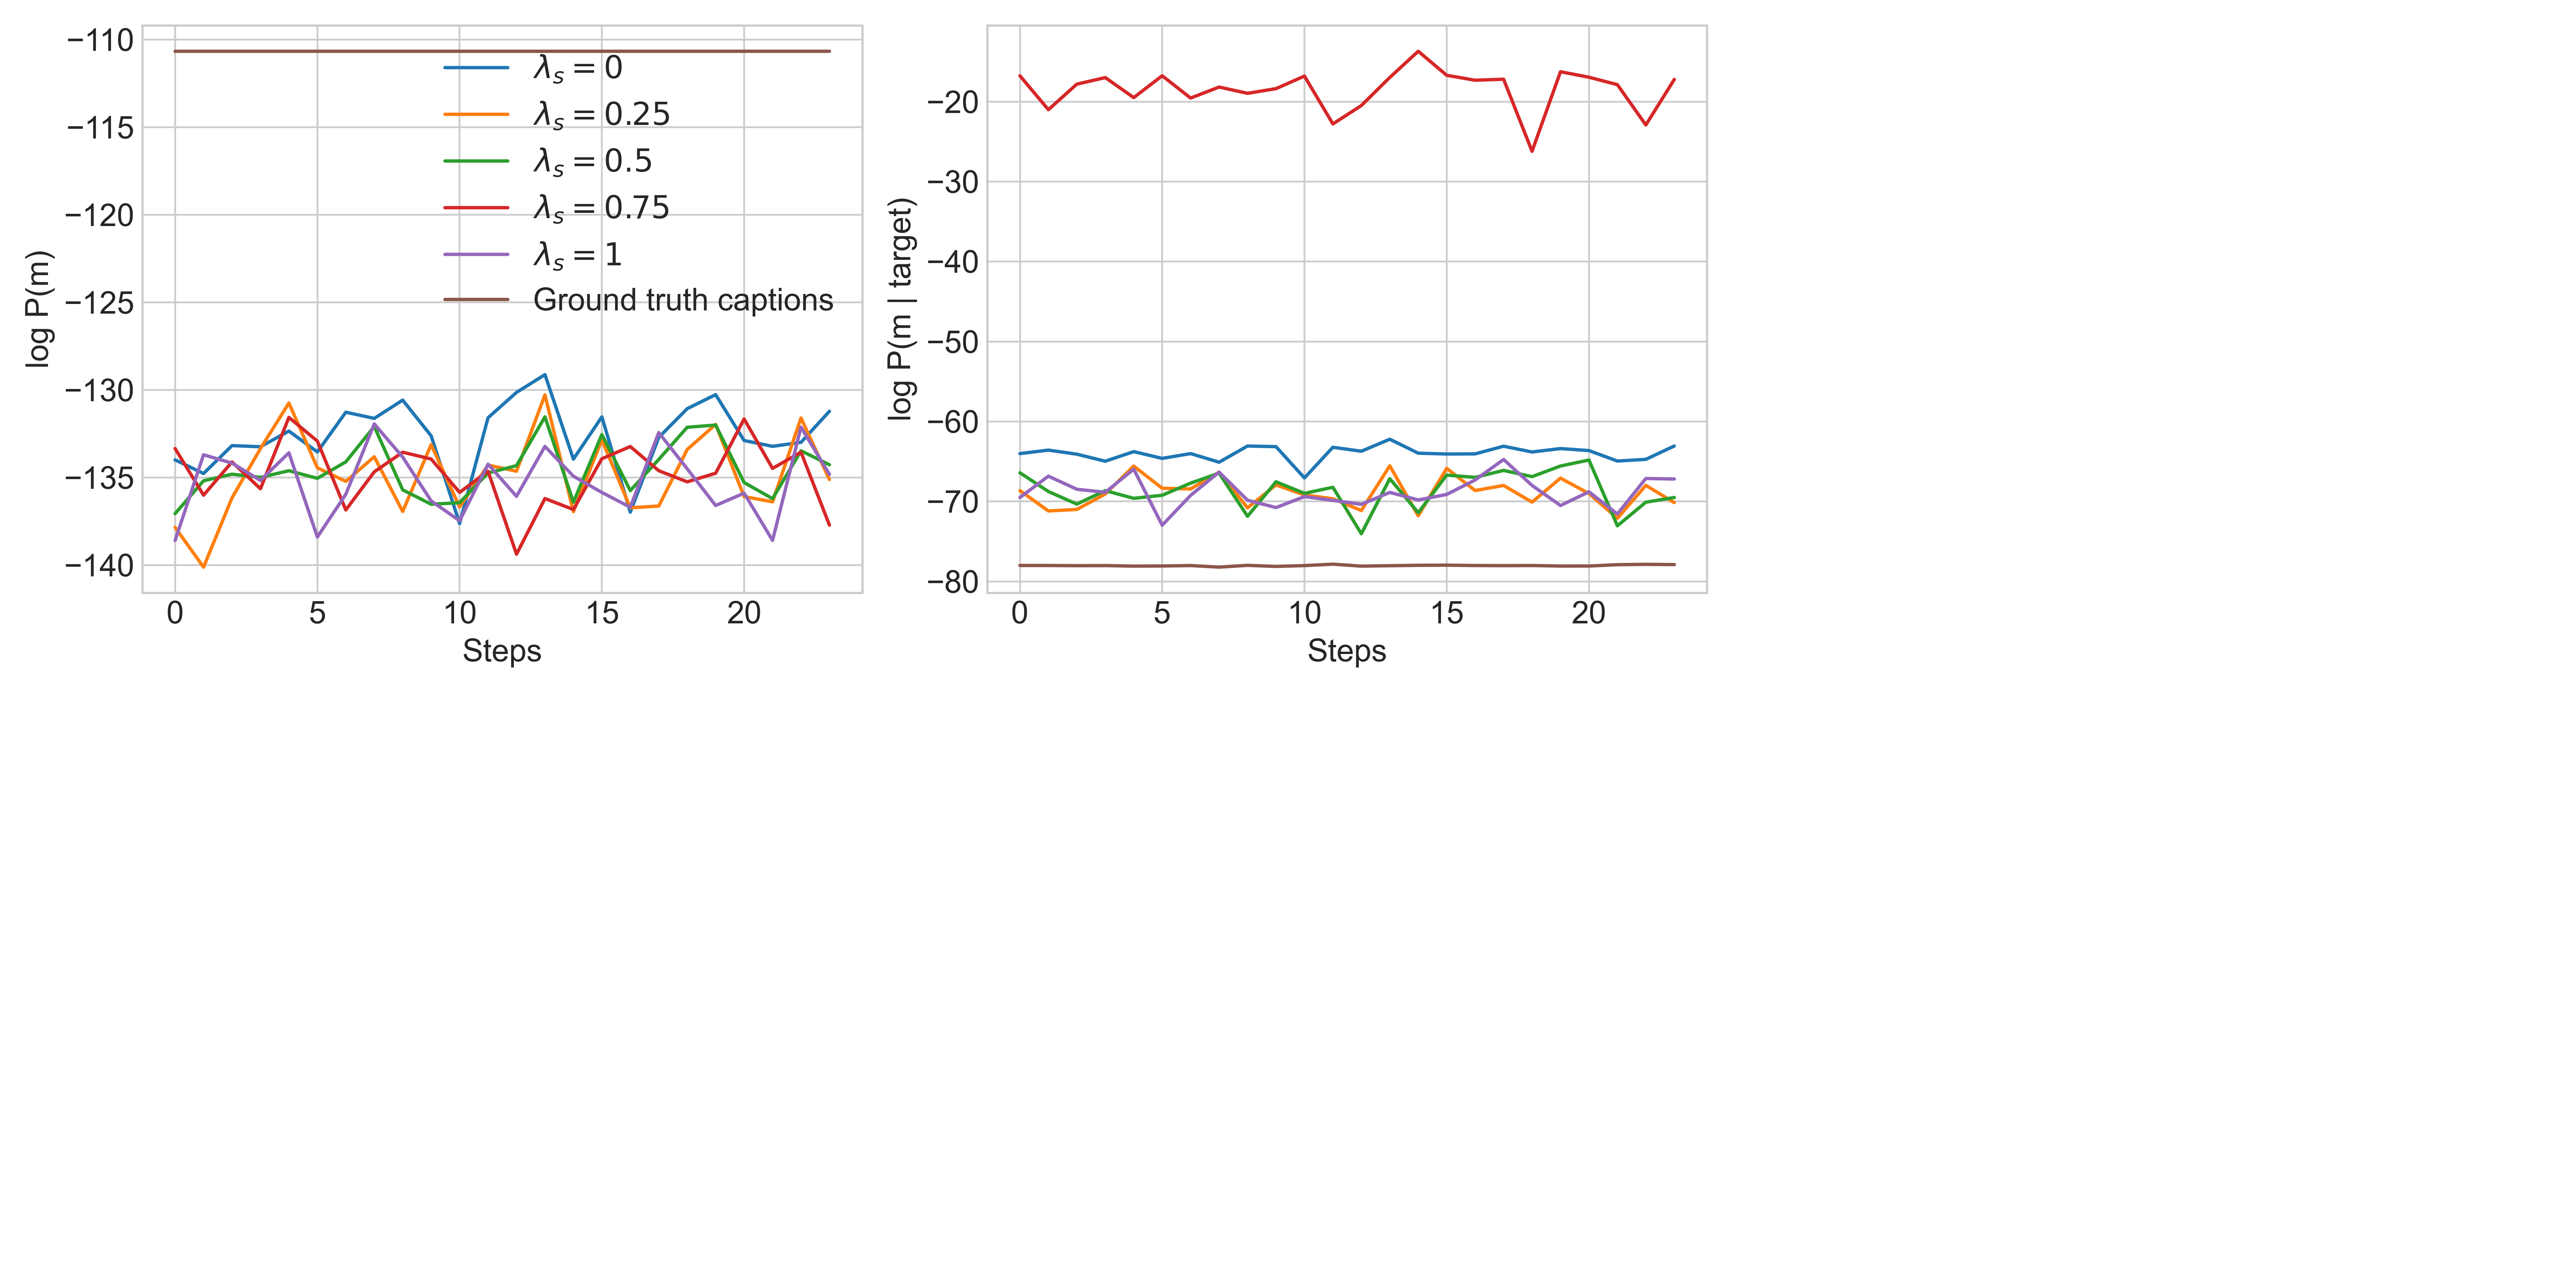
\includegraphics[width=\linewidth]{images/coco_structural_semantic_drift_4000_pure_L_S_all_random.png}
	\caption{Drift dynamics computed during training in the baseline MS COCO experiments (pure decoding) with varying $\lambda_s$ weights. Higher values indicate less drift. Left: Structural drift of ground truth and predicted captions under the pretrained Transformer XL model. Right: Semantic drift of ground truth and predicted captions under the pretrained speaker model. Due to a coding error, the semantic drift of the $\lambda_s = 0.75$ model is as represented the mean validation conditional log probability from Tab.~\ref{tab:coco_drift_metrics_basic}.}
	\label{fig:coco_baseline_str_sem_drift_all}
\end{figure}


\pt{After trying again with the old speaker and the grid search 15 000 images, it is cear that the variation of Ls had an effect on the teacher-forced speaker only, not on the auto-regressive one. Therefore, actually do a rather detailed Appendix and discuss this from a cognitive plausibility perspective in terms of the actual pretraining mode, and also in terms of importance of this hyperparameter of the experiment which is usually not discussed in the literature. But also check grid search files on Omniboard. Padding was also a difference bw final and grid search experiments.}

\subsection{MS COCO: Similar Pairs Experiments}

\textbf{H5}
% For evaluating the random pairs vs the similar pairs, it would be good to conduct tests with similar and random pairs for both agents, and the especially look at discrete overlaps on the similar pairs, and check if the agents learned to distinguish the images more graunlarly. If not, discuss this as an interesting result, wherein it is actually easier for humans if the discriminative feature is clear as opposed to more distinct images (check if it cognitively plausible though). Find a way to check the granularity of produced descriptions / categories (maybe via simple POS tagging / partial parsing somehow).


\subsection{MS COCO: Fixed Listener Experiments}
\label{exp:coco_fixed_listener}
In order to investigate \textbf{H6}, a reference game with pure decoding and $\lambda_s=0.75$ was conducted with a \emph{fixed} listener. That, is the speaker was fine-tuned to produce discriminative captions while being provided the task success signal by an already pretrained listener which was not further trained during the reference game, as opposed to receiving the task success signal from a listener which learns to complete the task and ground the speaker's messages during the reference game. To this end, the listener was pretrained for four epochs to optimally interpret ground truth image captions. The same images as for the speaker pretraining were used. That is, the listener agent saw random pairs of images and received the ground truth caption for the target and was optimized to identify the target. After pretraining, the test accuracy on the ground truth captions of a held out dataset of 1000 images was 0.963. The test accuracy on messages generated by the pretrained speaker for the same images was 0.902.

The goal of this experiment is to investigate language drift in absense of speaker-listener co-adaptation which arises when the two agents are trained together. By having a fixed pretrained listener, intuitively, the speaker cannot improve the message discriminativity by finding `loopholes' and establishing specific conventions with the listener, and should be forced to use the ground truth grounding of the messages.

\begin{figure}
	\centering
	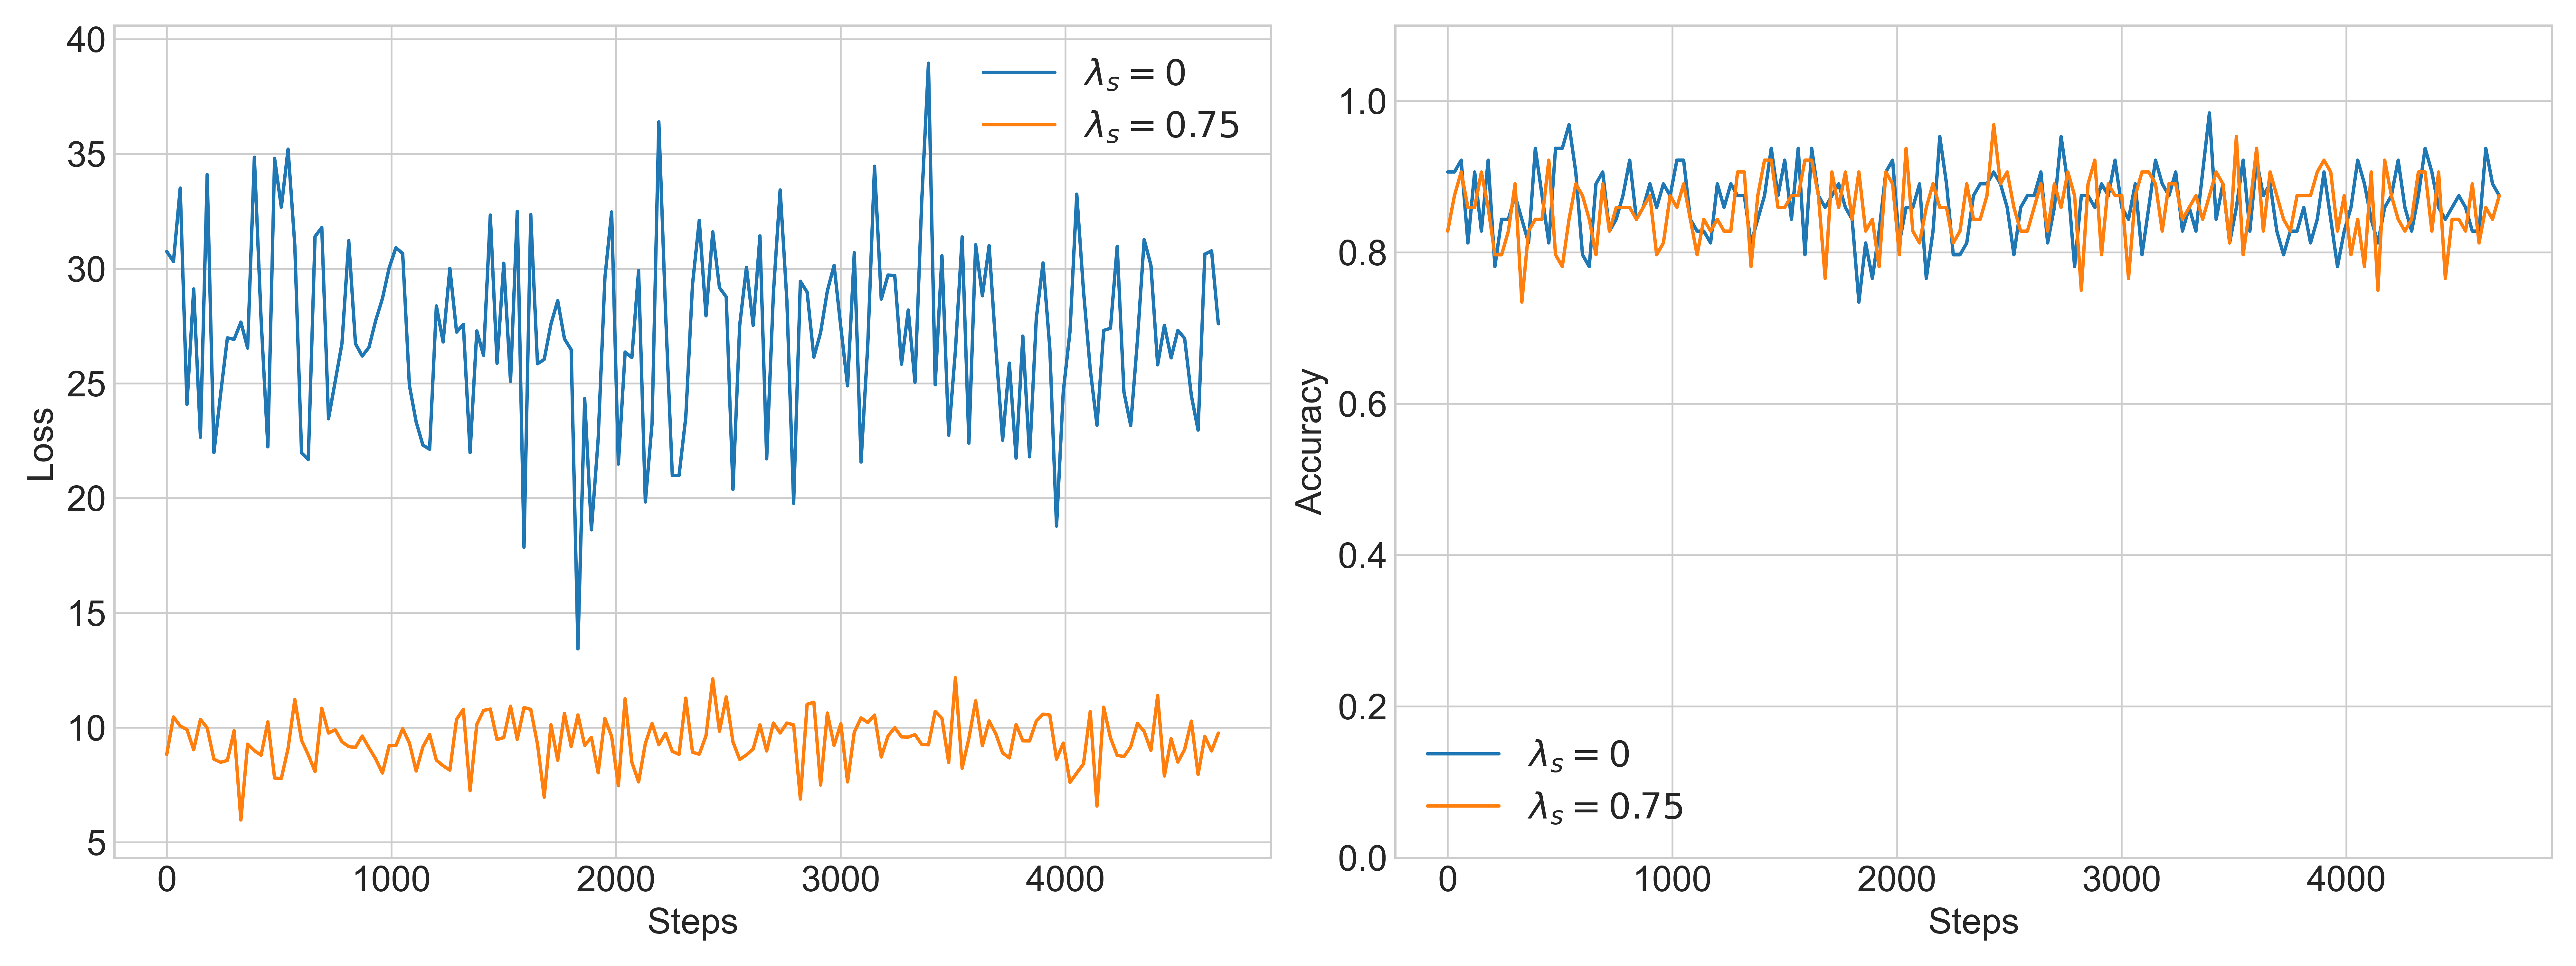
\includegraphics[width=\linewidth]{images/coco_fixedListener_baseline_random_0_075_losses.png}
	\caption{Training results of the MS COCO experiment with a fixed listener (pure decoding, $\lambda_s=0$ vs. $\lambda_s=0.75$). Left: Total speaker training loss. Right: Listener train accuracy.}
	\label{fig:coco_fixed_listener_speaker_loss_listener_acc_075}
\end{figure}

The training and testing prcedures were idetical to previously described random image pairs experiments. The training dynamics can be seen in Figure \ref{fig:coco_fixed_listener_speaker_loss_listener_acc_075}. It indicates that the task success based training signal was not strong enough in order to visibly improve the task performance beyond literal message interpretation, because the listener's accuracy did not improve beyond the accuracy in responding to the pretrained speaker (right plot). The speaker's policy also did not visibly converge (left plot). 
This is confirmed by the listener test accuracy of 0.881 in Table \ref{tab:coco_drift_metrics_basic}, which additionally indicates that the reference game success is at least partly carried by speaker-listener co-adaptation, since the accuracy decreased by 0.072 compared to the experiment with a jointly trained listener. 

Turning to the language drift metrics in Table \ref{tab:coco_drift_metrics_basic}, it can be observed that training the speaker with a fixed listener indeed mitigated structural and semantic drifts, compared to training with a joint listener (``MS random, fixed listener, $\lambda_s=0.75$'' line vs. ``MS baseline, random, $\lambda_s=0.75$'' line compared to the ``Pretrained MS speaker''). Consistent with intuitions, the mitigation was stronger for the semantic drift than for structural drift---the log likelihood was 4.192 higher for the former and 1.502 higher for the latter for the fixed listener experiment, compared to the joint one (Tab.~\ref{tab:coco_drift_metrics_basic}). Based on the drift dynamics during the training (Fig.~\ref{fig:coco_fixed_listener_075_str_sem_drift}), one could, however, hypothesize that with longer training, the semantic drift might increase (based on slightly visible negative trend in the right plot). Consistent with the effects of the fixed listener of the apparent absense of functional speaker improvement discussed above, the discrete overlap did not increase compared to the pretrained speaker (and even decreased by 0.152). The continuous overlap did not change comapred to the pretrained speaker. The image caption evaluation metrics in Table \ref{tab:eval_metrics_refgame} suggest that the speaker's messages diverged from the ground truth a little stronger than for the pretrained speaker and the joint listener-trained speaker, but the differences seem negligible. \pt{add comparison to $\lambda_s=0$}
\begin{figure}
	\centering
	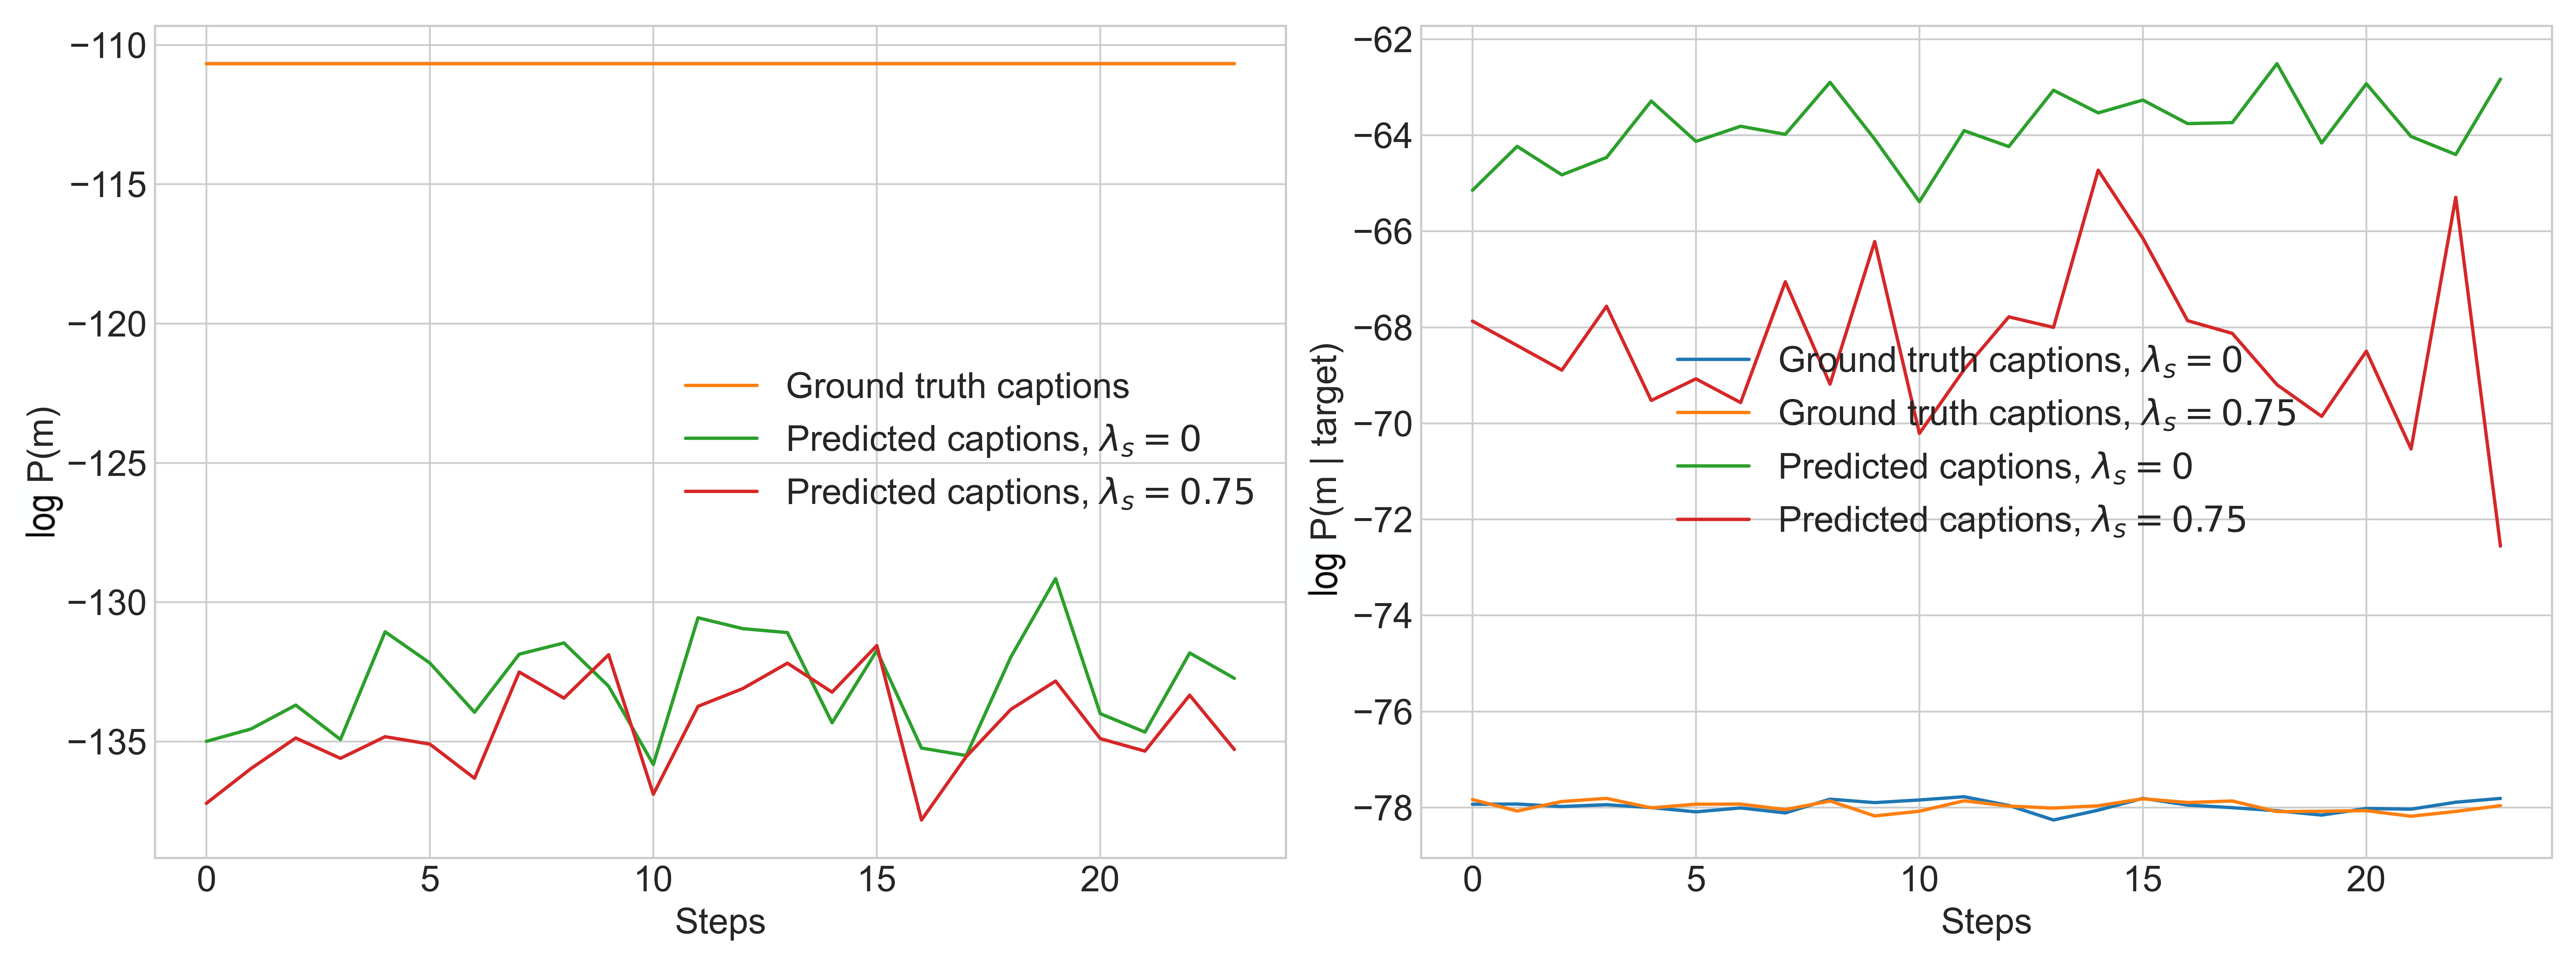
\includegraphics[width=\linewidth]{images/coco_fixedListener_structural_semantic_drift_4000_pure_0_075_random.png}
	\caption{Drift dynamics computed during reference game training with the fixed listener on MS COCO (pure decoding, $\lambda_s=0$ vs. $\lambda_s=0.75$). Higher values indicate less drift. Left: Structural drift of ground truth and predicted captions under the pretrained Transformer XL model. Right: Semantic drift of ground truth and predicted captions under the pretrained speaker model.}
	\label{fig:coco_fixed_listener_075_str_sem_drift}
\end{figure}

In order to investigate whether task improvement can be achieved without speaker-listener co-adaptation when a stronger functional learning signal is present, a second experiment with $\lambda_s=0$ (i..e, functional learning only) was conducted. While no improvement in terms of task performance is apparent visually (Fig,~\ref{fig:coco_fixed_listener_speaker_loss_listener_acc_075}), there was an little increase in terms of listener test accuracy to 0.888 (Tab.~\ref{tab:coco_drift_metrics_basic}). Furthermore, Table \ref{tab:coco_drift_metrics_basic} indicates that under stronger functional constraints, language drift was mitigated even better, compared to the $\lambda_s = 0.75$ fixed listener. More precisely, structural drift was lower, even outperforming the pretrained speaker. Similarly, semantic drift also narrowly improved beyond both the pretrained and the $\lambda_s = 0.75$ speakers. 
The overlap metrics also slightly improved or remained constant compared to both the $\lambda_s=0.75$ experiment, the jointly trained listener-speaker experiment and the pretrained speaker. These results suggest that when removing the agent co-adaptation, a strong enough functional training signal might yield more discriminative captions which mention more target than distractor features. 

To sum up, the data supports \textbf{H5} for the MS COCO experiment, but also strongly suggests that the functional signal available under the functional loss weight of 0.25 is not sufficient in order to visibly fine-tune the speaker for the task. When increasing the strength of the functional signal from the listener by setting $\lambda_s$ to 0, a tangiable improvement of language drift can be observed, indicating that both grounding and the structure expected by the listener positively affect the speaker. \pt{check}.

\subsection{3Dshapes: Baseline Experiments}
\label{expt:3dshapes_baseline}

The goal of these experiments is to investigate the importance of presenting exhaustive example captions to the model during training for potentially mitigating structural drift. Additionally, these experiments focus on investigating the model's potential to generate informative captions, without being overinformative. \pt{spell out the operationalization}

%\begin{sidewaystable}
\begin{table}[] 
	\begin{tabularx}{\textwidth}{|X|l|l|X|X|X|X|}
		\hline
		\textbf{Model name}                                    & \textbf{log $P(m)$} & \textbf{log $P(m \mid i)$} & \textbf{Overlap (d)} & \textbf{Overlap (c)} & \textbf{Listener acc (random)} & \textbf{Listener acc (similar)} \\ \hline
		Ground truth exh.       &      -164.752            &         -101.329               &       6.881             &      0.023               &                 &                \\ \hline
		Pretrained 3D exh. speaker                            &       -195.753            &         -145.638               &        5.428              &      0.001                & 0.953 (random listeners)                 & 0.808 (similar listeners)                 \\ \hline
		3D Baseline, random, $\lambda_s = 0$ &       -195.420            &    -147.938                    &           5.294            &      -0.002                &                 0.979                         &                                           \\ \hline
		3D Baseline, random, $\lambda_s = 0.25$     &     -196.811              &       -140.862                 &          5.104            &       -0.006               &          0.969                                &                                           \\ \hline
		3D Baseline, random, $\lambda_s = 0.5$   &         -196.722          &        -144.301                &        4.968              &          0.002            &                  0.971                      &                                           \\ \hline
		3D Baseline, random, $\lambda_s = 0.75$  &       -195.495        &           -147.313           &          5.247            &         0.001             & 0.979                                    &                        0.959                   \\ \hline
		3D Baseline, random, $\lambda_s = 1$   &      -196.019             &            -137.456             &        5.257              &          -0.005            &              0.979                            &                                           \\ \hline
		3D fixed listener, random, $\lambda_s = 0$&      -196.111          &     -136.134                  &             5.339         &         -0.008            &                   0.927                      &                                           \\ \hline
		3D fixed listener, random, $\lambda_s = 0.75$&      -194.990          &     -140.483                  &             5.298         &         -0.003            &                   0.927                      &                                           \\ \hline
	\end{tabularx}
	\caption{\label{tab:3dshapes_drift_metrics_basic_baseline} Language drift metrics and listener test accuracies on different pairs. 
		``Baseline'' refers to the setup wherein the listener is trained jointly with the speaker, using pure decoding. MS refers to the MS COCO dataset, 3D ro the 3DShapes one. ``Random'' refers to speakers trained on random target-distractor pairs; ``similar'' refers to speakers trained on similar target-distractor pairs. ``Overlap (d)'' refers to the discrete overlap metric, ``overlap (c)'' to continuous overlap. The speakers trained on similar pairs are still tested on random pairs.}
\end{table}
%\end{sidewaystable}


\begin{figure}[h]
	\centering
	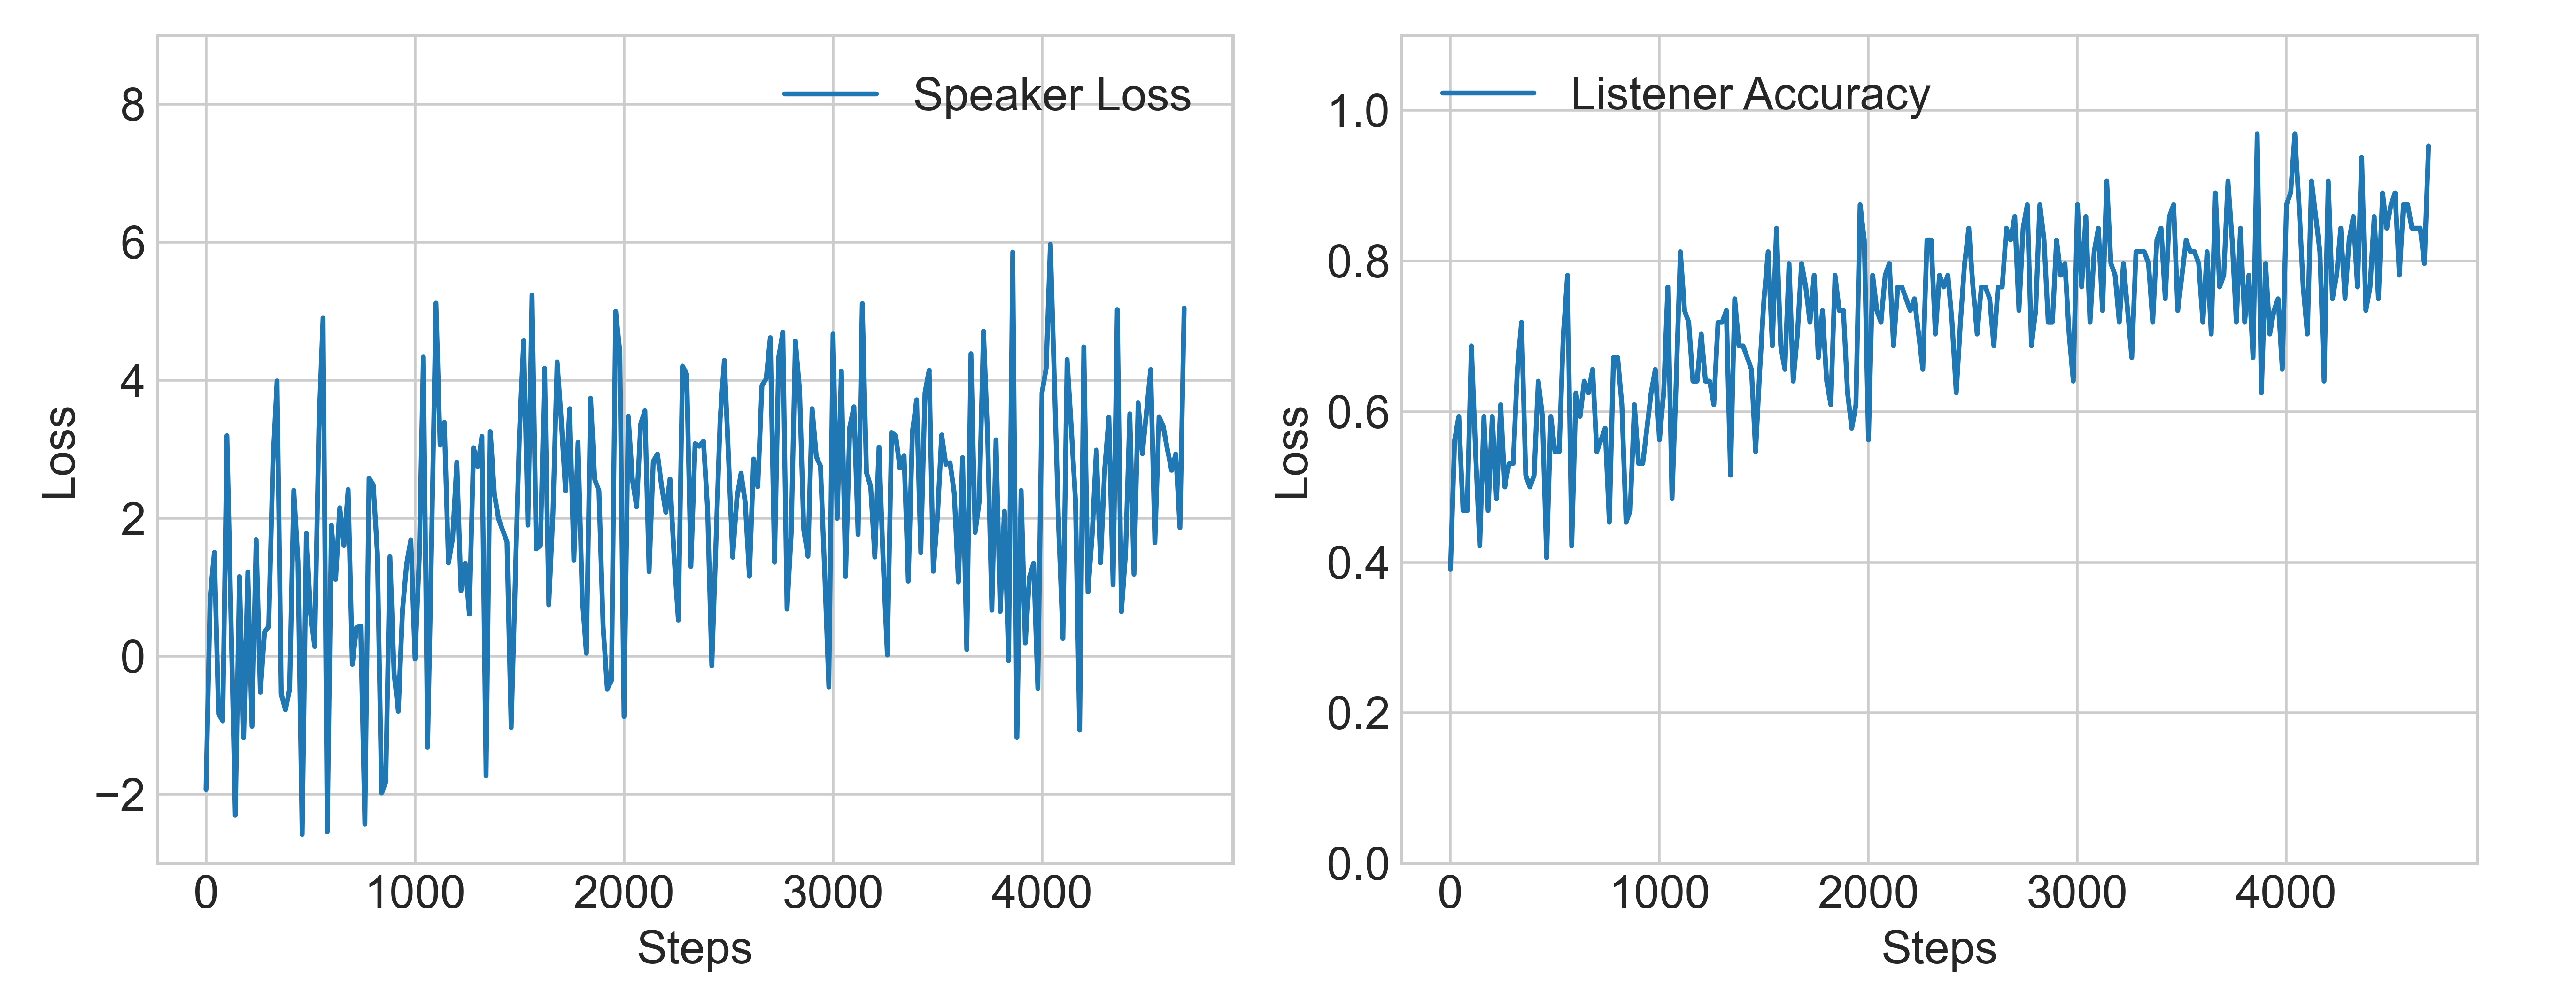
\includegraphics[width=\linewidth]{images/3dshapes_refgame_49_pure_075.png}
	\caption{Training results of the baseline 3Dshapes experiment (pure decoding, $\lambda_s = 0.75$). Left: Total speaker training loss. Right: Listener training accuracy.}
	\label{fig:3dshapes_baseline_075_speaker_loss_listener_acc}
\end{figure}


\begin{figure}
	\centering
	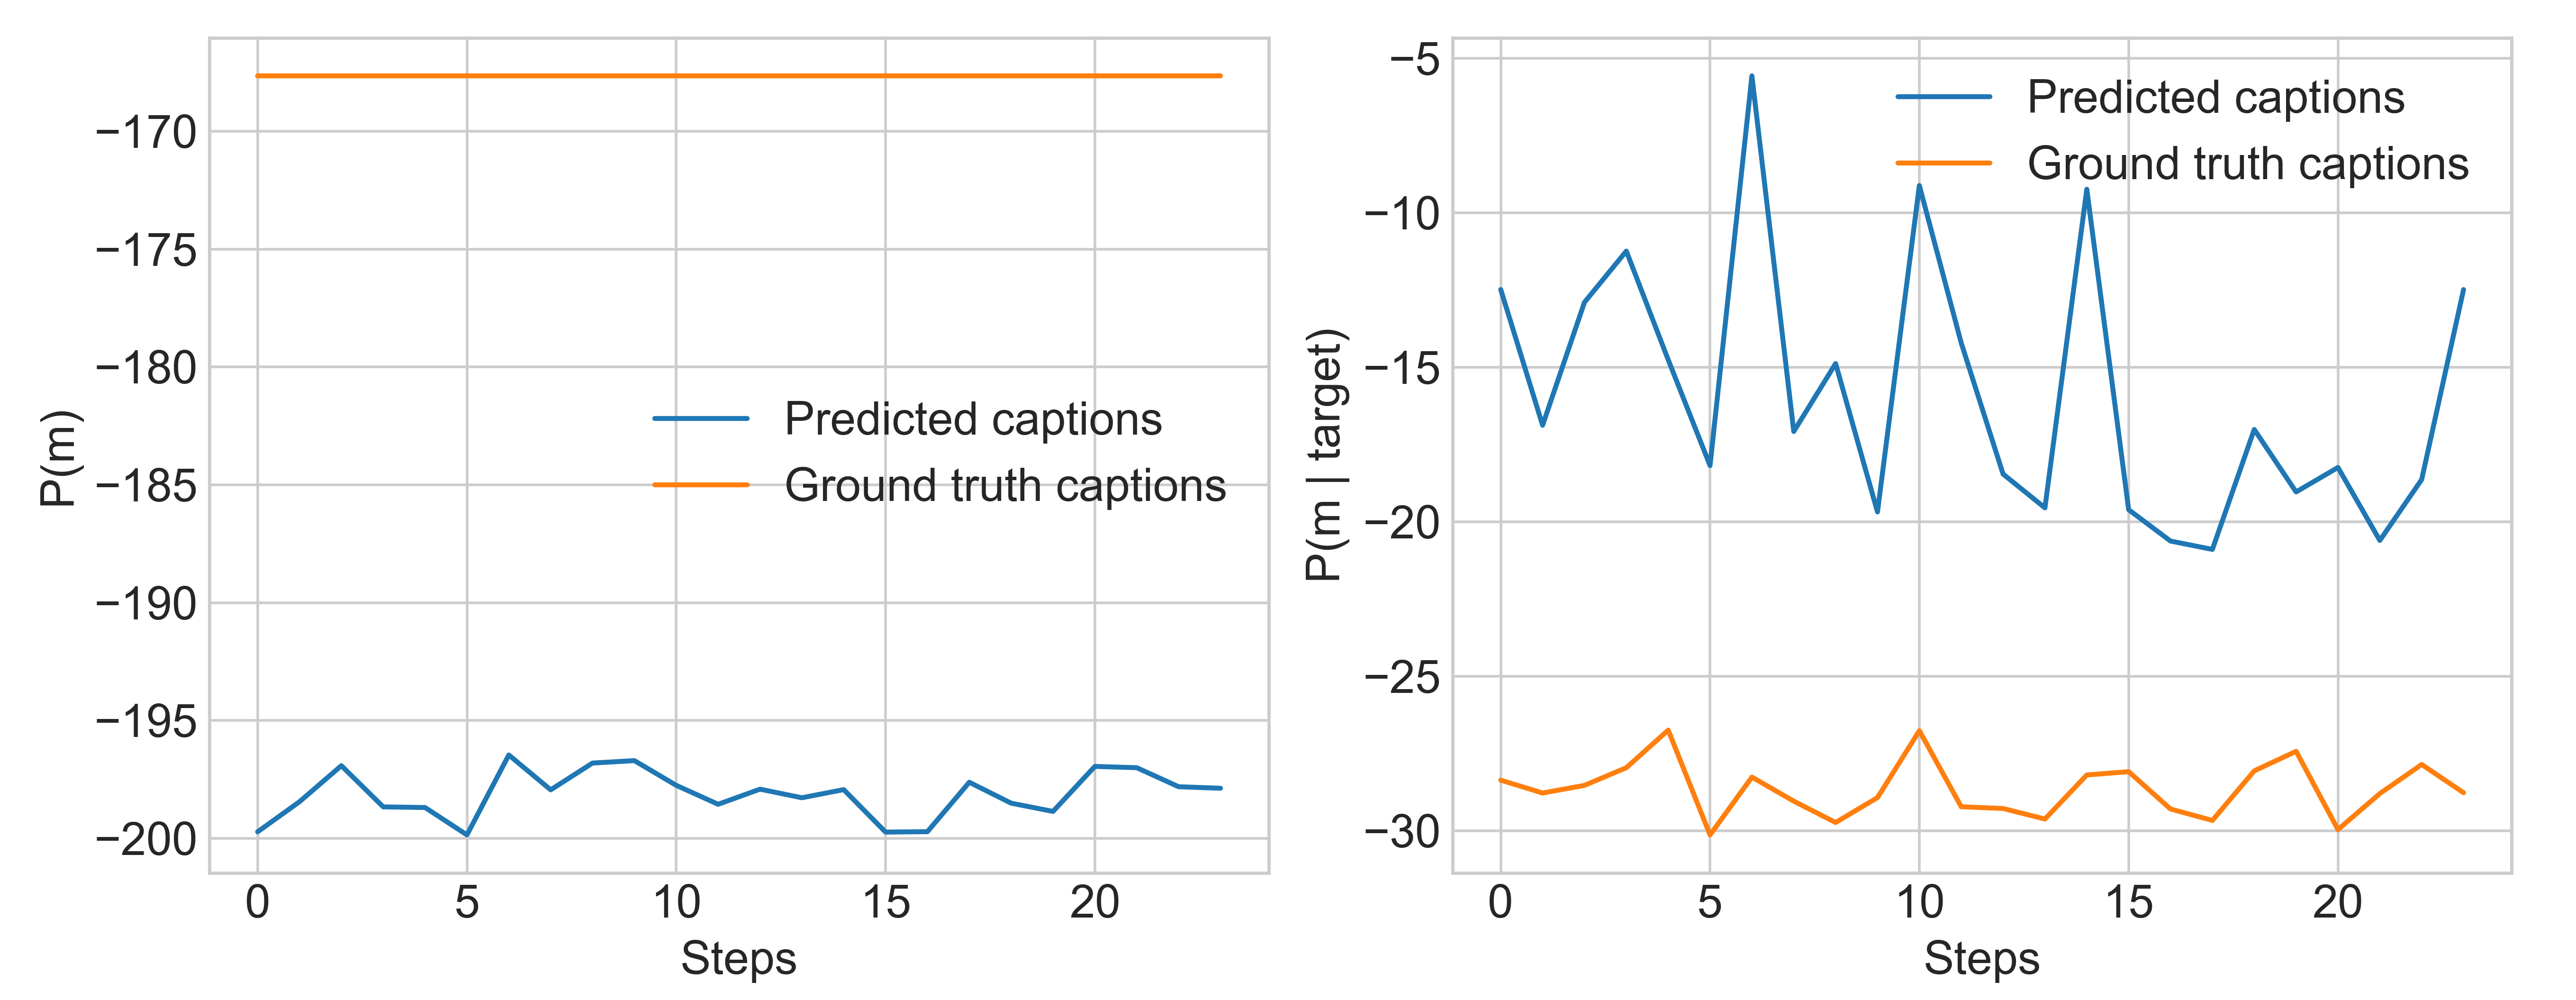
\includegraphics[width=\linewidth]{images/3dshapes_structural_semantic_drift_49_pure_075_random.png}
	\caption{Drift computed every 200 training steps on 50 images in the baseline 3Dshapes experiment (pure decoding, $\lambda_s = 0.75$). Higher values are better. Left: Strucutral drift of ground truth and predicted captions. Right: Semantic drift of ground truth and predicted captions under the pretrained speaker model.} 
	\label{fig:3dshapes_baseline_075_str_drift}
\end{figure}

The configurations as well as the training procedure of this experiment match the configurations of the MS COCO baseline experiment in Section \ref{expt:coco_baseline}. The training dynamics of the baseline experiment with $\lambda_s = 0.75$ can be seen in Figure \ref{fig:3dshapes_baseline_075_speaker_loss_listener_acc}. Interestingly, compared to the reference game on MS COCO (see Fig.~\ref{fig:coco_baseline_075_speaker_loss_listener_acc}, right), the training of the listener does not visibly converge faster, although the action space (i.e., vocabulary space---49 tokens for 3Dshapes vs. 4052 tokens for MS COCO) that the speaker has to explore is significantly smaller. 
 
Supporting the visual results, Table \ref{tab:3dshapes_drift_metrics_basic} shows that the agents successfully learned the reference game---the listener test accuracy is 0.979, even outperforming the MS COCO baseline experiment. Performance also improved by 0.026 compared to the pretrained speaker. 
Supporting \textbf{H2}, slight semantic drift can be observed in this experiment---the average conditional log likelihood of the captions generated by the trained speaker decreased by 1.675, compared to the captions produced by the pretrained speaker. Interestingly, in contrast to the MS COCO baseline experiment, \textbf{H1} is not supported in this experiment, as the average log likelihood under the pretrained LM actually increased by 0.258 for the captions of the baseline experiment speaker, compared to the pretrained one (Table~\ref{tab:3dshapes_drift_metrics_basic}).
 
The dynamics of structural and semantic drifts can be seen in Figure \ref{fig:3dshapes_baseline_075_str_drift}; these are in line with the validation results.\footnote{Due to a coding mistake, the language drift and validation loss computed during training of the baseline random pairs experiment on 3Dshapes were computed on 50 images from the training dataset, not the validation dataset. Furthermore, semantic drift was computed using greedy decoding, and only on one image pair.} 
Interestingly, the magnitude of the structural drift values is much higher for 3Dshapes, indicating that the created captions might in general be less likely under the pretrained Transformer XL model used for the computation. Similarly, the higher magnitude of the semantic drift values indicates that the speaker is generally uncertain when generating captions for these images. This could partly be due to the difference in the 3Dshapes data distribution compared to the ImageNet data in which the visual module of the speaker was pretrained. Additionally, this could be due to the variability of the syntactic structure of the ground truth sentences. 

Turning to the overlap metrics in Table~\ref{tab:3dshapes_drift_metrics_basic}, the discrete overlap decreased by 0.181 tokens on average, compared to the pretrained speaker. Similarly to MS COCO, the overlap is also generally lower than for the ground truth captions, indicating that the trained speaker's captions might not cover all features mentioned in the exhaustive ground truth captions. An interesting direction for future work is the investigation of potential regularities in the type of feature descriptions omitted by the speaker. A further interesting observation is that the difference in the discrete overlaps between the baseline speaker and the ground truth captions is much smaller in the 3Dshapes experiment (1.634), compared to MS COCO (7.95). This might be an indication of a more robust grounding of the 3Dshapes speaker mentioning more of the features contained in the images, compared to the MS COCO speaker, which might be attributed to the significantly smaller action space of the former. In sum, \textbf{H3} is not supported by the data from the 3Dshapes experiment.

\pt{Linear regressions will be computed on the drift values collected during the training.}

Additionally, the fine-tuned speaker was also evaluated with standard image captioning metrics. Table \ref{tab:eval_metrics_refgame} shows that caption quality marginally decreased with respect to almost all metrics except for CIDEr and BLEU-1. Noteworthily, in contrast to the language drift metrics, these metrics are significantly higher for the 3Dshapes dataset compared to MS COCO, indicating that the generated captions have a relatively high overlap with ground truth captions. This calls for careful consideration of the pretraining datasets and their similarity to the target dataset when using available pretrained models like ResNet and Transformer XL.

\subsubsection{Varying Structural Loss}

\begin{figure}
	\centering
	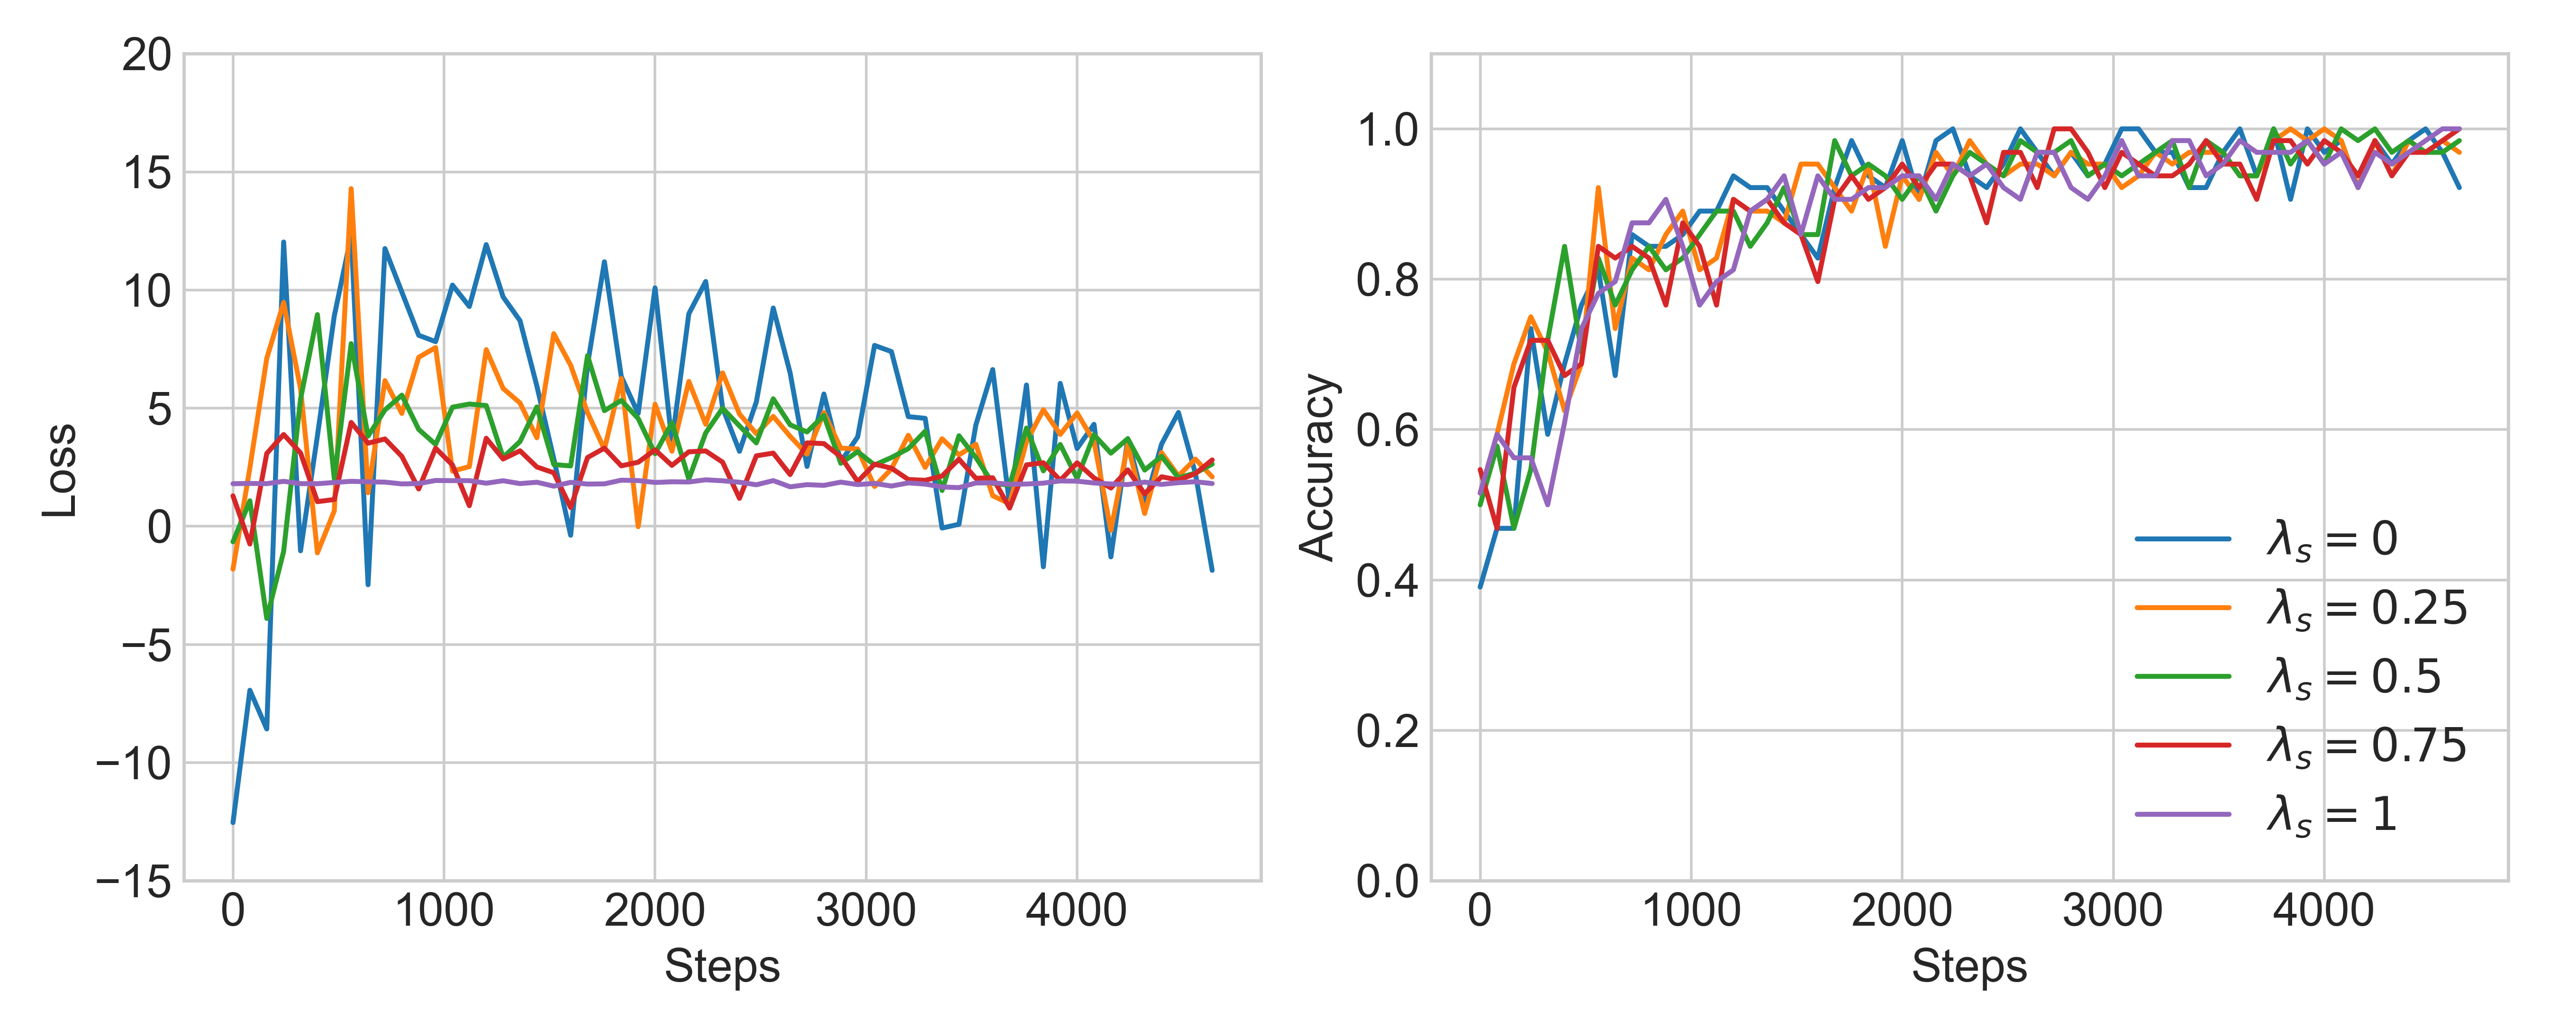
\includegraphics[width=\linewidth]{images/shapes_refgame_49_pure_losses_all_Ls_random.png}
	\caption{Training results of the 3Dshapes experiment with varying $\lambda_s$ (pure decoding). Left: Total speaker train loss. Right: Listener train accuracy.}
	\label{fig:3dshapes_baseline_speaker_loss_listener_acc_all}
\end{figure}


\begin{figure}
	\centering
	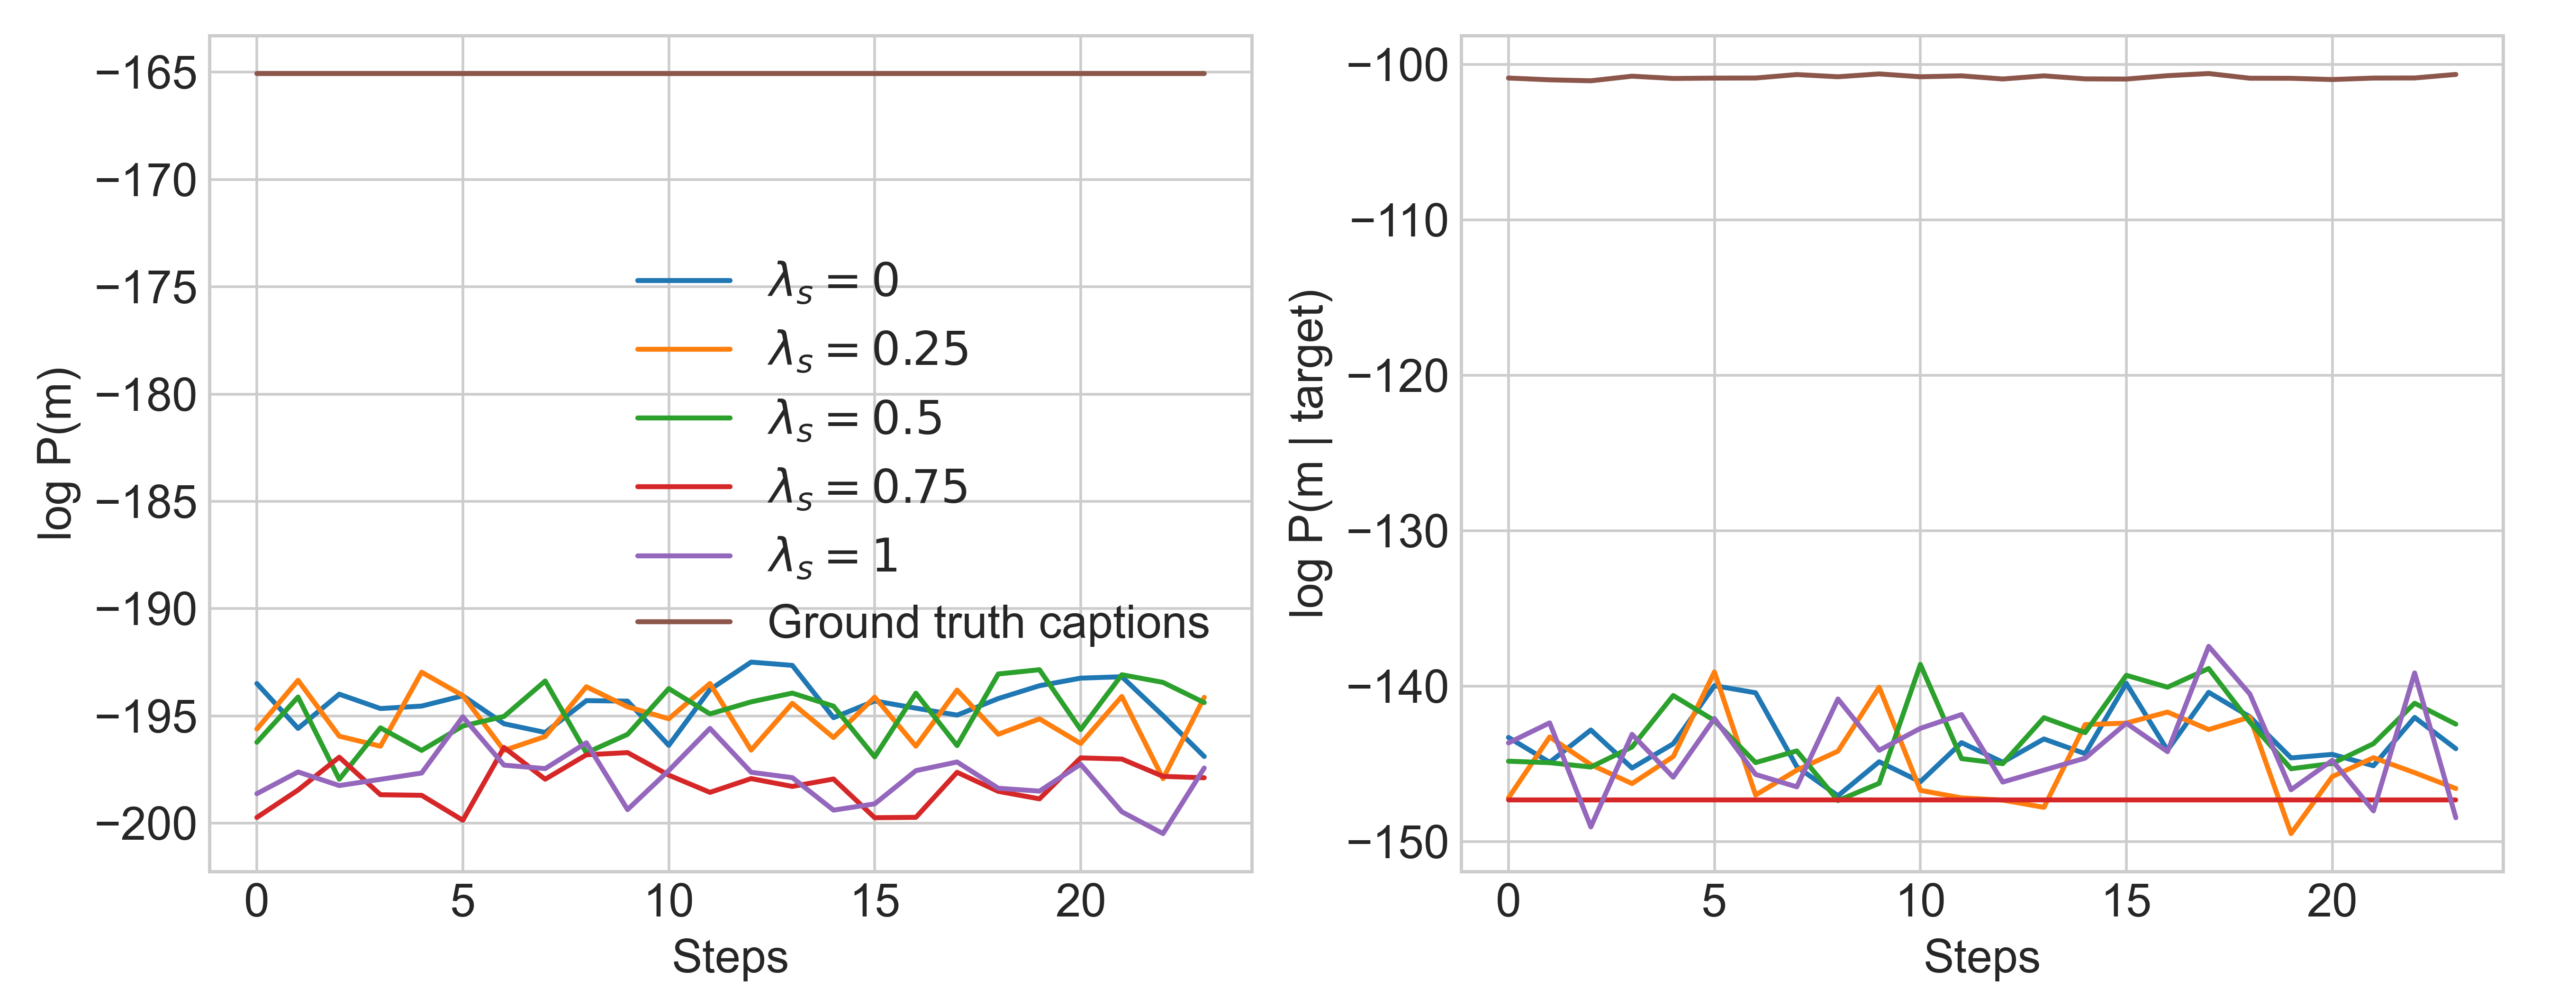
\includegraphics[width=\linewidth]{images/shapes_structural_semantic_drift_49_pure_L_s_all_random.png}
	\caption{Drift metrics computed every 200 training steps on 192 images in the baseline 3Dshapes experiments, across $\lambda_s$ values. Higher values indicate less drift. Left: Strucutral drift of ground truth and predicted captions. Right: Semantic drift of ground truth and predicted captions under the pretrained speaker model. The drift is constant for $\lambda_s = 0.75$ due to a coding error, it is the mean validation drift from Table \ref{tab:3dshapes_drift_metrics_basic}.} 
	\label{fig:3dshapes_baseline_all_str_sem_drift}
\end{figure}

In order to adress \textbf{H4} with the 3Dshapes dataset, a line of experiments identical to MS COCO based ones were conducted. Specifically, the structural loss weight $\lambda_s$ was also varied. The pattern of results visible in Figure~\ref{fig:3dshapes_baseline_speaker_loss_listener_acc_all} is very similar to MS COCO. The magnitude of the speaker loss is what is mostly influenced by the $\lambda_s$ weight; the listener's training accuracy is not affected by the variation. This is confirmed by the consistently high listener test accuracy, outperforming the pretrained speaker (Table~\ref{tab:3dshapes_drift_metrics_basic}, fifth column). Differently to MS COCO, the speaker trained with $\lambda_s = 1$ outperformed the pretrained speaker by 0.026, indicating that there might have been room for further pretraining of the speaker. \pt{be careful to not confuse task performance with pretraining; also check this in coco.}

As for MS COCO, validation language drift metrics were computed on a held out validation set of 1000 images. Table \ref{tab:3dshapes_drift_metrics_basic} indicates that, similarly to MS COCO, no clear trends can be observed with respect to all four drift metrics. Negative continuous overlap values (Tab.~\ref{tab:3dshapes_drift_metrics_basic}, fourth column) indicate that the emebddings of generated captions were partly more similar to the distractor ground truth embeddings, than to target ground truth embeddings. These findings are generally corroborated by the dynamics of structural and semantic drifts computed during training (see Fig.~\ref{fig:3dshapes_baseline_all_str_sem_drift}). In contrast to MS COCO, semantic drift of the captions produced by the speakers is stronger than of the ground truth captions, i.e., the conditional log likelihood of the generated captions is lower. 

These speakers were also evaluated on the image captioning metrics. \pt{TODO Table \ref{tab:eval_metrics_refgame} indicates that the captions for all $\lambda_s$ configurations are closer to ground truth captions compared to MS COCO results.}

These experiments in comparison to analogous experiments on MS COCO (Section \ref{expt:coco_baseline}) also allowed to adress \textbf{H9} as they provide different degrees of freedom for the model to exploit structural deterioration as a method for producing `more discrminative' captions. In line with \textbf{H9}, the largest difference in structural drift compared to the pretrained speaker in 3Dshapes experiments on random image pairs is 1.058 (Tab.~\ref{tab:3dshapes_drift_metrics_basic}), compared to 5.164 (Tab.~\ref{tab:coco_drift_metrics_basic}). 

To sum up, similarly to MS COCO, the precise parametrization of the loss did not consistently influence task performance or language drift, given the model and the dataset.

\subsection{3Dshapes: Similar Pairs Experiments}
\label{expt:3dsapes_similar}

\begin{table}[] 
	\begin{tabularx}{\textwidth}{|X|l|l|X|X|X|X|}
		\hline
		\textbf{Model name}                                    & \textbf{log $P(m)$} & \textbf{log $P(m \mid i)$} & \textbf{Overlap (d)} & \textbf{Overlap (c)} & \textbf{Listener acc (random)} & \textbf{Listener acc (similar)} \\ \hline
		Ground truth exh.       &      -164.752            &         -101.329               &       6.881             &      0.023               &                 &                \\ \hline
		Pretrained 3D exh. speaker                            &       -195.753            &         -145.638               &        5.428              &      0.001                & 0.953 (random listeners)                 & 0.808 (similar listeners)                 \\ \hline
		3D Baseline, random, $\lambda_s = 0.75$  &       -195.495        &           -147.313           &          5.247            &         0.001             & 0.979                                    &                        0.959                   \\ \hline
		3D Baseline, similar, $\lambda_s = 0.75$ &      -198.189             &       -140.786                 &           5.578           &        0.001              & 0.878                      &            0.906                        \\ \hline
		3D Baseline, similar fixed, same test, $\lambda_s = 0.75$ &       -193.709            &    -141.010                  &        3.280            &      -0.003         &            0.688       &                              \\ \hline
		3D Baseline, similar fixed, diff. test, $\lambda_s = 0.75$ &      -193.524             &          -144.813            &       3.230             &     -0.005          &     0.711              &                              \\ \hline
		3D Short, similar, $\lambda_s = 0.75$&      -145.014             &      -76.474                  &             1.565         &         0.000             &                   0.885                       &                                           \\ \hline
		3D Short, similar fixed, same test $\lambda_s = 0.75$&      -190.010           &     -58.128                  &             2.086         &         0.001             &                   0.731                       &                                           \\ \hline
		3D Short, similar fixed, diff. test $\lambda_s = 0.75$&     -191.051        &        -59.088           &   1.947        &        0.002          &        0.717                               &                                           \\ \hline
	\end{tabularx}
	\caption{\label{tab:3dshapes_drift_metrics_basic_similar} Language drift metrics and listener test accuracies on different pairs. 
		``Baseline'' refers to the setup wherein the listener is trained jointly with the speaker, using pure decoding. MS refers to the MS COCO dataset, 3D ro the 3DShapes one. ``Random'' refers to speakers trained on random target-distractor pairs; ``similar'' refers to speakers trained on similar target-distractor pairs. ``Overlap (d)'' refers to the discrete overlap metric, ``overlap (c)'' to continuous overlap. The speakers trained on similar pairs are still tested on random pairs.}
\end{table}

\textbf{H5}

\begin{figure}
	\centering
	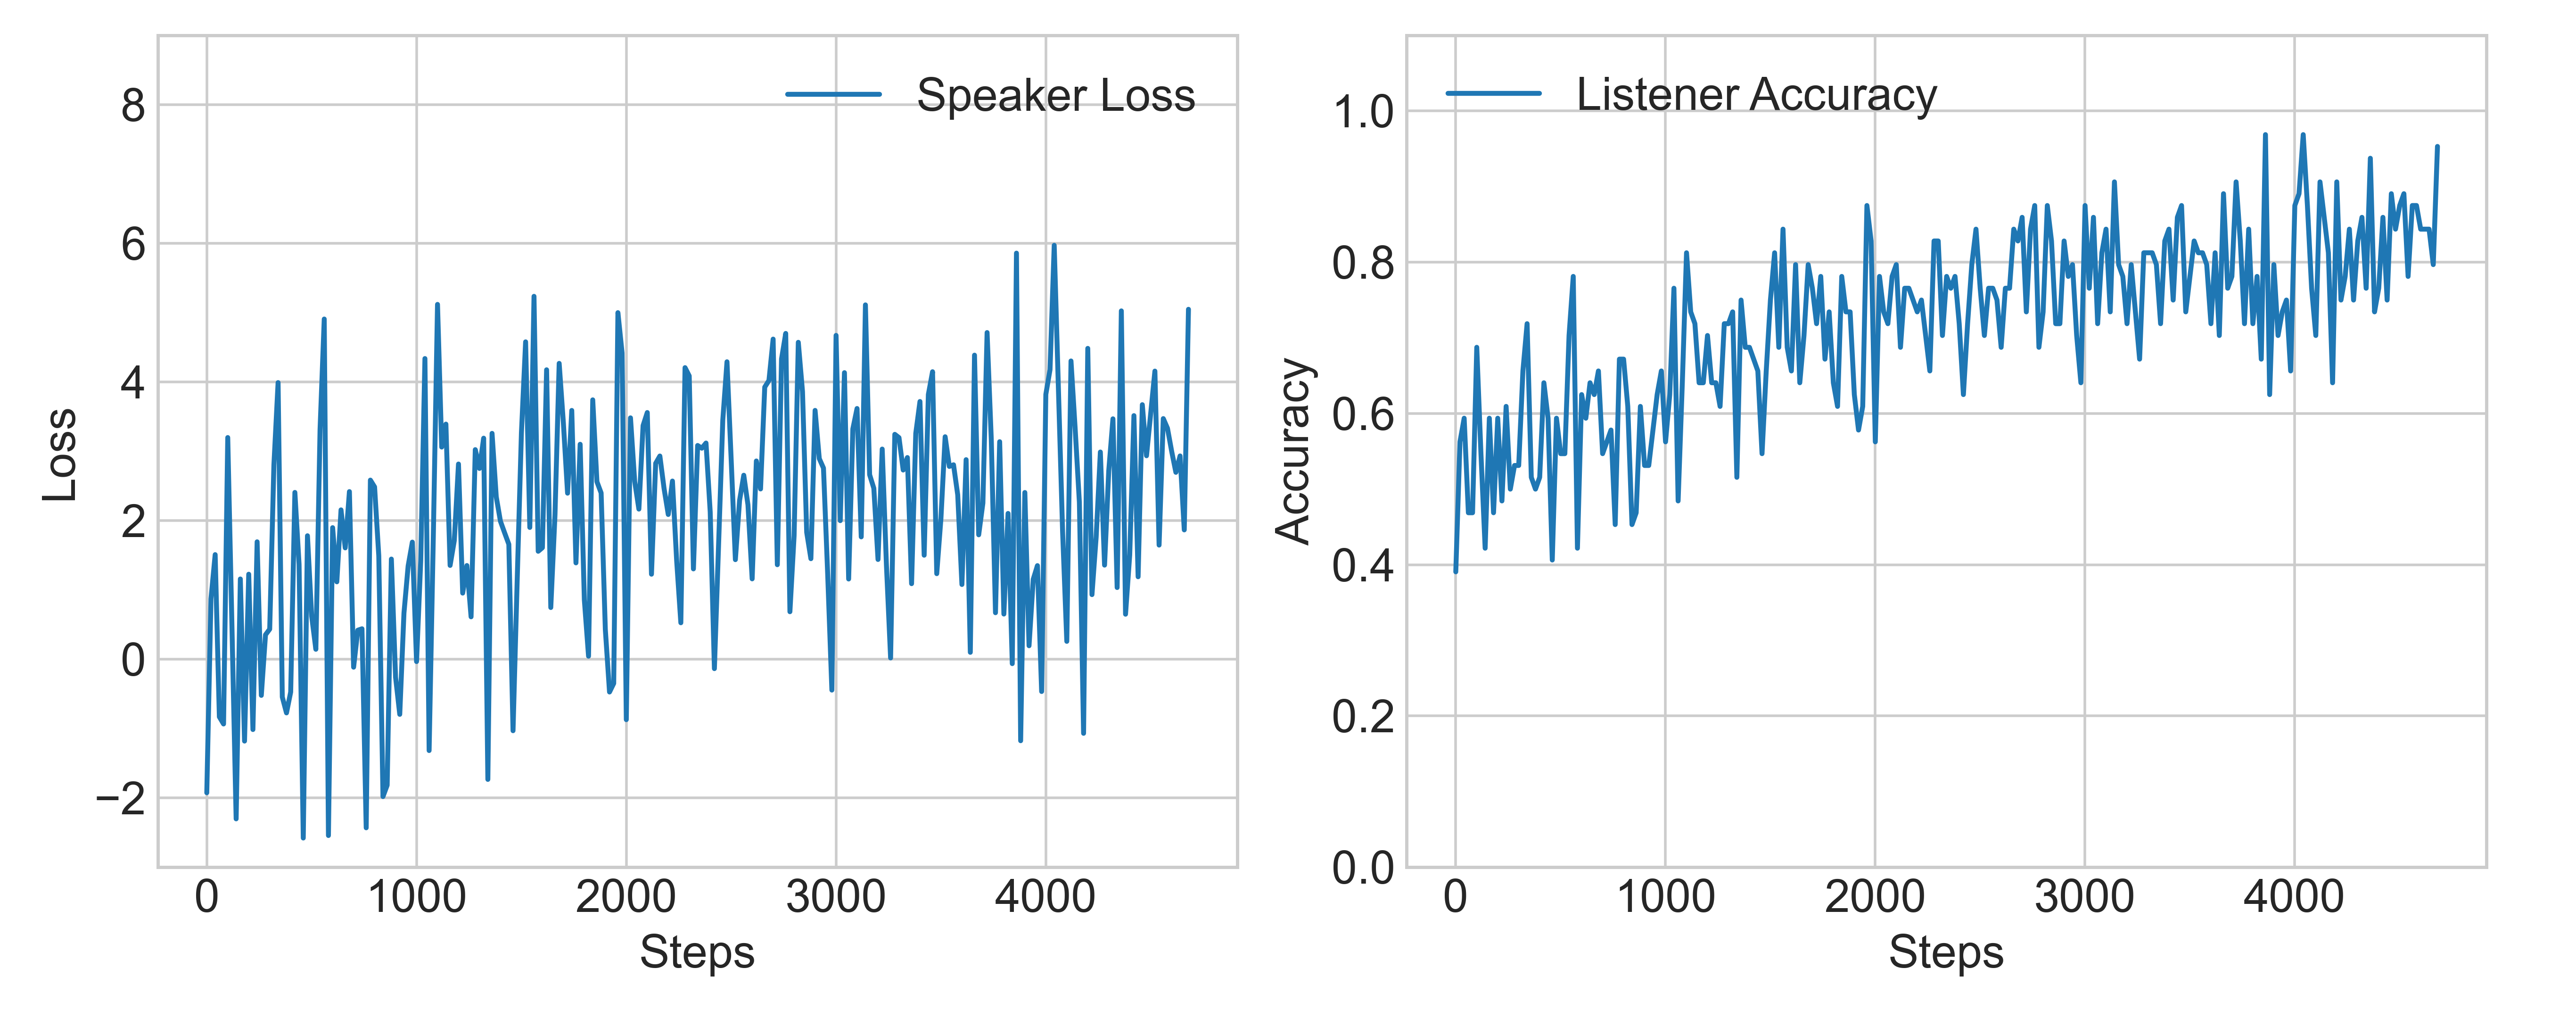
\includegraphics[width=\linewidth]{images/3dshapes_refgame_49_pure_075_similar.png}
	\caption{Training results of the 3Dshapes experiment on similar image pairs (pure decoding, $L_s = 0.75$). Left: Total speaker train loss. Right: Listener train accuracy.}
	\label{fig:3dshapes_similar_075_speaker_loss_listener_acc}
\end{figure}


\begin{figure}
	\centering
	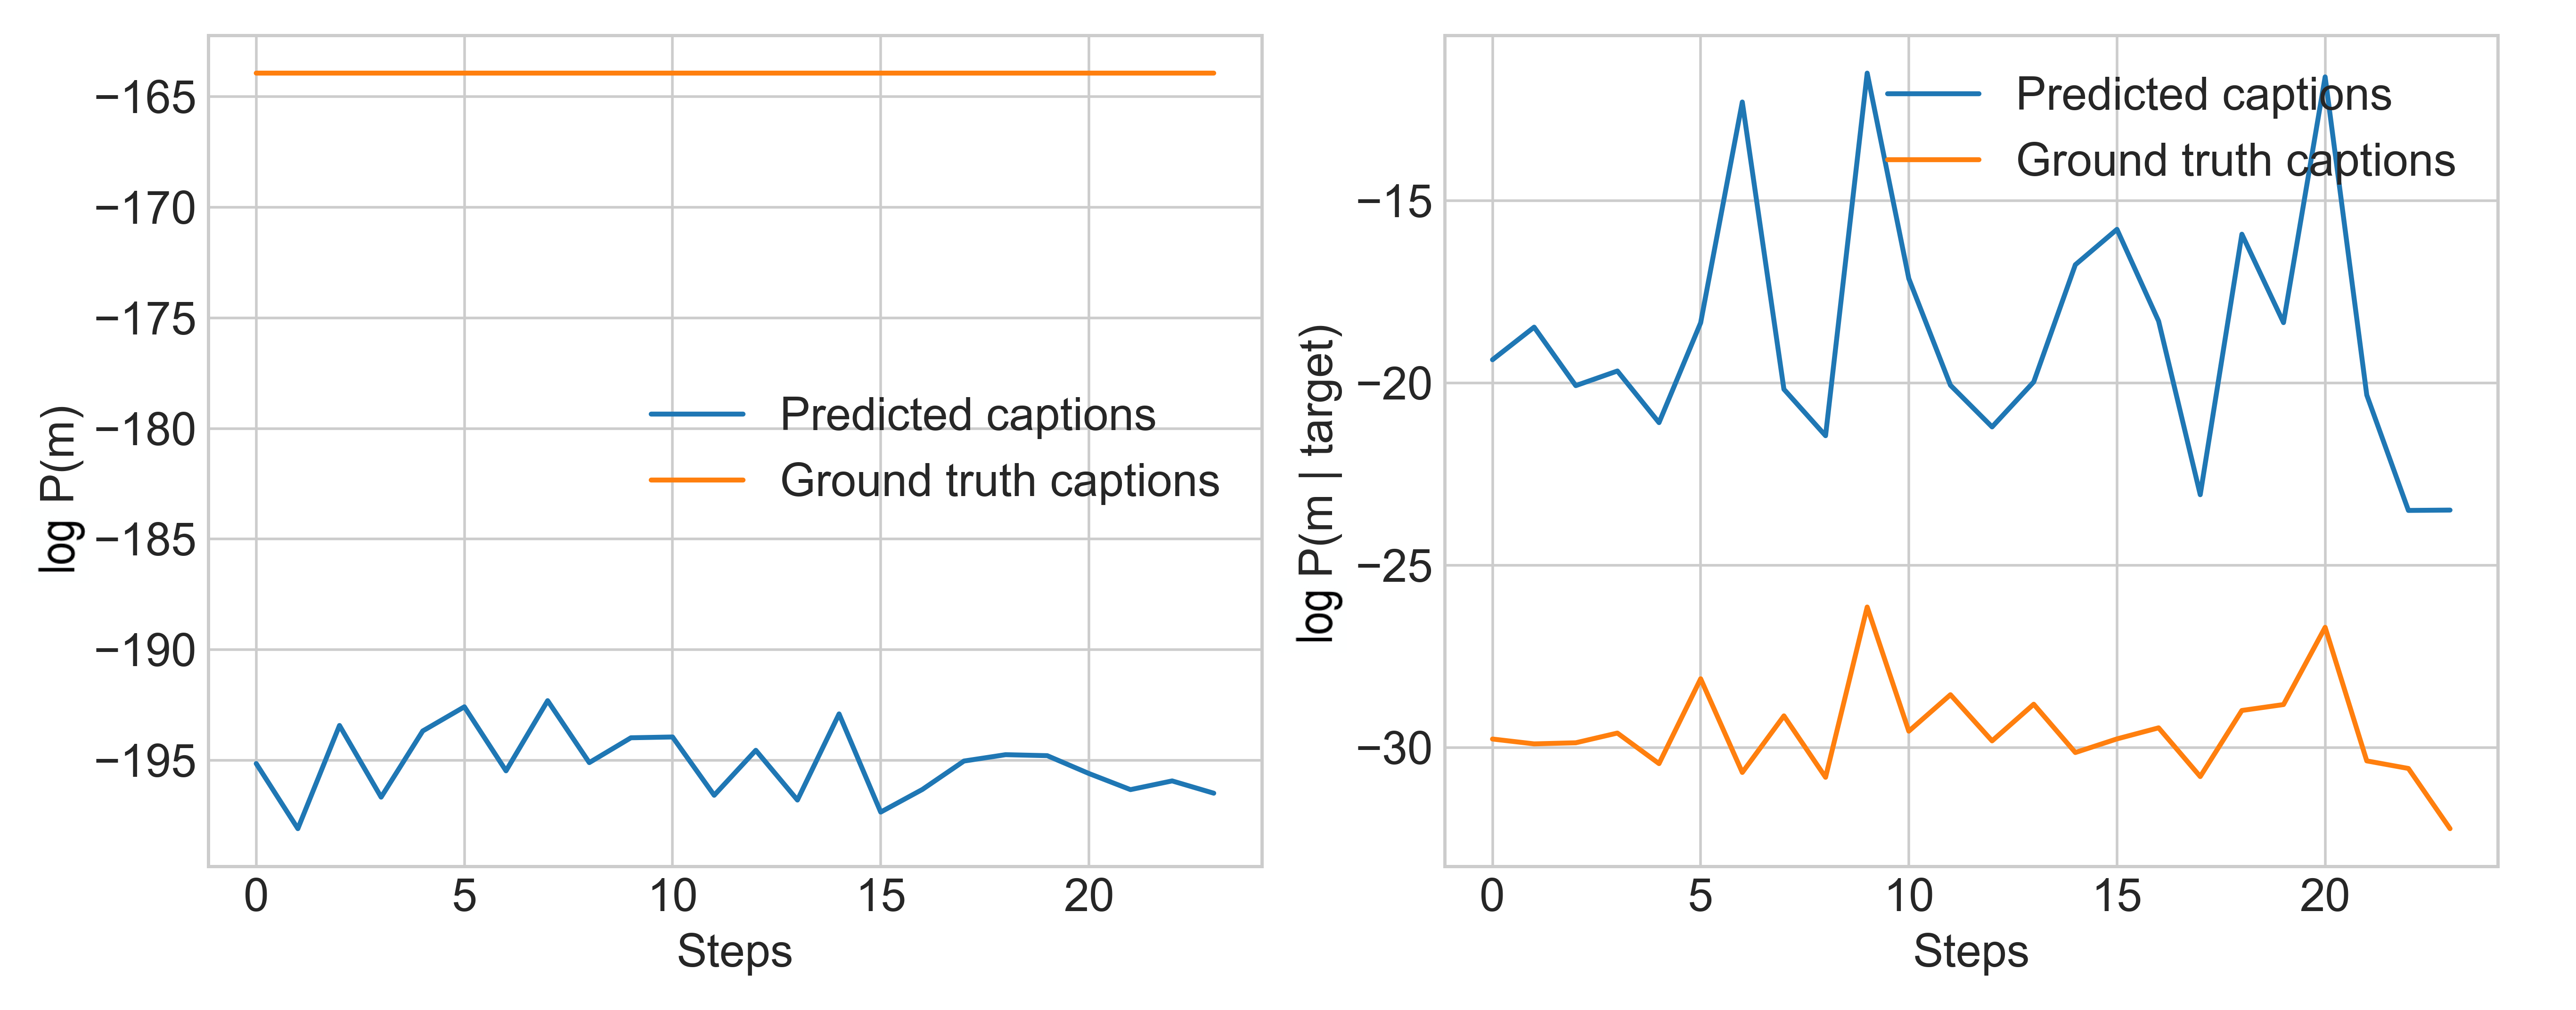
\includegraphics[width=\linewidth]{images/3dshapes_structural_semantic_drift_4000_pure_075_similar.png}
	\caption{Drift computed every 200 training steps on 50 images in the similar image pairs of the 3Dshapes experiment (pure decoding, $L_s = 0.75$). Higher values are better. Left: Structural drift of ground truth and predicted captions. Right: Semantic drift of ground truth and predicted captions under the model pretrained on similar image pairs.} 
	\label{fig:3dshapes_similar_075_str_sem_drift}
\end{figure}

In this experiment, the target-distractor pairs consisted of similar images. That is, at least three of the six features selected at random matched in the target and distractor image. Otherwise, the procedure and configurations are the same as in the baseline experiment in Section \ref{expt:3dshapes_baseline}. 
Figure \ref{fig:3dshapes_similar_075_speaker_loss_listener_acc} (left) indicates that it is much harder for the speaker to produce discriminative messages when the target-distractor pairs are similar, compared to random pairs (Fig.~\ref{fig:3dshapes_baseline_075_speaker_loss_listener_acc}). There are less options for producing good messages, such that the functional reward signal is much weaker than in the former experiment, resulting in almost absent speaker adaptation. Similarly, the listener is much slower to learn the reference game and the grounding of the speaker's messages to the images (Figure \ref{fig:3dshapes_similar_075_speaker_loss_listener_acc}, right). These dynamics confirm that the agents are sensitive to their visual input, and that the task success is closely dependent on the perceptual difficulty to discriminate the target and distractors.

The hypothesis addressed in this experiment is whether the agents were able to flexibly adapt the specificity of their messages, compared to the random pairs baseline experiment (\textbf{H5}). This was approximately investigated via the distribution of part-of-speech tags in a test set of 1000 target-distractor pairs for which messages were generated. The distributions were compared when the 1000 pairs are random versus similar. The results are shown in Figure \ref{fig:3dshapes_pos}. Based on visual inspection, it can be seen that the distribution of the token categories, especially the modifier tokens like color or size adjectives, did not shift significantly. This suggests that the artificial speaker agent is not as flexible in adapting her messages to differences in the input as human speakers (cf. Chapter \ref{chapter03}). However, it is evident from Figure \ref{fig:3dshapes_similar_075_speaker_loss_listener_acc} that the agents did not converge after two epochs, so longer training might provide a different picture. \pt{TODO: compare this with findings by \cite{lazaridou2016multi} and \cite{lee2019countering}.}

\begin{figure}
	\centering
	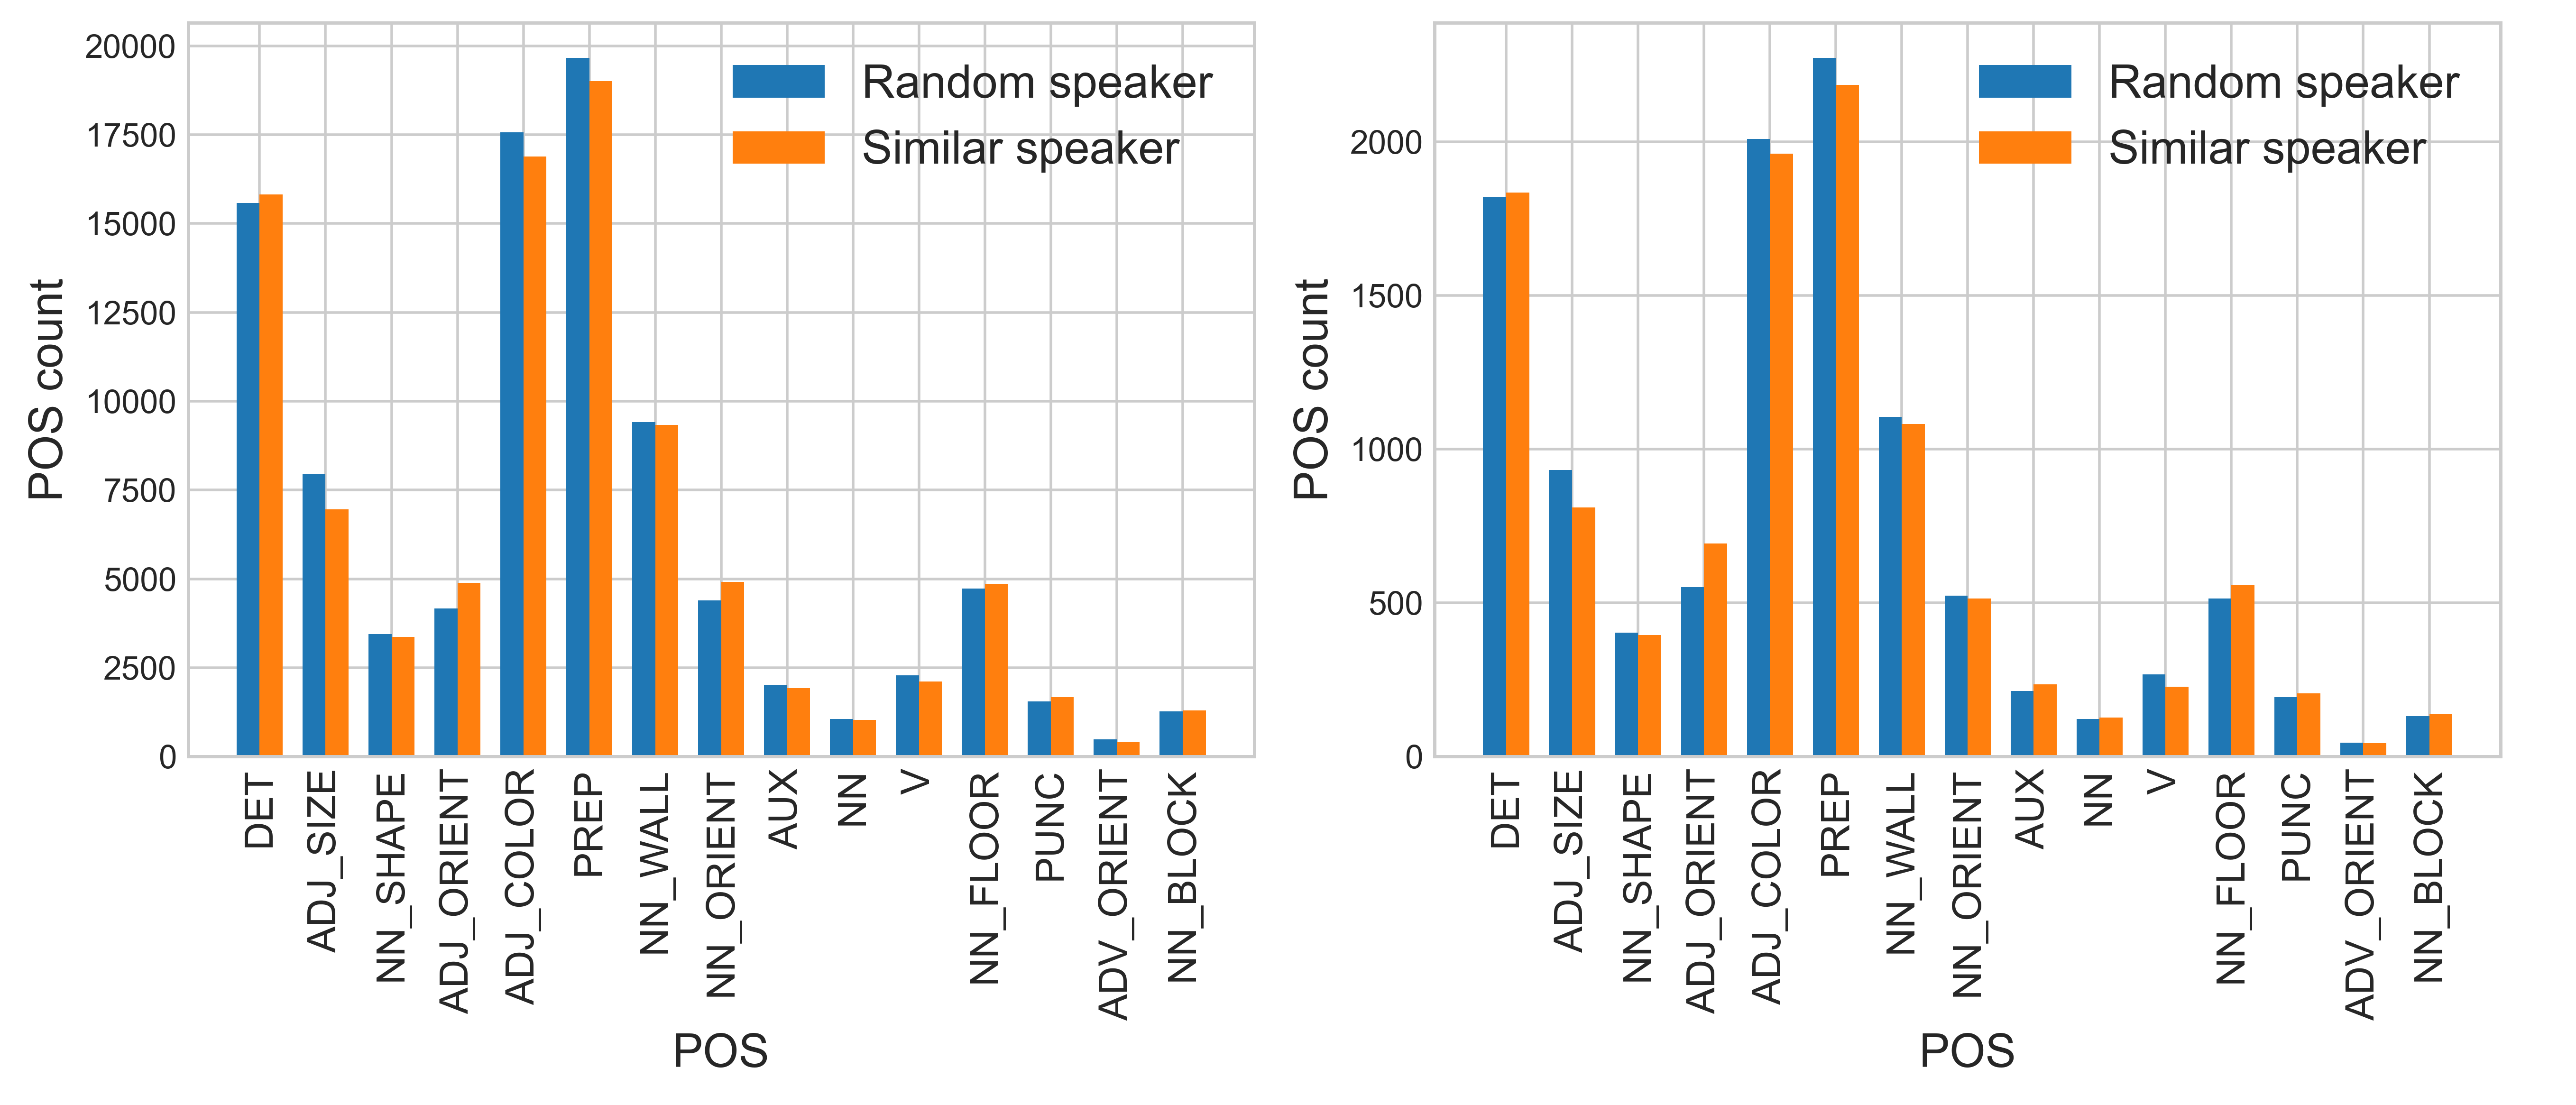
\includegraphics[width=\linewidth]{images/3dshapes_random_vs_similar_POS_counts.png}
	\caption{Left: POS counts in captions produced by a speaker trained on random pairs (blue) and a speaker trained on similar pairs(orange) for 1000 random test image pairs. Right: POS counts in captions produced by a speaker trained on random pairs (blue) and a speaker trained on similar pairs(orange) for 100 similar test image pairs. \pt{The difference in the number of pairs will be fixed}}
	\label{fig:3dshapes_pos}
\end{figure}

In this experiment, structural drift compared to both the pretrained speaker and the baseline experiment can be observed (see Table \ref{tab:drift_metrics_basic}), which is corroborated by a slight visually apparent trend in Figure \ref{fig:3dshapes_similar_075_str_sem_drift}. However, a little increase in the discrete overlap compared to the pretrained speaker indicates that the speaker improved on the task of producing more discriminative messages.
\pt{Check and add summary regarding the hypothesis.}

In order to investigate effects of visual pair similarity in more detail, a follow-up expriment was conducted wherein the features along which the target and the distractor matched were fixed. These features were the object type (cube, ball, pill or cylinder), the object color and the background color. The selection of these features for bein fixed was rather arbitrary, and follow-up experiments should address the visual discriminability of different features more systematically. The training results can be seen in Figure~\ref{3dshapes_similarFixed_075_speaker_loss_listener_acc}.

\begin{figure}
	\centering
	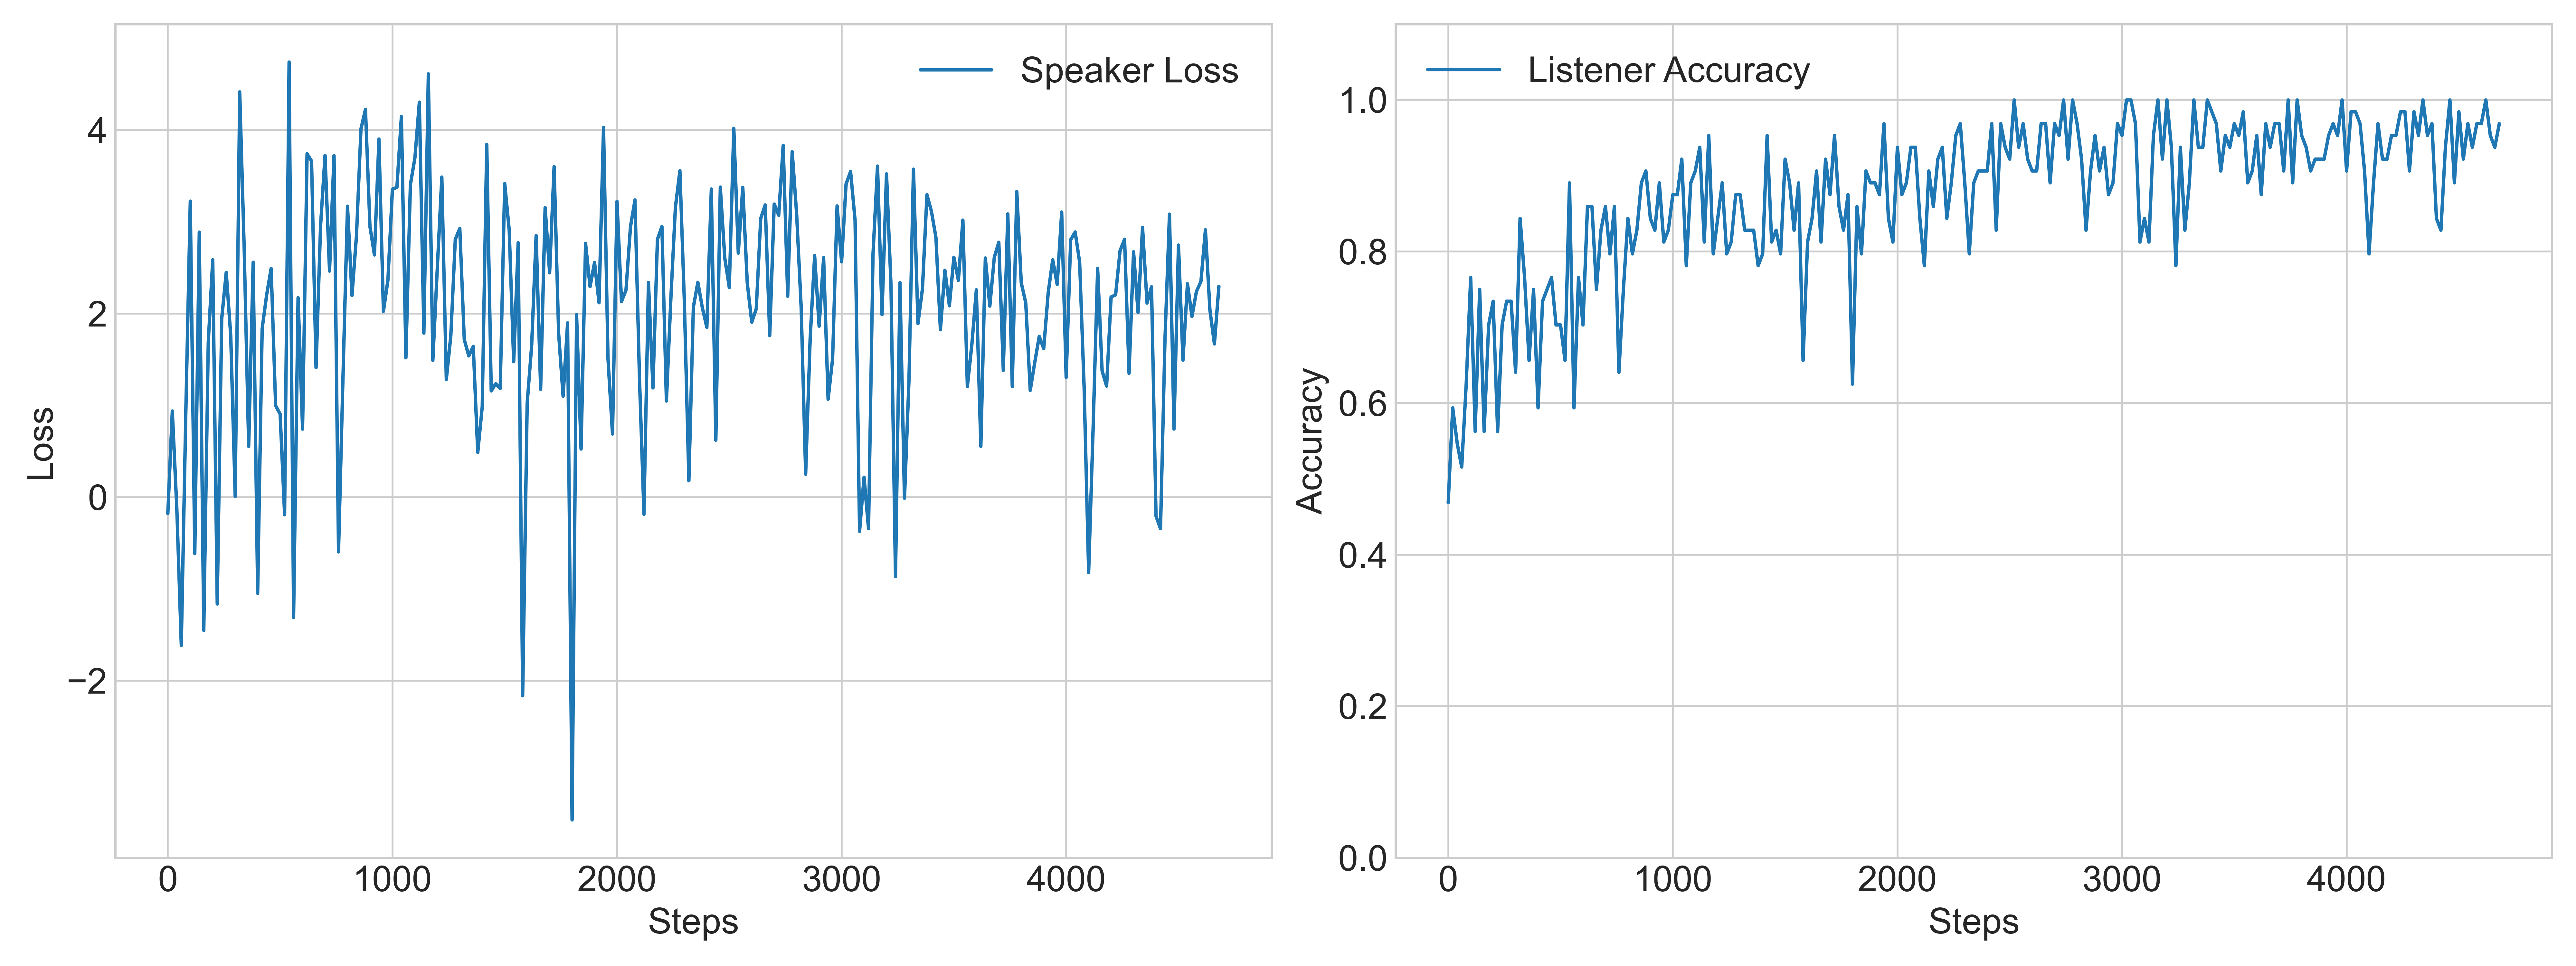
\includegraphics[width=\linewidth]{images/3dshapes_baseline_similarFixed_075_losses.png}
	\caption{Training results of the 3Dshapes experiment on similar image pairs with fixed matching features (pure decoding, $L_s = 0.75$). Left: Total speaker trainining loss. Right: Listener train accuracy.}
	\label{fig:3dshapes_similarFixed_075_speaker_loss_listener_acc}
\end{figure}

\begin{figure}
	\centering
	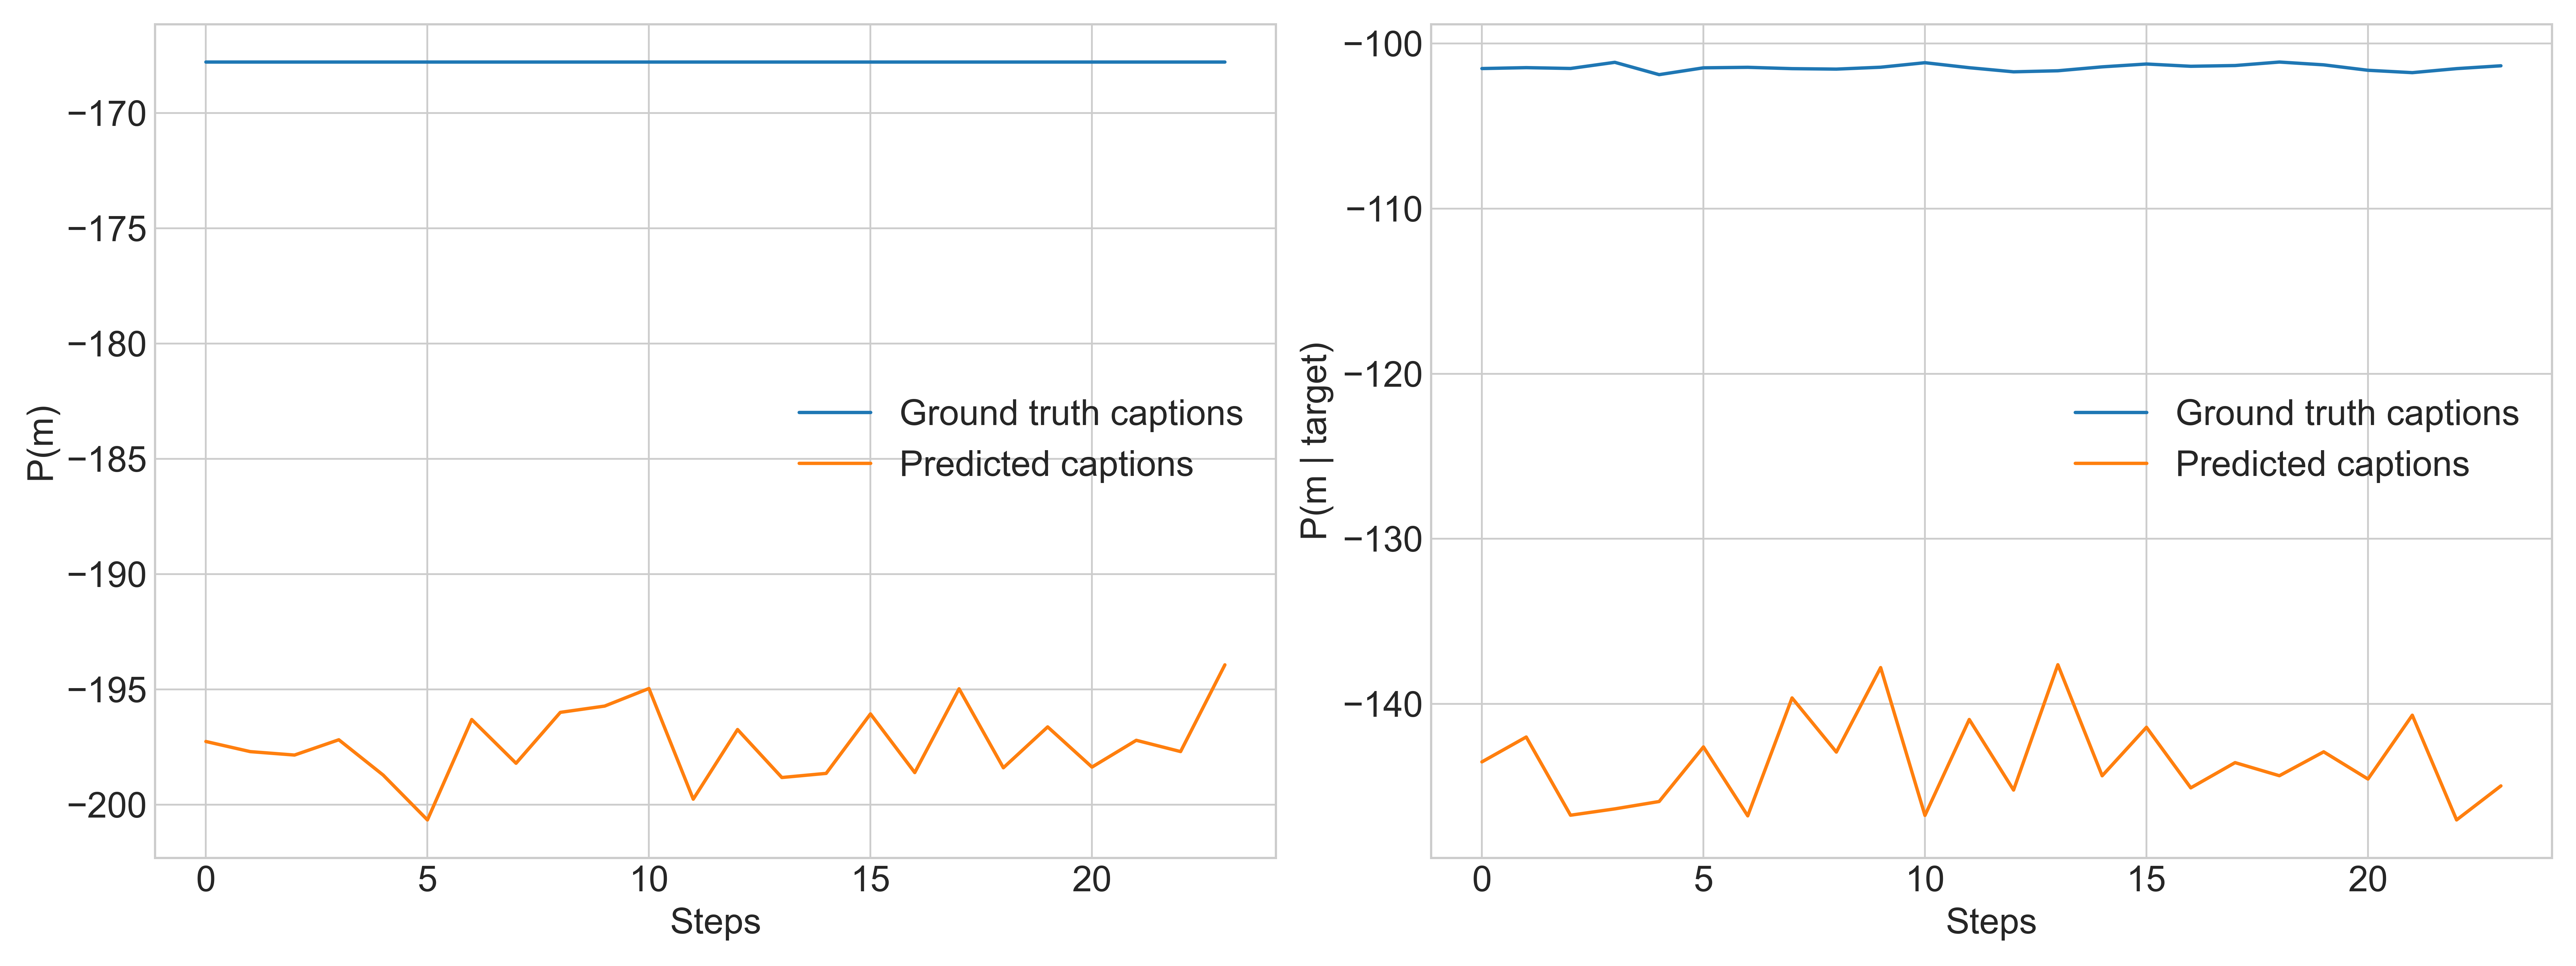
\includegraphics[width=\linewidth]{images/3dshapes_baseline_structural_semantic_drift_49_pure_075_similarFixed.png}
	\caption{Drift computed every 200 training steps on 192 images in the similar image pairs 3Dshapes experiment, with training image pairs matching with respect to fixed features (pure decoding, $L_s = 0.75$). The validation image pairs were constructed at random. Higher values are better. Left: Structural drift of ground truth and predicted captions. Right: Semantic drift of ground truth and predicted captions under the model pretrained on similar image pairs.} 
	\label{fig:3dshapes_similarFixed_075_str_sem_drift}
\end{figure}
\pt{Add results to table, finish discussion, compare convergence speed to randomly chosen similar pairs, overall random pairs experiment}


\subsection{3Dshapes: Fixed Listener Experiments}

Similarly to MS COCO in Section \ref{exp:coco_fixed_listener}, \textbf{H6} was also investigated for the 3Dshapes dataset in an analogous set up. The fixed listener was pretrained on exhaustive captions, and showed a post-pretraining test accuracy of 0.998 on ground truth test captions and 0.920 with the retrained speaker messages. 

The results on 3Dshapes patterned with those on MS COCO both in terms of training dynamics (Fig.~\ref{fig:3dshapes_fixed_listener_0_075_speaker_losses_listener_acc}) and the listener test accuracy being lower than for the joint listener experiment and the pretrained speaker (Tab.~\ref{tab:3dshapes_drift_metrics_basic}). The lower accuracy compared to the pretrained speaker could be attributed to the fact that the listener was pretrained on ground truth captions and then tested with speaker generated captions which are somewhat different from the ground truth due to the auto-regressive pretraining (see Appendix \ref{app:grid_search}), while the pretrained speaker was tested with the jointly trained listener from the baseline experiment.
\begin{figure}
	\centering
	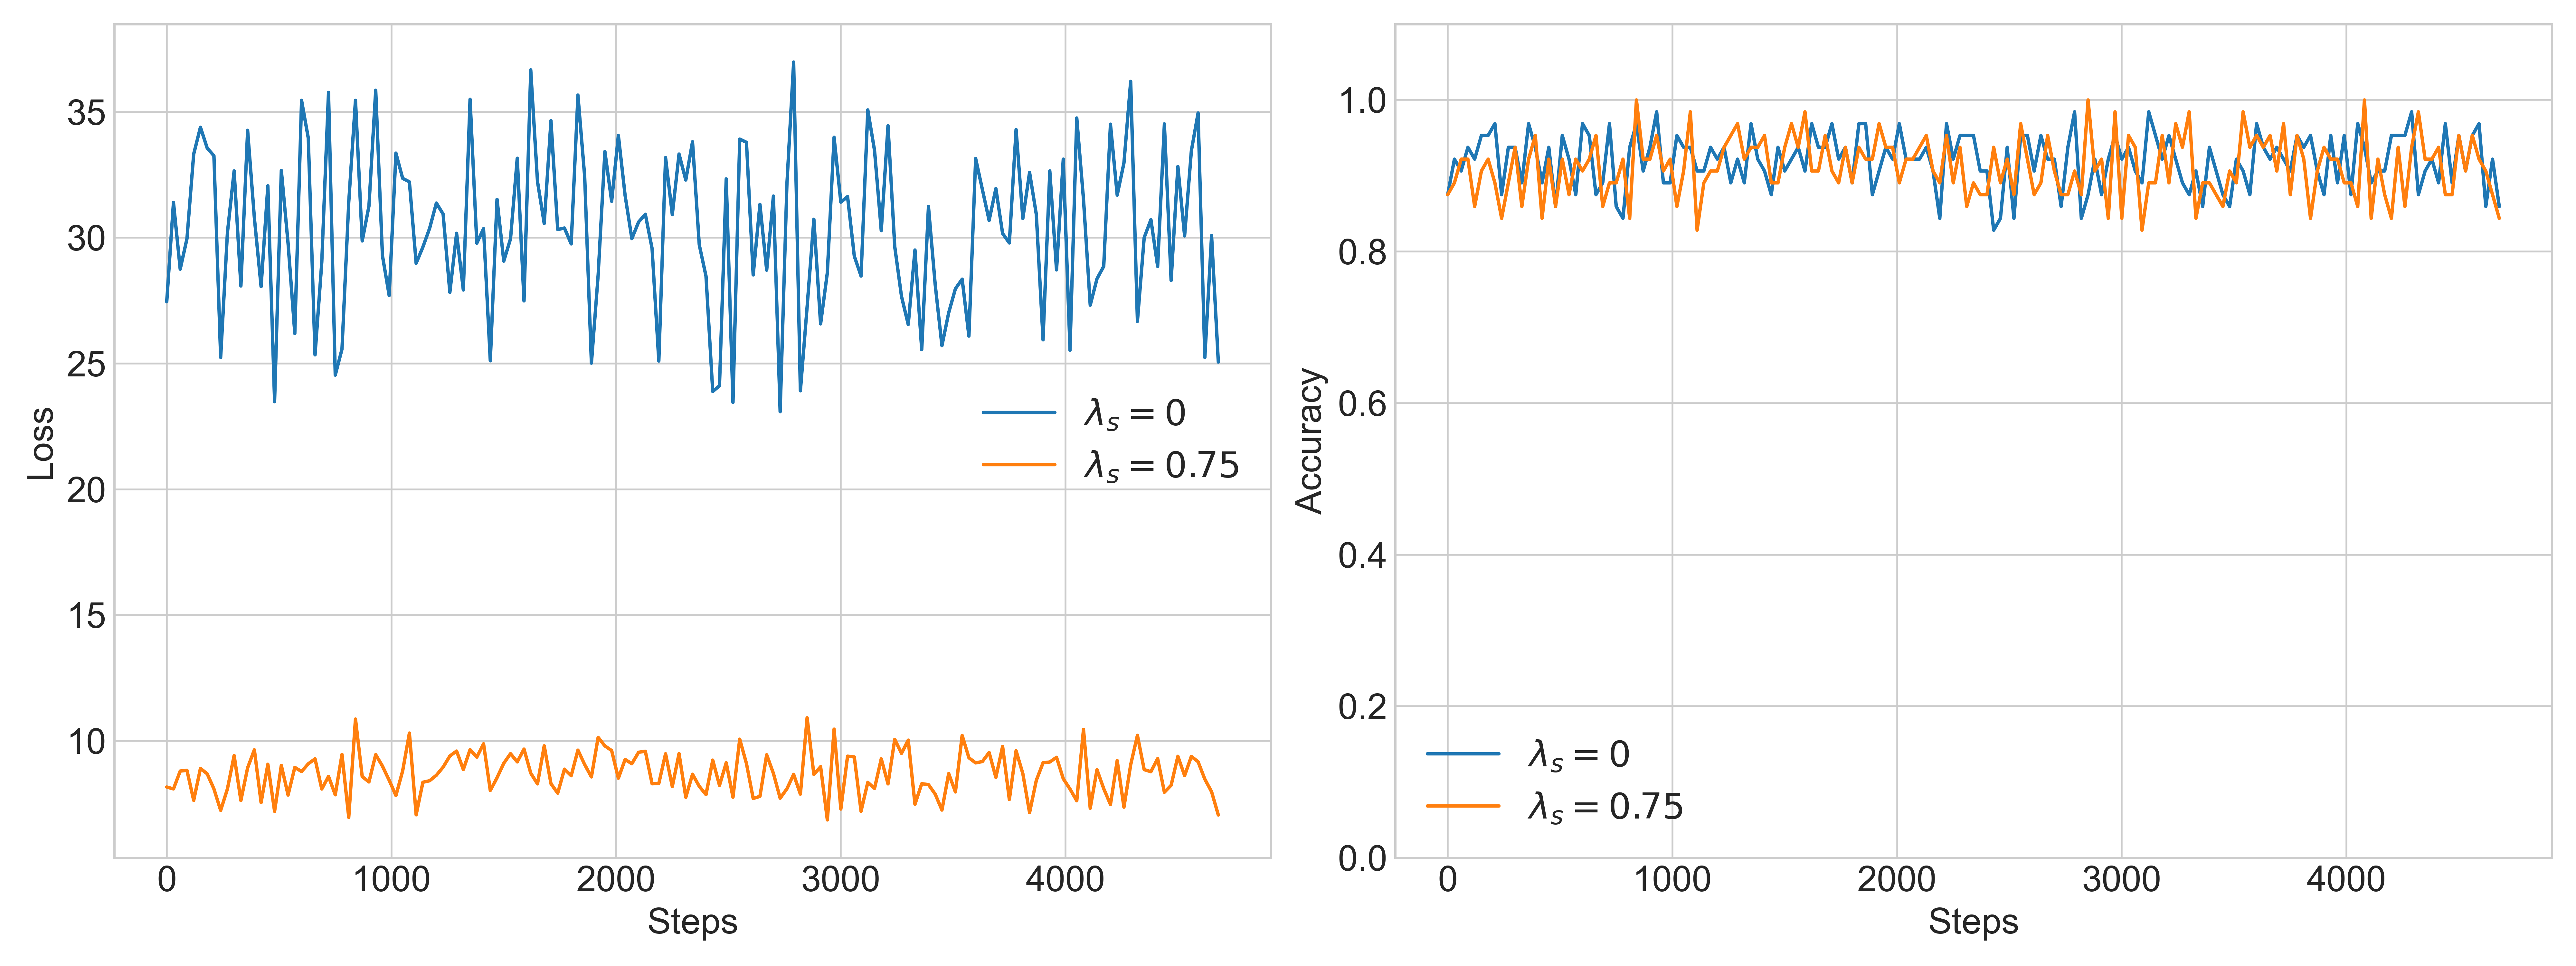
\includegraphics[width=\linewidth]{images/3dshapes_fixedListener_baseline_random_0_075_losses.png}
	\caption{Training results of reference games against a fixed listener on exhaustive captions of 3Dshapes (pure decoding, $\lambda_s=0$ vs. $\lambda_s=0.75$). Left: Total speaker training loss. Right: Listener training accuracy.}
	\label{fig:3dshapes_fixed_listener_0_075_speaker_losses_listener_acc}
\end{figure}

Similarly to MS COCO, training the speaker against a fixed listener also mitigated both structural and semantic drift (Tab.~\ref{tab:3dshapes_drift_metrics_basic}). In fact, the drift decreased even compared to the pretrained speaker. This suggests that in a smaller action space of the 3Dshapes experiment, the functional training signal from the listener pretrained on ground truth captions might be strong enough to further fine-tune the speaker towards more ground truth-like messages. The intuition that this signal seems to rather pressure the speaker towards ground truth like captions than towards strong functional improvement is supported by an absense of definitve increases in the overlap metrics, compared to the pretrained speaker (Tab. \ref{tab:3dshapes_drift_metrics_basic}). 
\pt{TODO image caption evaluation}
\begin{figure}
	\centering
	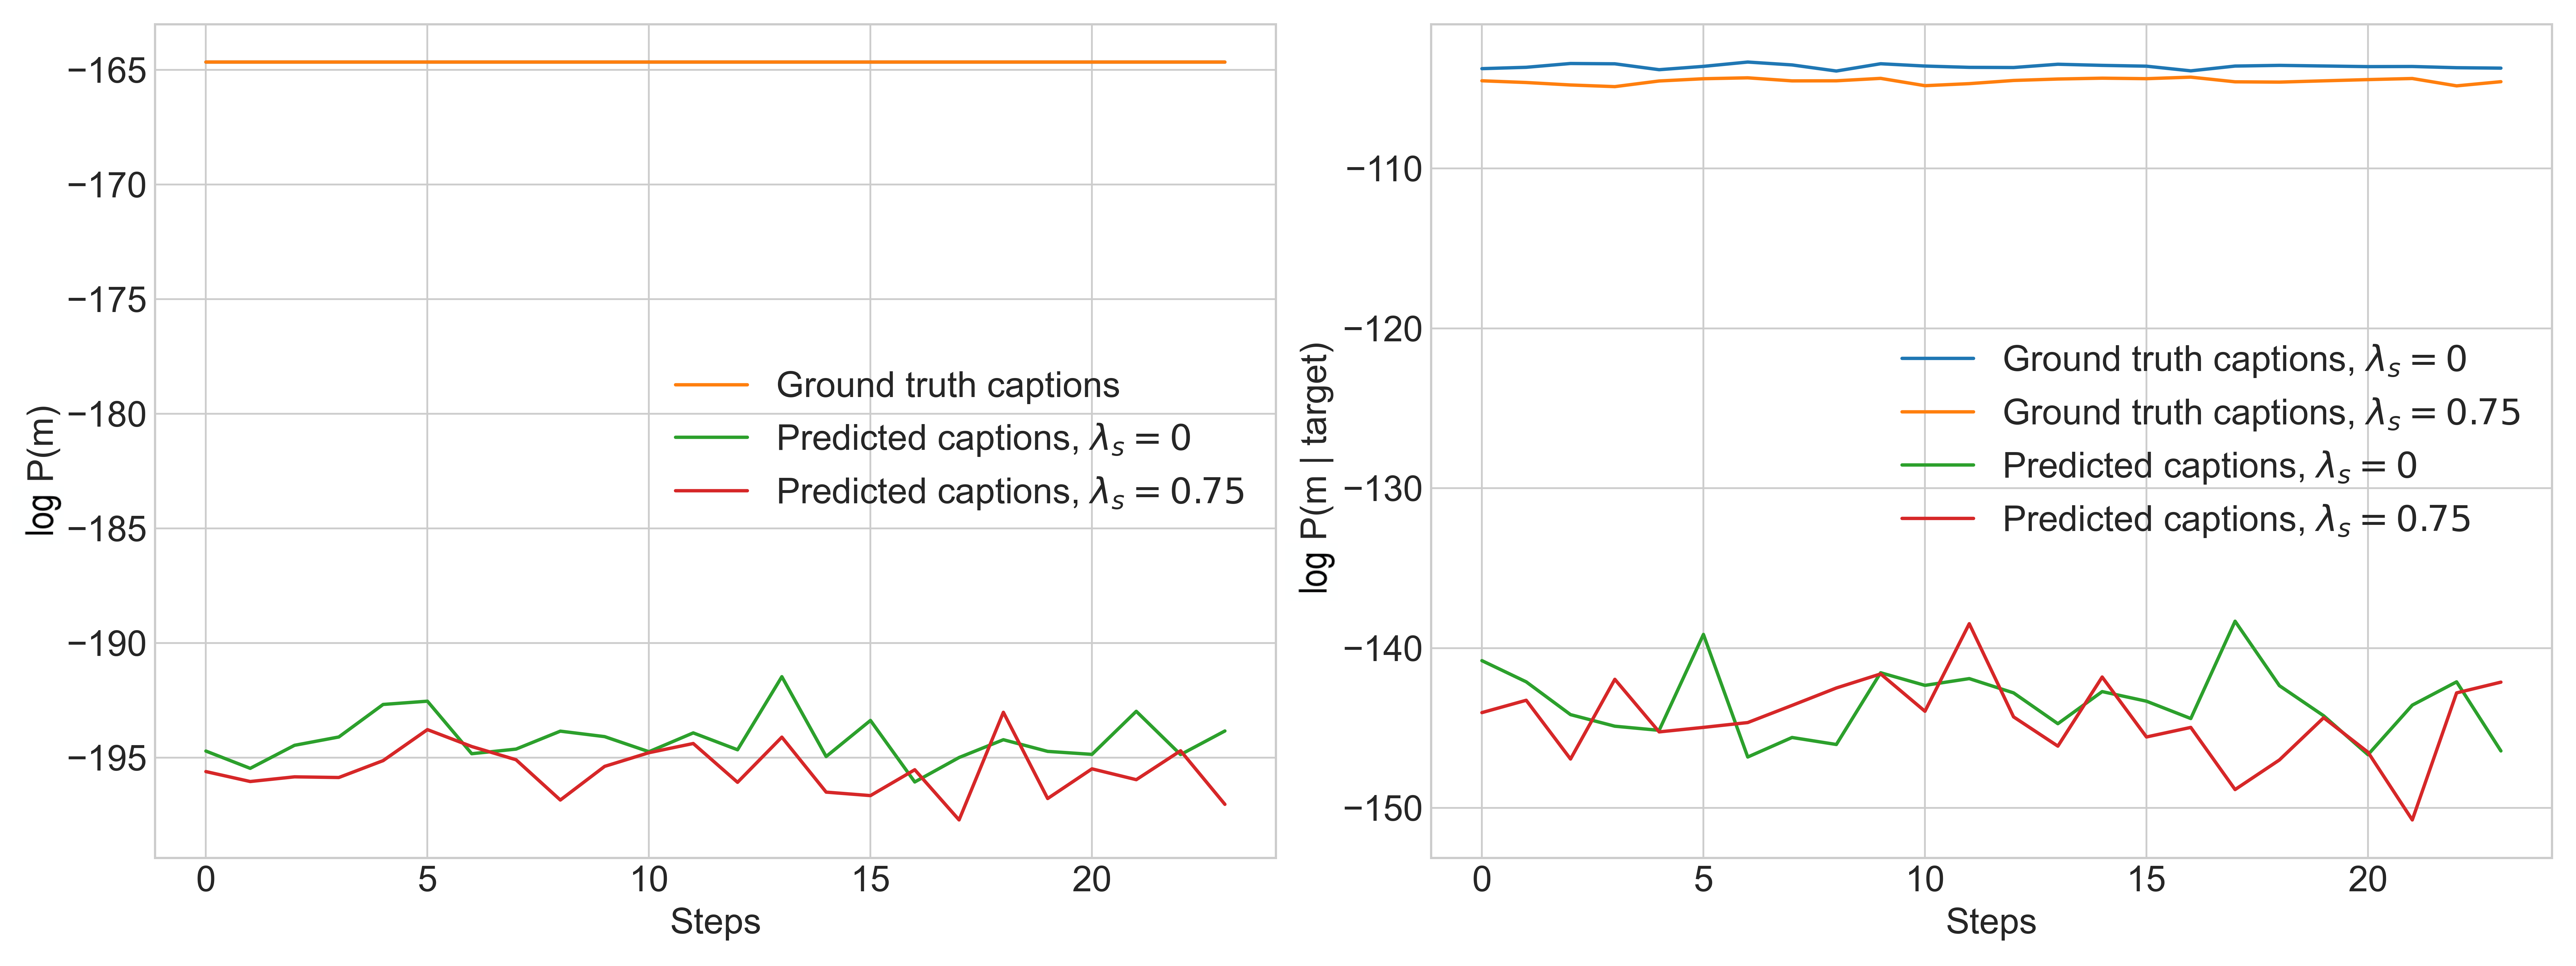
\includegraphics[width=\linewidth]{images/3dshapes_fixedListener_structural_semantic_drift_49_pure_0_075_random.png}
	\caption{Drift dynamics computed during reference game training with the fixed listener on 3Dshapes (pure decoding, $\lambda_s=0$ vs. $\lambda_s=0.75$). Higher values indicate less drift. Left: Structural drift of ground truth and predicted captions under the pretrained Transformer XL model. Right: Semantic drift of ground truth and predicted captions under the pretrained speaker model.}
	\label{fig:3dshapes_fixed_listener_0_075_str_sem_drift}
\end{figure}

In order to investigate whether it is indeed the functional task signal that is responsible for mitigating the language drift, a follow-up experiment with a functional loss only (i.e., $\lambda_s=0$) was also conducted for 3Dshapes. While the task success was not visibly improved (see Fig.~\ref{fig:3dshapes_fixed_listener_0_075_speaker_losses_listener_acc}, right, orange vs. blue line), structural and semantic drifts during training were indeed slightly lower for $\lambda_s=0$, compared to $\lambda_s=0.75$ (Fig.~\ref{3dshapes_fixed_listener_0_075_str_sem_drift}, green line being slightly above the red one).\footnote{Semantic drift values of the ground truth are slightly different due to the known non-deterministic behaviour of some CUDA supporting RNN implementations in Pytorch, even with a random seed.} Validation results in Table \ref{tab:3dshapes_drift_metrics_basic} indicate that semantic drift was better mitigated under a stronger functional training signal ($\lambda_s =0$ compared to $\lambda_s =0.75$), suggesting that the grounding was better preserved. Structural drift, however, increased, compared to $\lambda_s =0.75$, which is expected given that there was no structural learning signal anymore in the $\lambda_s =0$ experiment. Further confirming intuitions regarding the role of the functional learning signal, the discrete overlap increased in the $\lambda_s =0$ configuration, outperforming the baseline joint listener experiment. The continuous overlap, on the other hand, decreased, compared to both pretrained and baseline joint speakers, indicating that the functional improvements might not be translated to topographic effects in the embedding space. \pt{cheeeeeck this attempt to be fancy. or at least circle to topographic mesaures by e g \cite{lazaridou2020emergent}} 

To sum up, \textbf{H6} is also supported by the data in the 3Dshapes experiment. Similarly to MS COCO, one can infer that reference game performance is at least partly carried by speaker-listener co-adaptation, and that the functional signal available from the pretrained listener might rather have structural effects in this smaller action space, than lead to functional improvement. \pt{double check}  

\subsection{3DShapes: Short Captions Experiment}
\label{expt:3dshapes_short}

\begin{table}[] 
	\begin{tabularx}{\textwidth}{|X|l|l|X|X|X|X|}
		\hline
		\textbf{Model name}                                    & \textbf{log $P(m)$} & \textbf{log $P(m \mid i)$} & \textbf{Overlap (d)} & \textbf{Overlap (c)} & \textbf{Listener acc (random)} & \textbf{Listener acc (similar)} \\ \hline
		Ground truth mixed       &     -139.026            &    -80.323             &       7.401        &        0.028        &                 &                \\ \hline
		Pretrained 3D mixed speaker    &      -192.903           &         -59.623               &        2.309              &      -0.001                & 0.944 (baseline listeners)                 &                 \\ \hline
		3D Baseline, random  &       -195.495        &           -147.313           &          5.247            &         0.001             & 0.979                                    &                        0.959                   \\ \hline
		%3D Baseline, similar all, $\lambda_s = 0.75$ &      -198.189             &       -140.786                 &           5.578           &        0.001              & 0.878                      &            0.906                        \\ \hline
		3D Baseline, similar fixed, random test &       -193.709            &    -141.010                  &        3.280            &      -0.003         &            0.688       &                           \\ \hline
		3D Baseline, similar fixed, same test &      -199.014        &        -146.280           &        2.875       &      0.029   &              &          0.691                   \\ \hline
		3D Baseline, similar fixed, diff. test &       -197.539        &       -146.362           &   2.705          & 0.030    &                &              0.561     / 0.705           \\ \hline
		3D Short, random&      -189.285             &      -58.278                  &             2.316        &         0.000             &                   0.957                       &                                           \\ \hline
		%3D Short, similar all, $\lambda_s = 0.75$&      -145.014             &      -76.474                  &             1.565         &         0.000             &                   0.885                       &                                           \\ \hline
		3D Short, similar fixed, random test&      -188.249           &     -121.830                  &             1.839         &         -0.001             &                   0.726                       &                                        \\ \hline
		3D Short, similar fixed, same test&      -192.130      &     -58.753      &   0.837      & 0.003      &                       &               0.723                           \\ \hline
		3D Short, similar fixed, diff. test &  -189.320       & -58.463     & 1.663        &  0.003         &      &     0.562 / 0.751         \\ \hline
	\end{tabularx}
	\caption{\label{tab:3dshapes_drift_metrics_basic_short} Language drift metrics and listener test accuracies of similar pairs experiments on the 3Dshapes dataset. 
		``Baseline'' refers to the setup wherein the listener is trained jointly with the speaker, using pure decoding, using exhaustive captions only. ``Random'' refers to speakers trained on random target-distractor pairs; ``similar'' refers to speakers trained on similar target-distractor pairs. $\lambda_s = 0.75$ is used in all experiments.}
\end{table}

The goal of this experiment is to address \textbf{H10} by conducting experiments wherein the speaker produced captions of varying granularity.
To this end, the second speaker pretrained on mixed-length captions was used (see Section \ref{speaker_pretraining}). During reference game training, the structural loss was also computed against ground truth captions of varying length. That is, the targets that the speaker had to refer to during training were associated with both exhaustive and short ground truth captions. Otherwise, the training procedure was identical to previous experiments.

These experiments addressed several aspects. First, they addressed the question whether the presence of exhaustive captions (as was the case in the baseline experiment) was necessary for successful task completion. Second, they addressed whether absense of exhaustivity might be the reason for language drift because the speaker might have to resort to drift strategies in order to complete the functional task due to a lack of linguistic task-appropriate resources. 
Third, speaker flexibility to generate messages of variable length in absense of explicit message length regularization was investigated. 

\begin{figure}
	\centering
	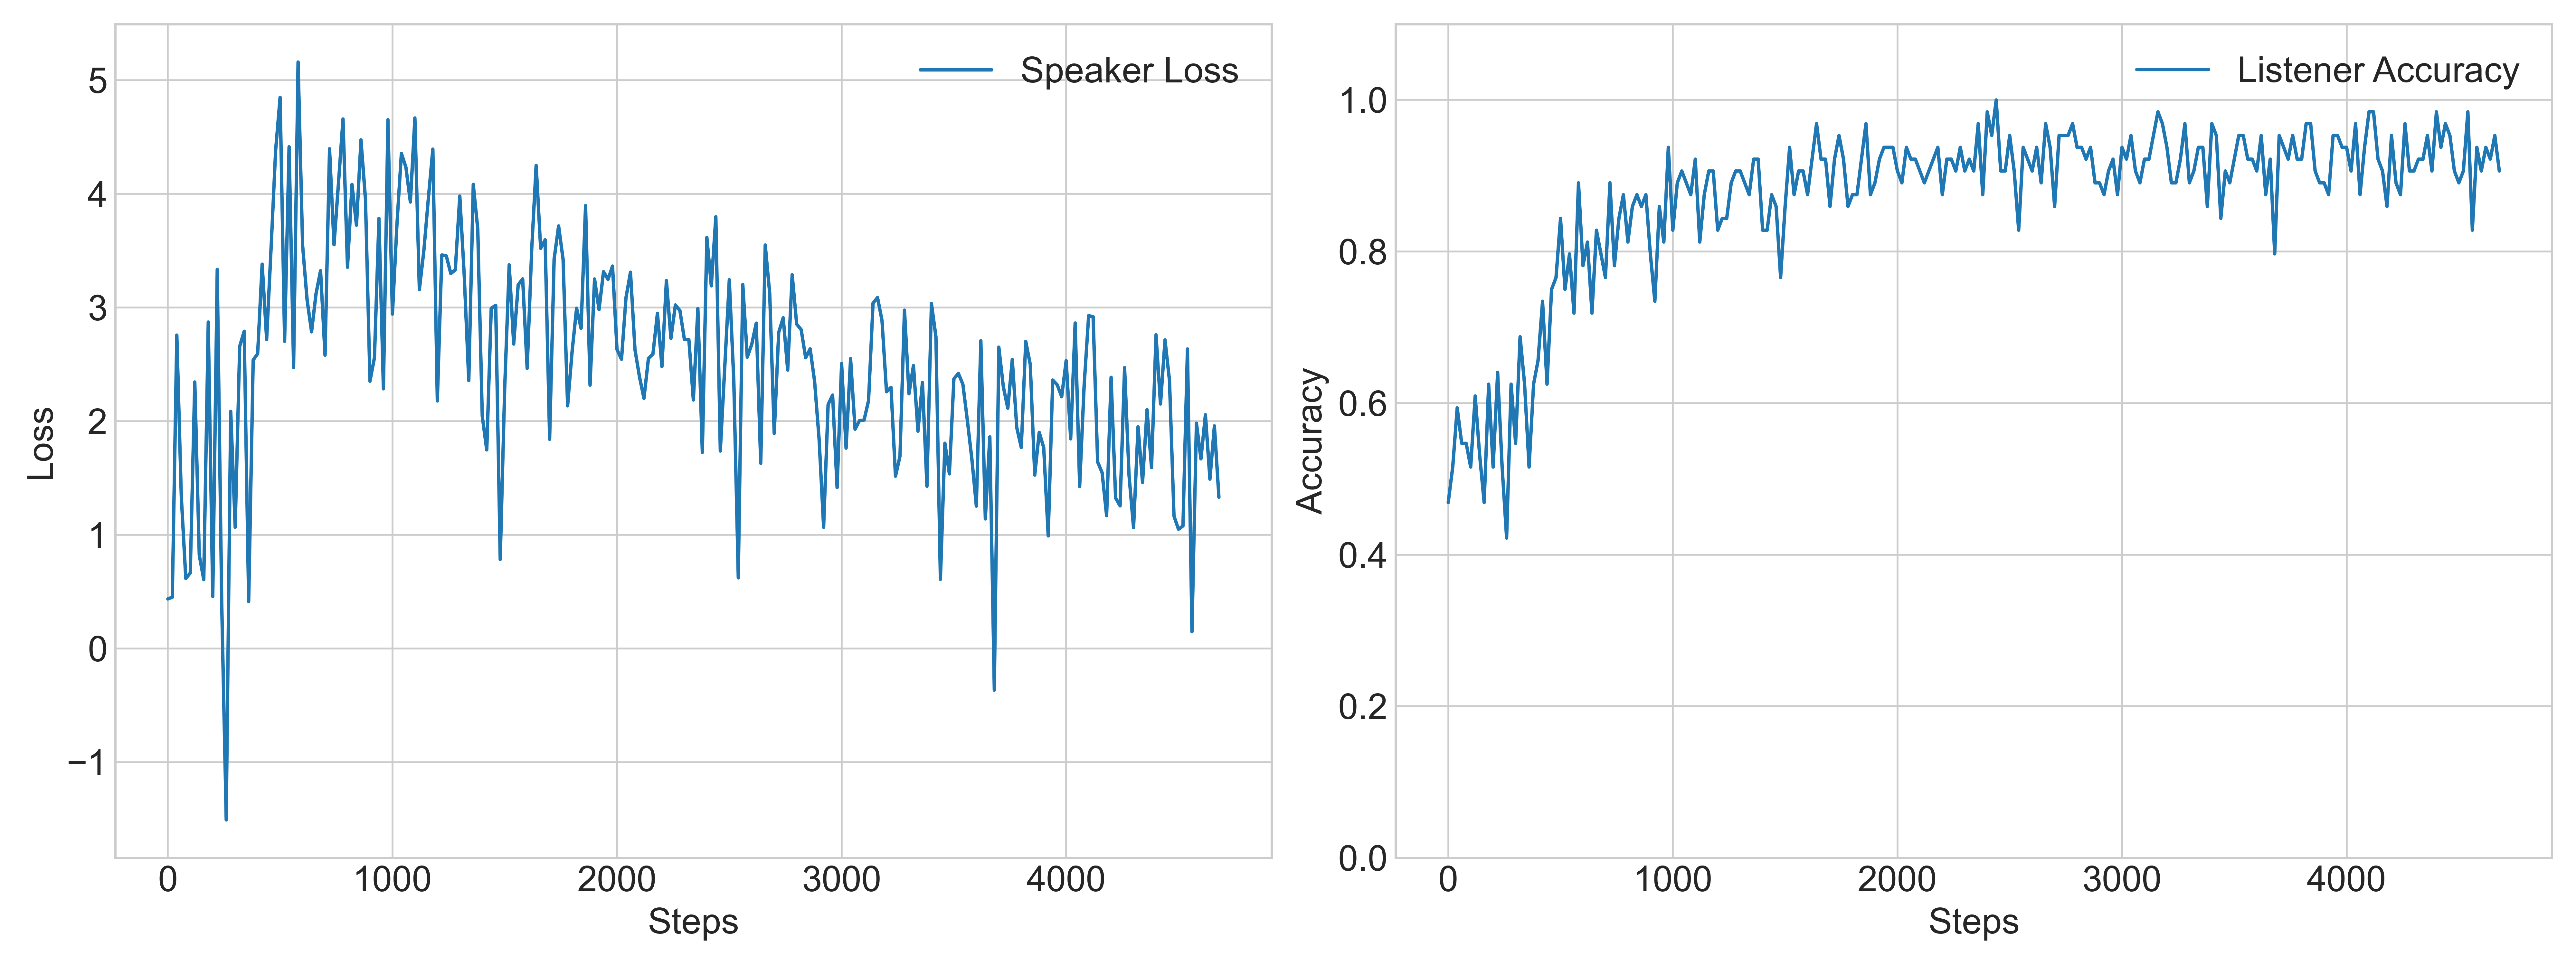
\includegraphics[width=\linewidth]{images/3dshapes_wShort_baseline_random_075_losses.png}
	\caption{Training results of the baseline reference game on both short and exhaustive captions of 3Dshapes (pure decoding, $\lambda_s=0.75$). Left: Total speaker training loss. Right: Listener training accuracy.}
	\label{fig:3dshapes_wShort_075_speaker_losses_listener_acc}
\end{figure}

First, the baseline experiment with pure decoding and $\lambda_s = 0.75$ with the mixed captions was conducted. Similar to the testing procedure in previous experiments, the model was evaluated in terms of listener accuracy and language drift on the same 1000 held out images. For the test set, it was now also chosen at random whether a target image was associated with three short or exhaustive ground truth captions out of five, in order to compute drift metrics of the ground truth captions. Therefore, the drift measures of the ground truth differ from the exhaustive ground truth captions.
The training results can be seen in Figure~\ref{3dshapes_wShort_075_speaker_losses_listener_acc}. Based on visual comparison to the exhaustive captions baseline experiment (Fig.~\ref{fig:3dshapes_baseline_075_speaker_loss_listener_acc}), no qualitative differences in either speaker convergence or listener training performance could be observed. Nontheless, listener test accuracy decreased by 0.022 compared to exhaustive baseline (Tab.~\ref{tab:3dshapes_drift_metrics_basic}).
This rather small difference could be because in this experiment the target and distractor images were paired at random and were, therefore, likely quite dissimilar, intuitively rendering the presence of exhaustive messages not necessary for successful reference.

Turning towards language drift, one can observe that both structural and semantic drift during training were lower for this experiment compared to the exhaustive experiment (Fig.~\ref{fig:3dshapes_wShort_075_str_sem_drift} vs. Fig.~\ref{fig:3dshapes_baseline_075_str_drift}), showing an opposite to the hypothesized effect. The lower structural drift could be attributed to generally higher naturalness of the short captions compared to the exhaustive ones, thus, rendering them more likely under a pretrained language model. The lower semantic drift which additionally was lower for the generated captions than for the ground truth ones might indicate that the speaker was further fine-tuned to produce messages that were more similar to the ground truth. This might be easier than for exhaustive captions because of the shorter effective message length which is advantageous for RNN training \parencite[cf.][]{jaeger2002tutorial}. This is further cofirmed by the validation drift results. Structural drift was lower compared to both the exhaustive baseline and the pretrained speaker. However, the absolute difference to the drift value of the ground truth captions is much larger for mixed captions (50.259) compared to the exhaustive experiment (30.743) (Tab.~\ref{tab:3dshapes_drift_metrics_basic}). This might suggest that due to the varying length of messages and the respective variation in sentence structure the speaker might struggle more to produce syntactically well-formed sentences after fine-tuning. 
Similarly, semantic drift was lower for mixed captions compared to the both exhaustive and pretrained speakers. The absolute difference in semantic drift of the fine-tuned speaker and the ground truth captions was 22.045 for mixed captions and 39.457 for the exhaustive experiment, where in the former the speaker actually improved over ground truth captions, while the latter was worse (Tab.~\ref{tab:3dshapes_drift_metrics_basic}). This might indicate that further supervised fine-tuning of the speaker model took place for the mixed but not the exhaustive captions. Again, this could be attributed to the effective message length difference of the ground truth captions and the respective difficulty of training.
Regarding overlap metrics, the discrete overlap decreased much more drastically compared to ground truth for the mixed captions than for exhaustive ones. This low value might be confounded with the variation of the granulaity of a sampled ground truth caption, and not be directly representative of functional performance. For instance, during evaluation, the speaker might have generated a valid discriminative short caption, but the sampled corresponding ground truth was an exhaustive caption, yielding a low overlap value.   
\pt{Also add a line for the pretrianed short captions speaker in the drift table, and actually compare to that. }

\begin{figure}
	\centering
	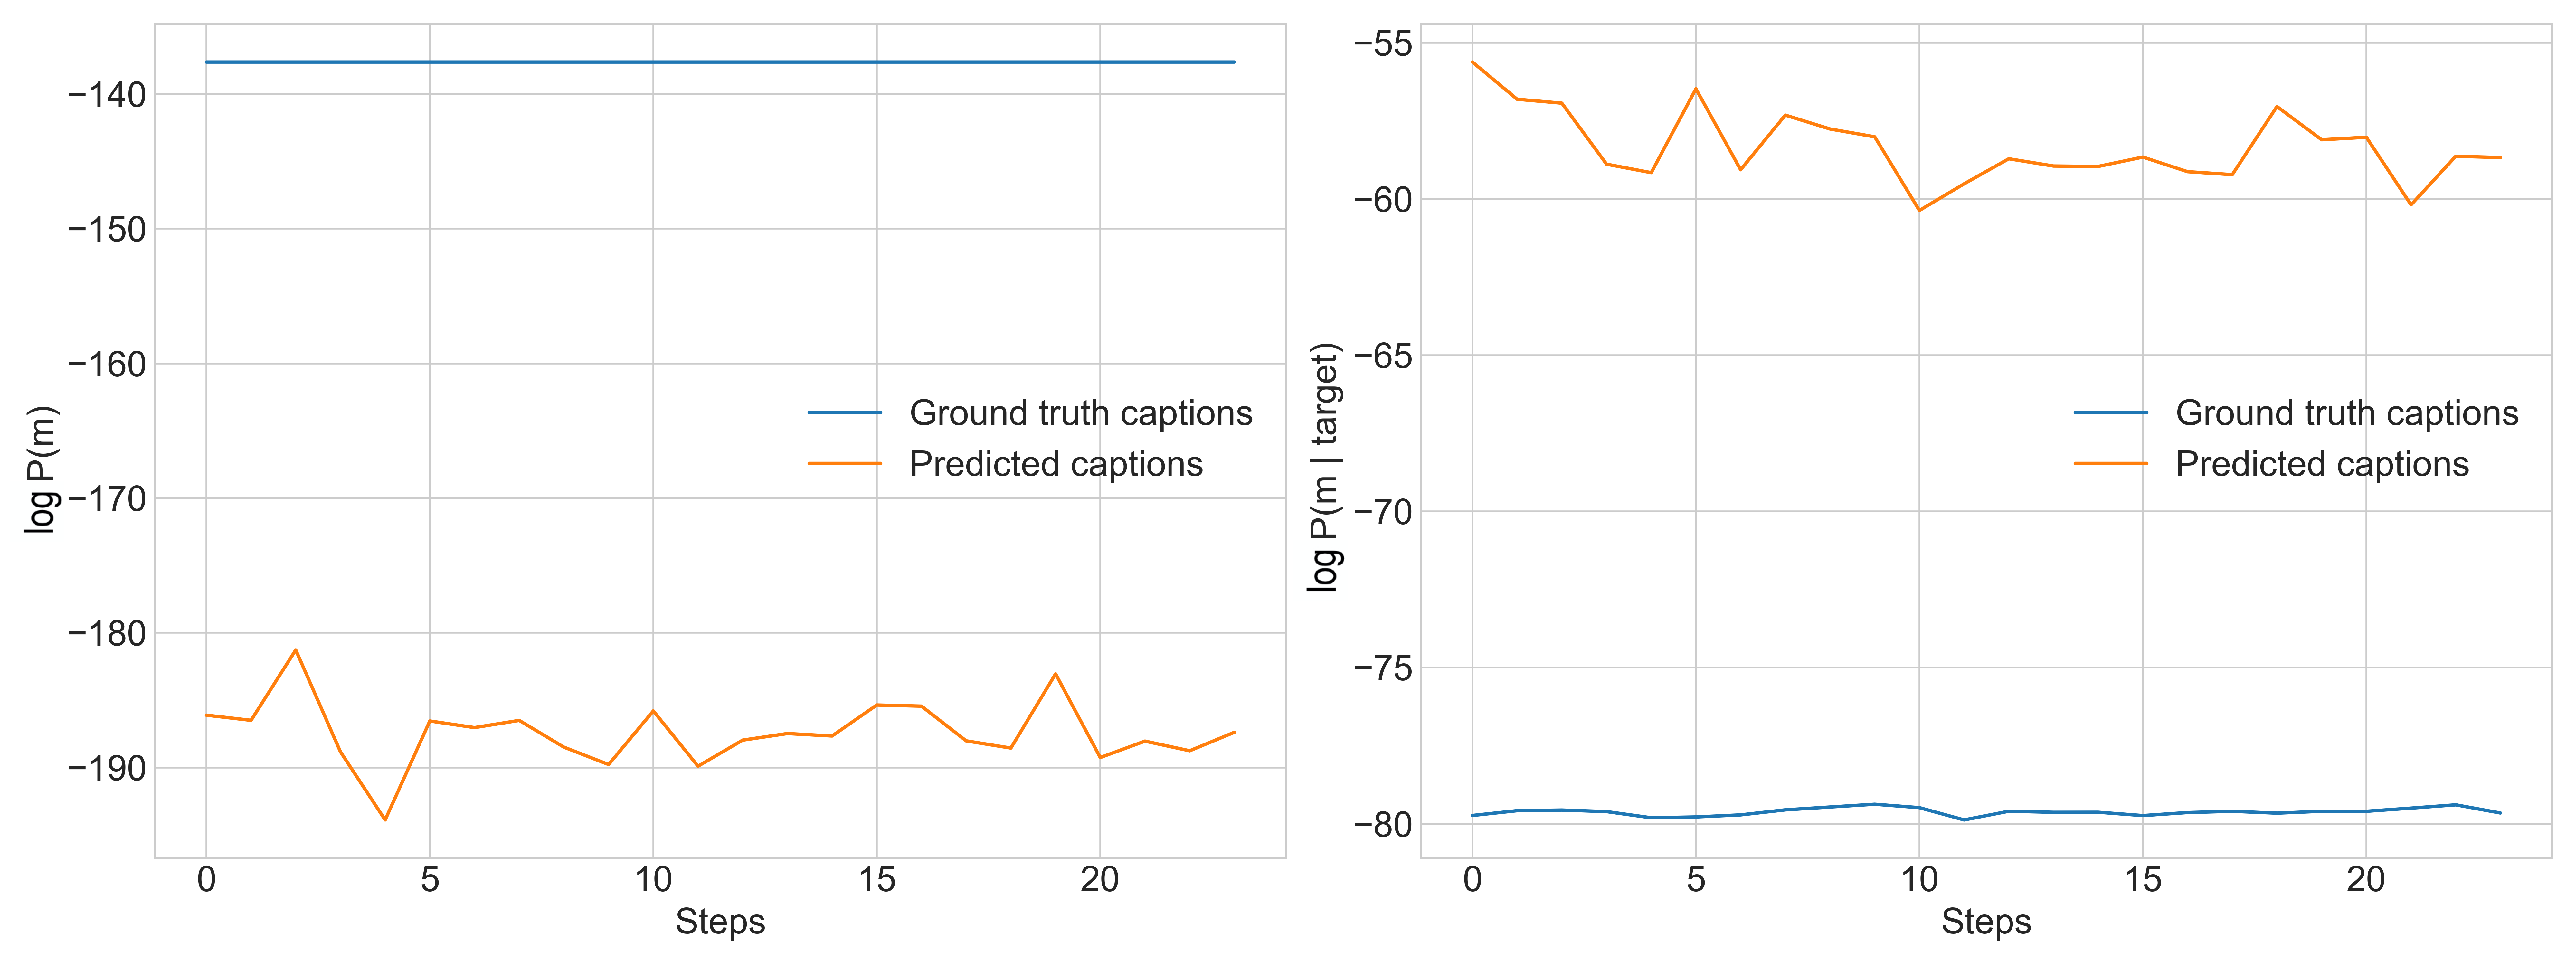
\includegraphics[width=\linewidth]{images/3dshapes_wShort_structural_semantic_drift_49_pure_075_random.png}
	\caption{Drift dynamics computed during reference game training on both short and exhaustive captions of 3Dshapes (pure decoding, $\lambda_s=0.75$). Higher values indicate less drift. Left: Structural drift of ground truth and predicted captions under the pretrained Transformer XL model. Right: Semantic drift of ground truth and predicted captions under the pretrained speaker model.}
	\label{fig:3dshapes_wShort_075_str_sem_drift}
\end{figure}

%\pt{!!! Normalization of the drift measures by average length in order to make exhaustive and short caps comparable!!!}
In order to investigate the third aspect---speaker's generation length flexibility---lengths of the captions generated by the speaker on the validation set were computed. These were calculated by counting the number of tokens until the first occurrence of the special END token in the message (excluding them). As can be seen in Figure~\ref{fig:3dshapes_exh_short_random_lengths}, the speaker that saw short captions during pretraining and in the reference game has learned to produce captions with varying length with approximately uniform probability, except for a bias towards generating captions of maximal allowed length  around one third of the time. This bias can also be observed for the exhaustive captions only speaker, whose generated caption lengths matched the ones from the exhaustive training set. THese results hint at the importance of the training data distribution for the speaker's potential to adjust their message length, possibly responding to different granularity needs (see Section \ref{expt:3d_similar} for details). 

\begin{figure}
	\centering
	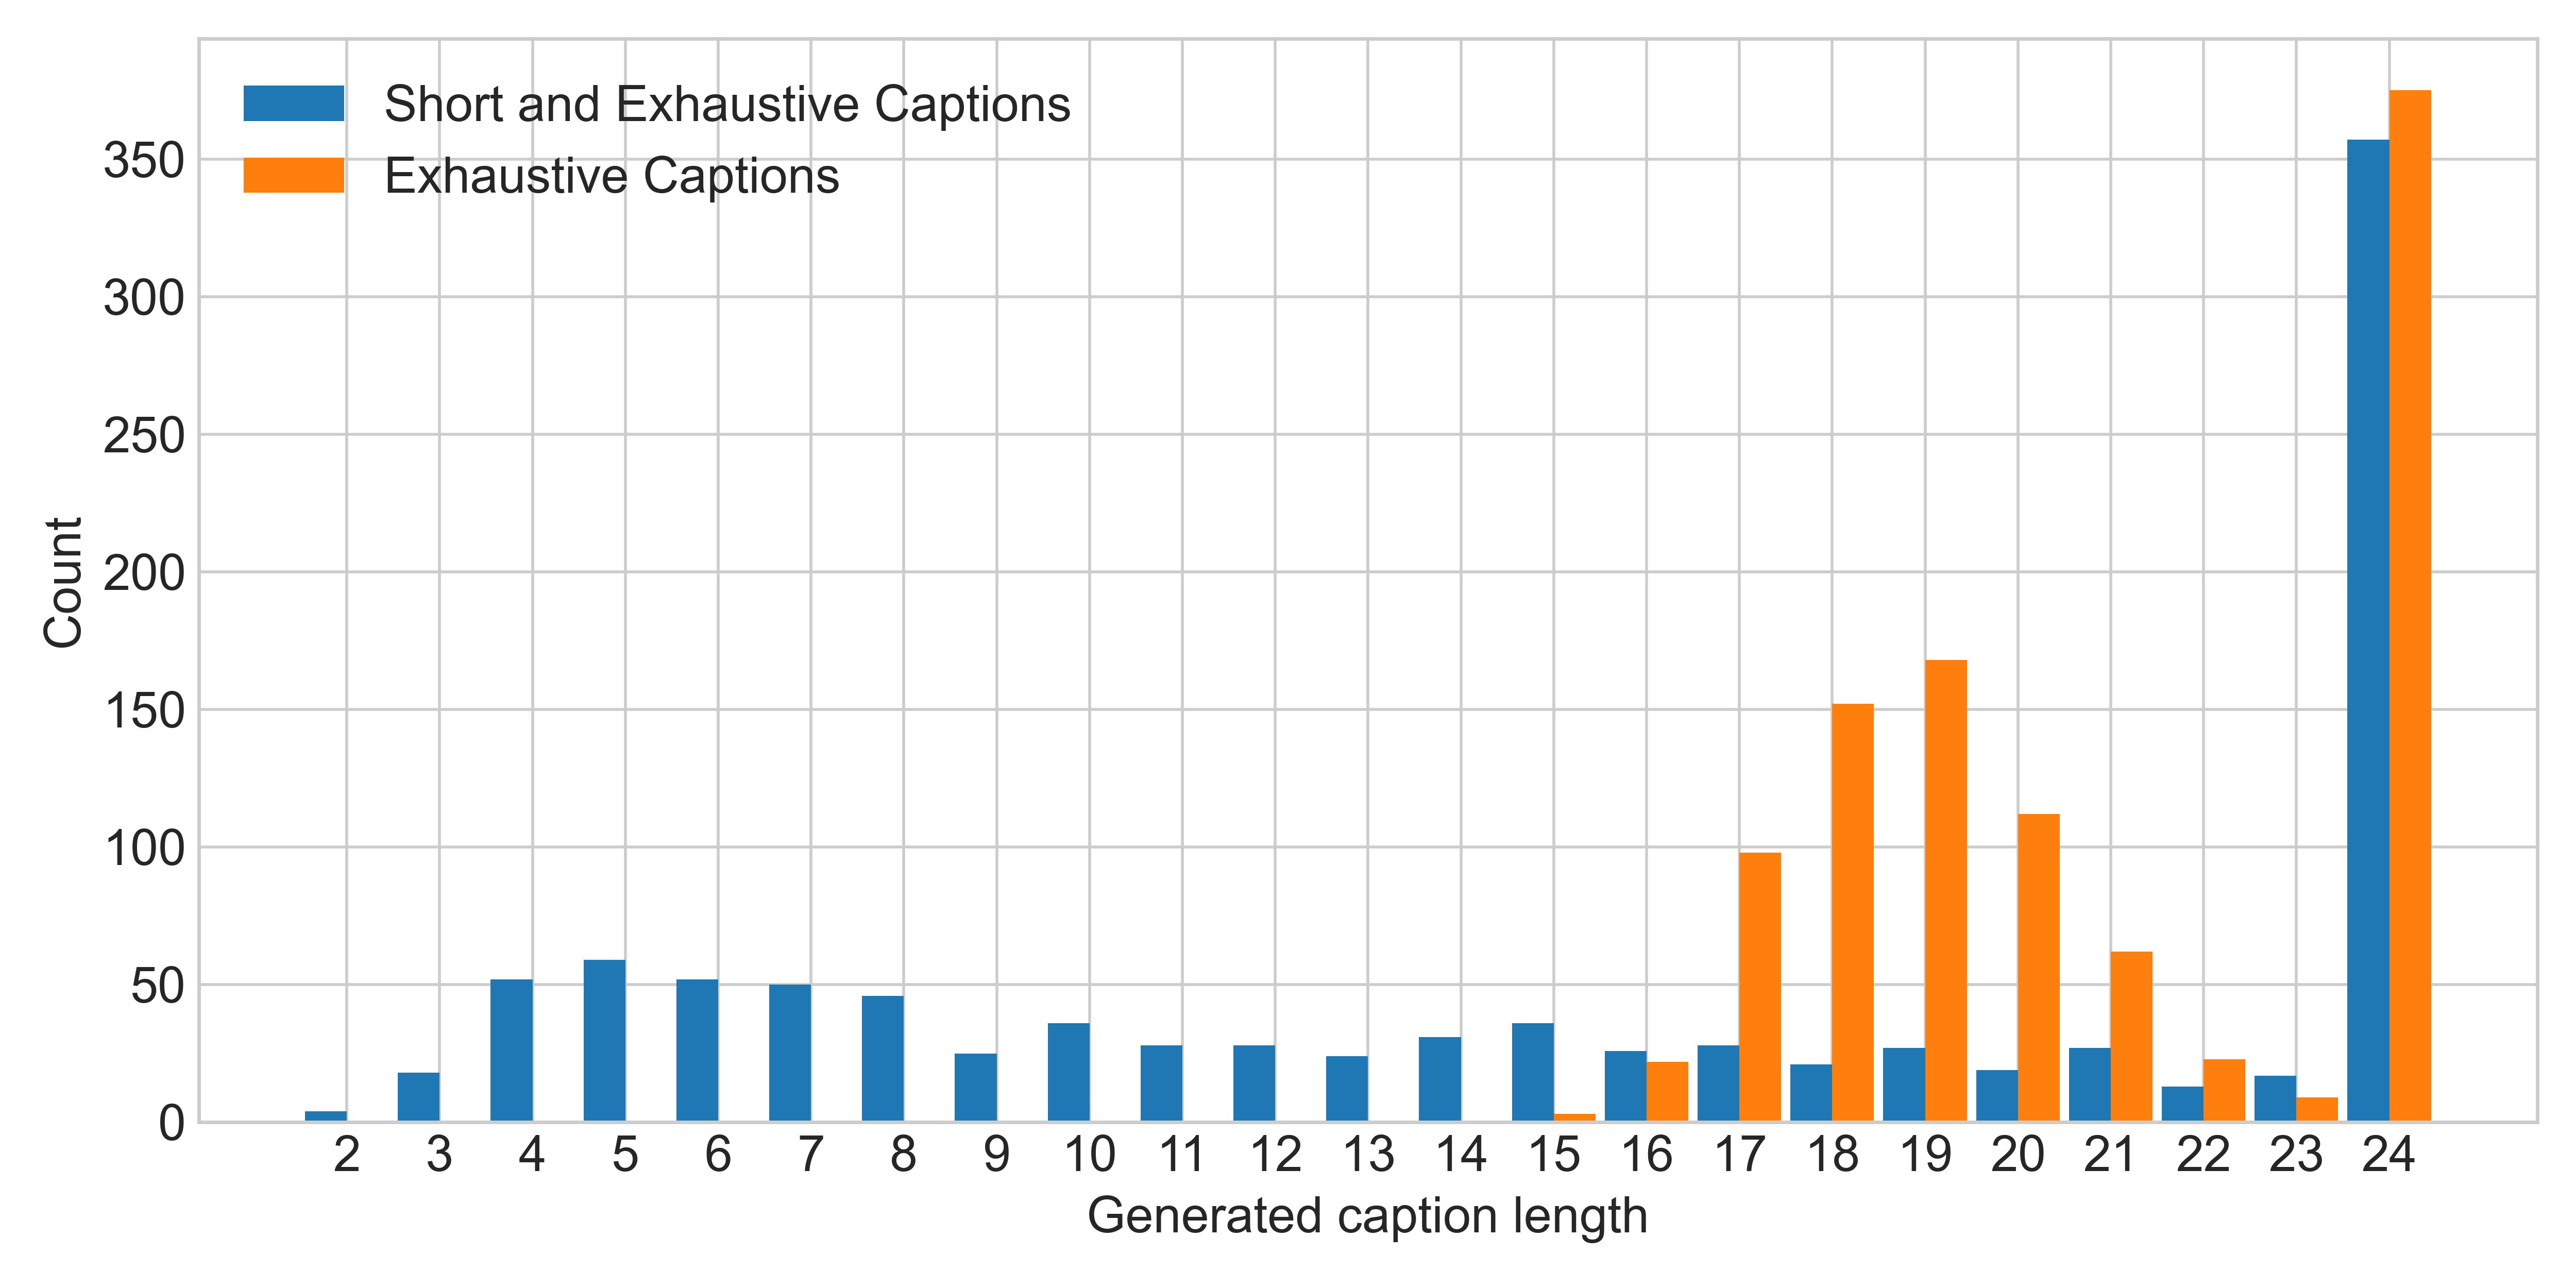
\includegraphics[width=0.7\linewidth]{images/3dshapes_exh_short_random_length_counts.png}
	\caption{Counts of effective sentence lengths generated on the validation dataset by the speakers from the exhaustive and the mixed-length experiments.}
	\label{fig:3dshapes_exh_short_random_lengths}
\end{figure}

In sum, \textbf{H10} is not supported by experimental results on random target-distractor pairs. In fact, language drift is even smaller compared to the exhaustive captions experiment. This suggests that architectural aspects like the length of messages the speaker is trained to generate have a larger influence on message quality than guaranteed presence of fully descriptive captions in the training dataset. At the same time, these results showed that the speaker is capable of flexibly varying her message length, if the respective inductive bias was provided during training. 

\subsubsection{Similar Pairs Experiment}
\label{expt:3d_similar}

In order to increase the pressure towards necessity of exhaustive descriptions, an experiment including short captions was conducted on \emph{similar} target-distractor image pairs. Again, the similar pairs were constructed such that the target and the distractor matched with respect to object shape, object color and background color. The effect of adding short captions during training compared to using exhaustive captions only can be seen in Figure~\ref{3dshapes_wShort_similarFixed_075_speaker_losses_listener_acc}. \pt{reference or remove old figure}.

\begin{figure}
	\centering
	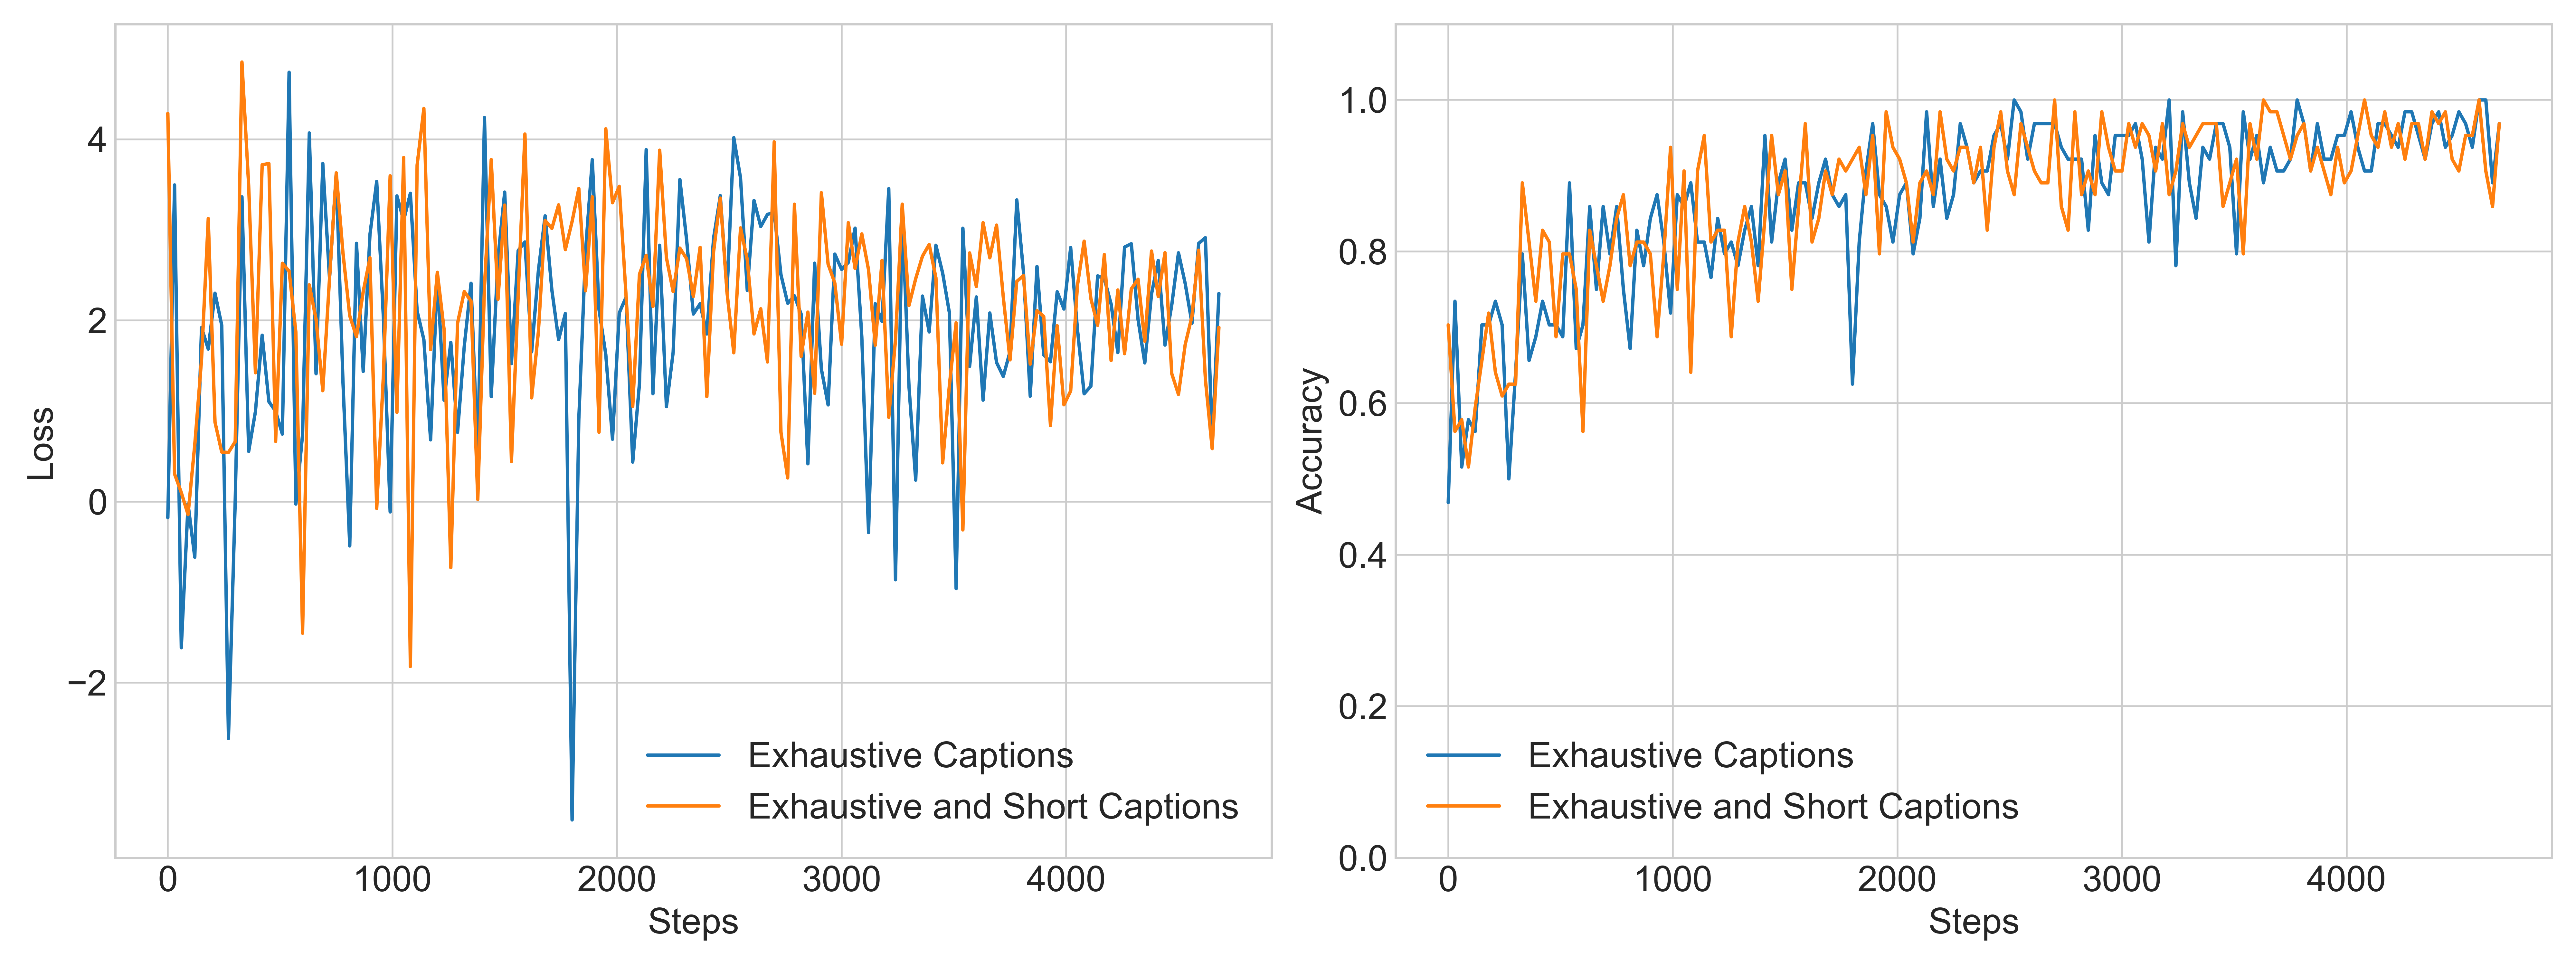
\includegraphics[width=\linewidth]{images/3dshapes_similarFixed_short_vs_exh_075_losses.png}
	\caption{Training results of the baseline reference game on both short and exhaustive captions of 3Dshapes on similar image pairs. Similar features were fixed (pure decoding, $\lambda_s=0.75$). Left: Total speaker training loss. Right: Listener training accuracy.}
	\label{fig:3dshapes_wShort_similarFixed_075_speaker_losses_listener_acc}
\end{figure}

\begin{figure}
	\centering
	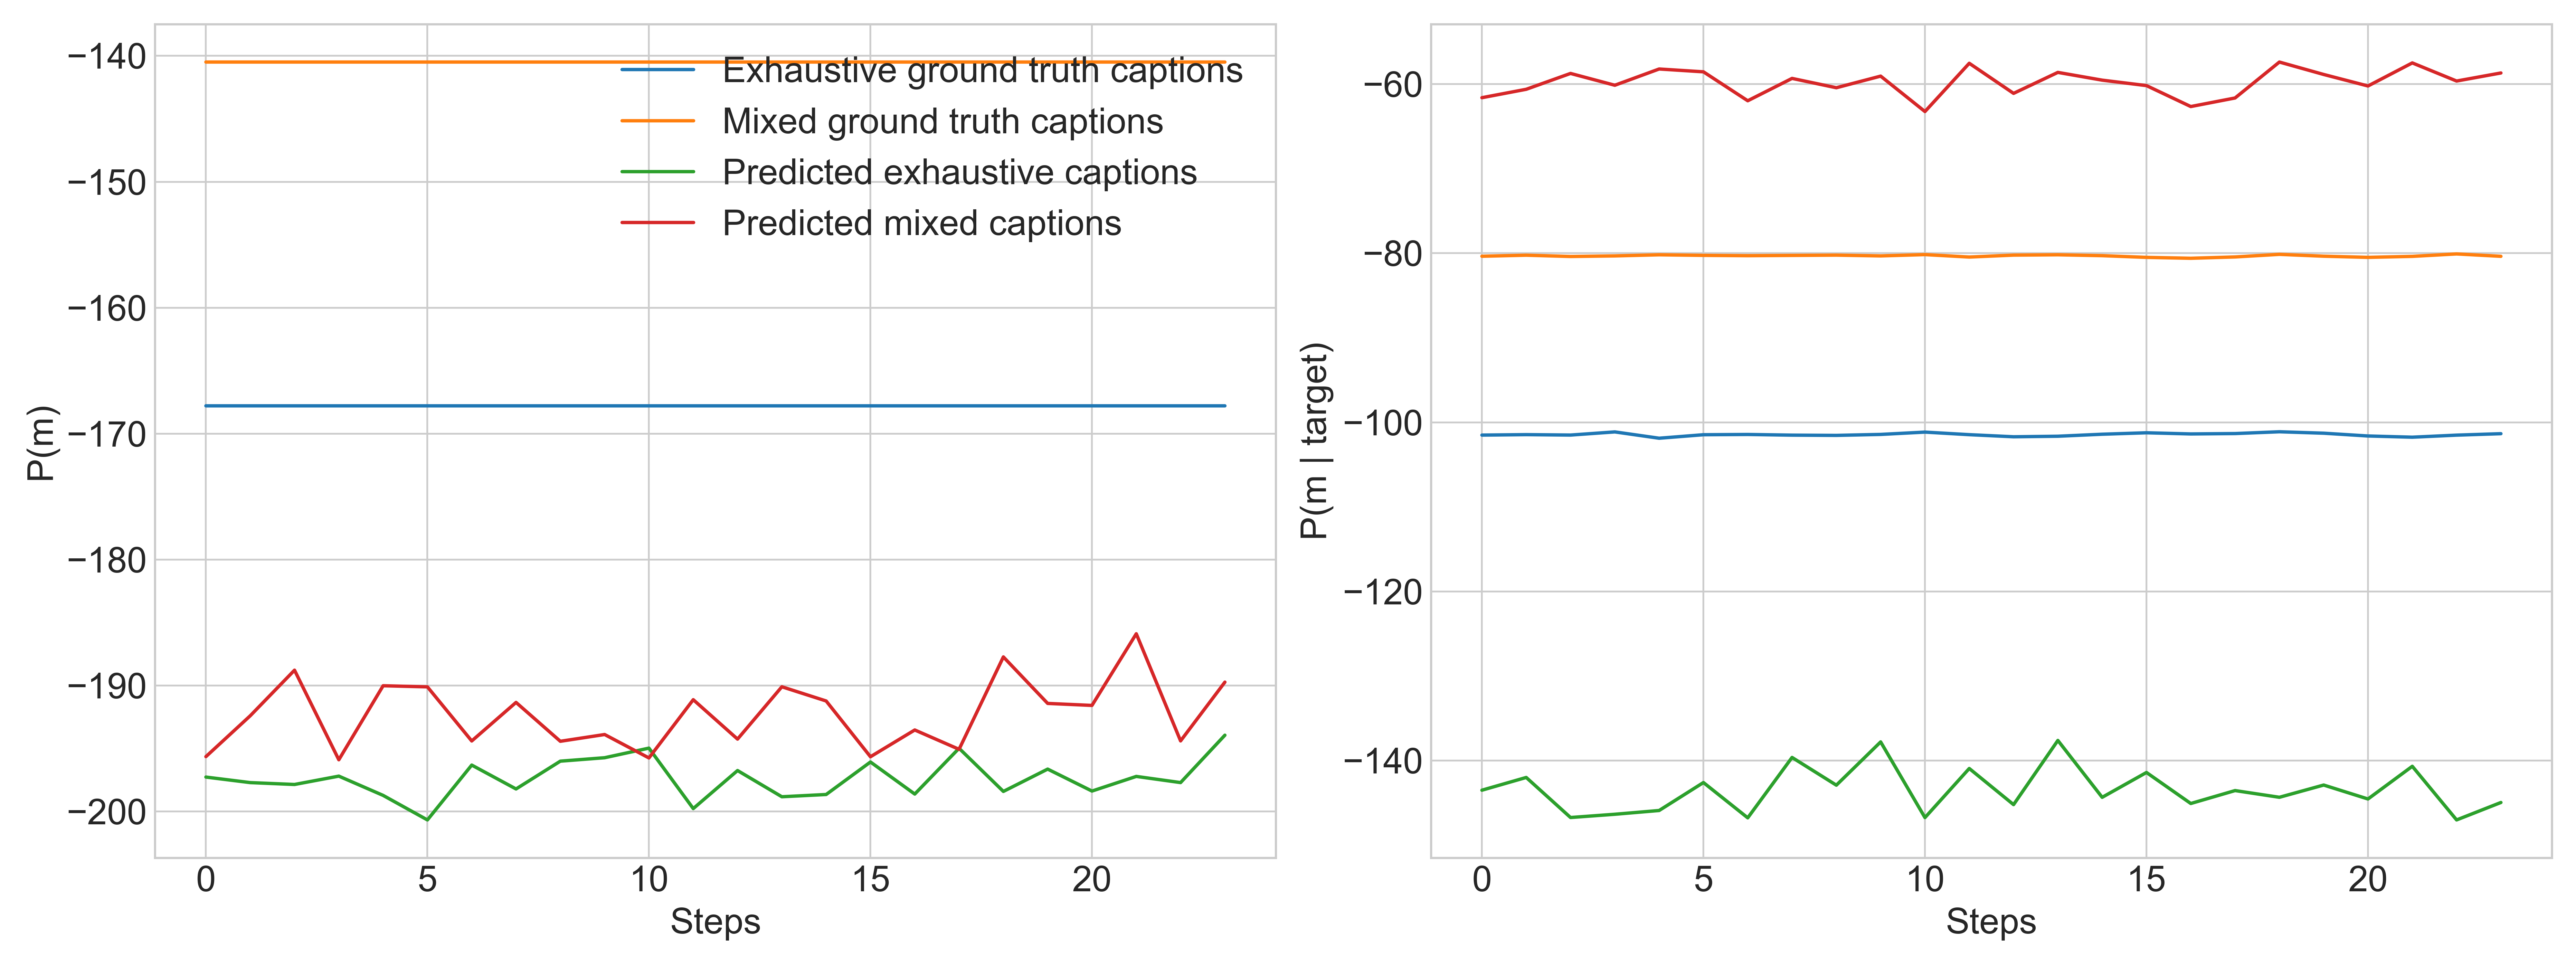
\includegraphics[width=\linewidth]{images/3dshapes_exh_short_structural_semantic_drift_49_pure_075_similarFixed.png}
	\caption{Drift dynamics computed during reference game training on both short and exhaustive captions of 3Dshapes (pure decoding, $\lambda_s=0.75$). Higher values indicate less drift. Left: Structural drift of ground truth and predicted captions under the pretrained Transformer XL model. Right: Semantic drift of ground truth and predicted captions under the pretrained speaker model.}
	\label{fig:3dshapes_wShort_similarFixed_075_str_sem_drift}
\end{figure}

\textbf{H10} and a little bit \textbf{H5}.
Baseline, similar pairs.


%\begin{figure}
%	\centering
%	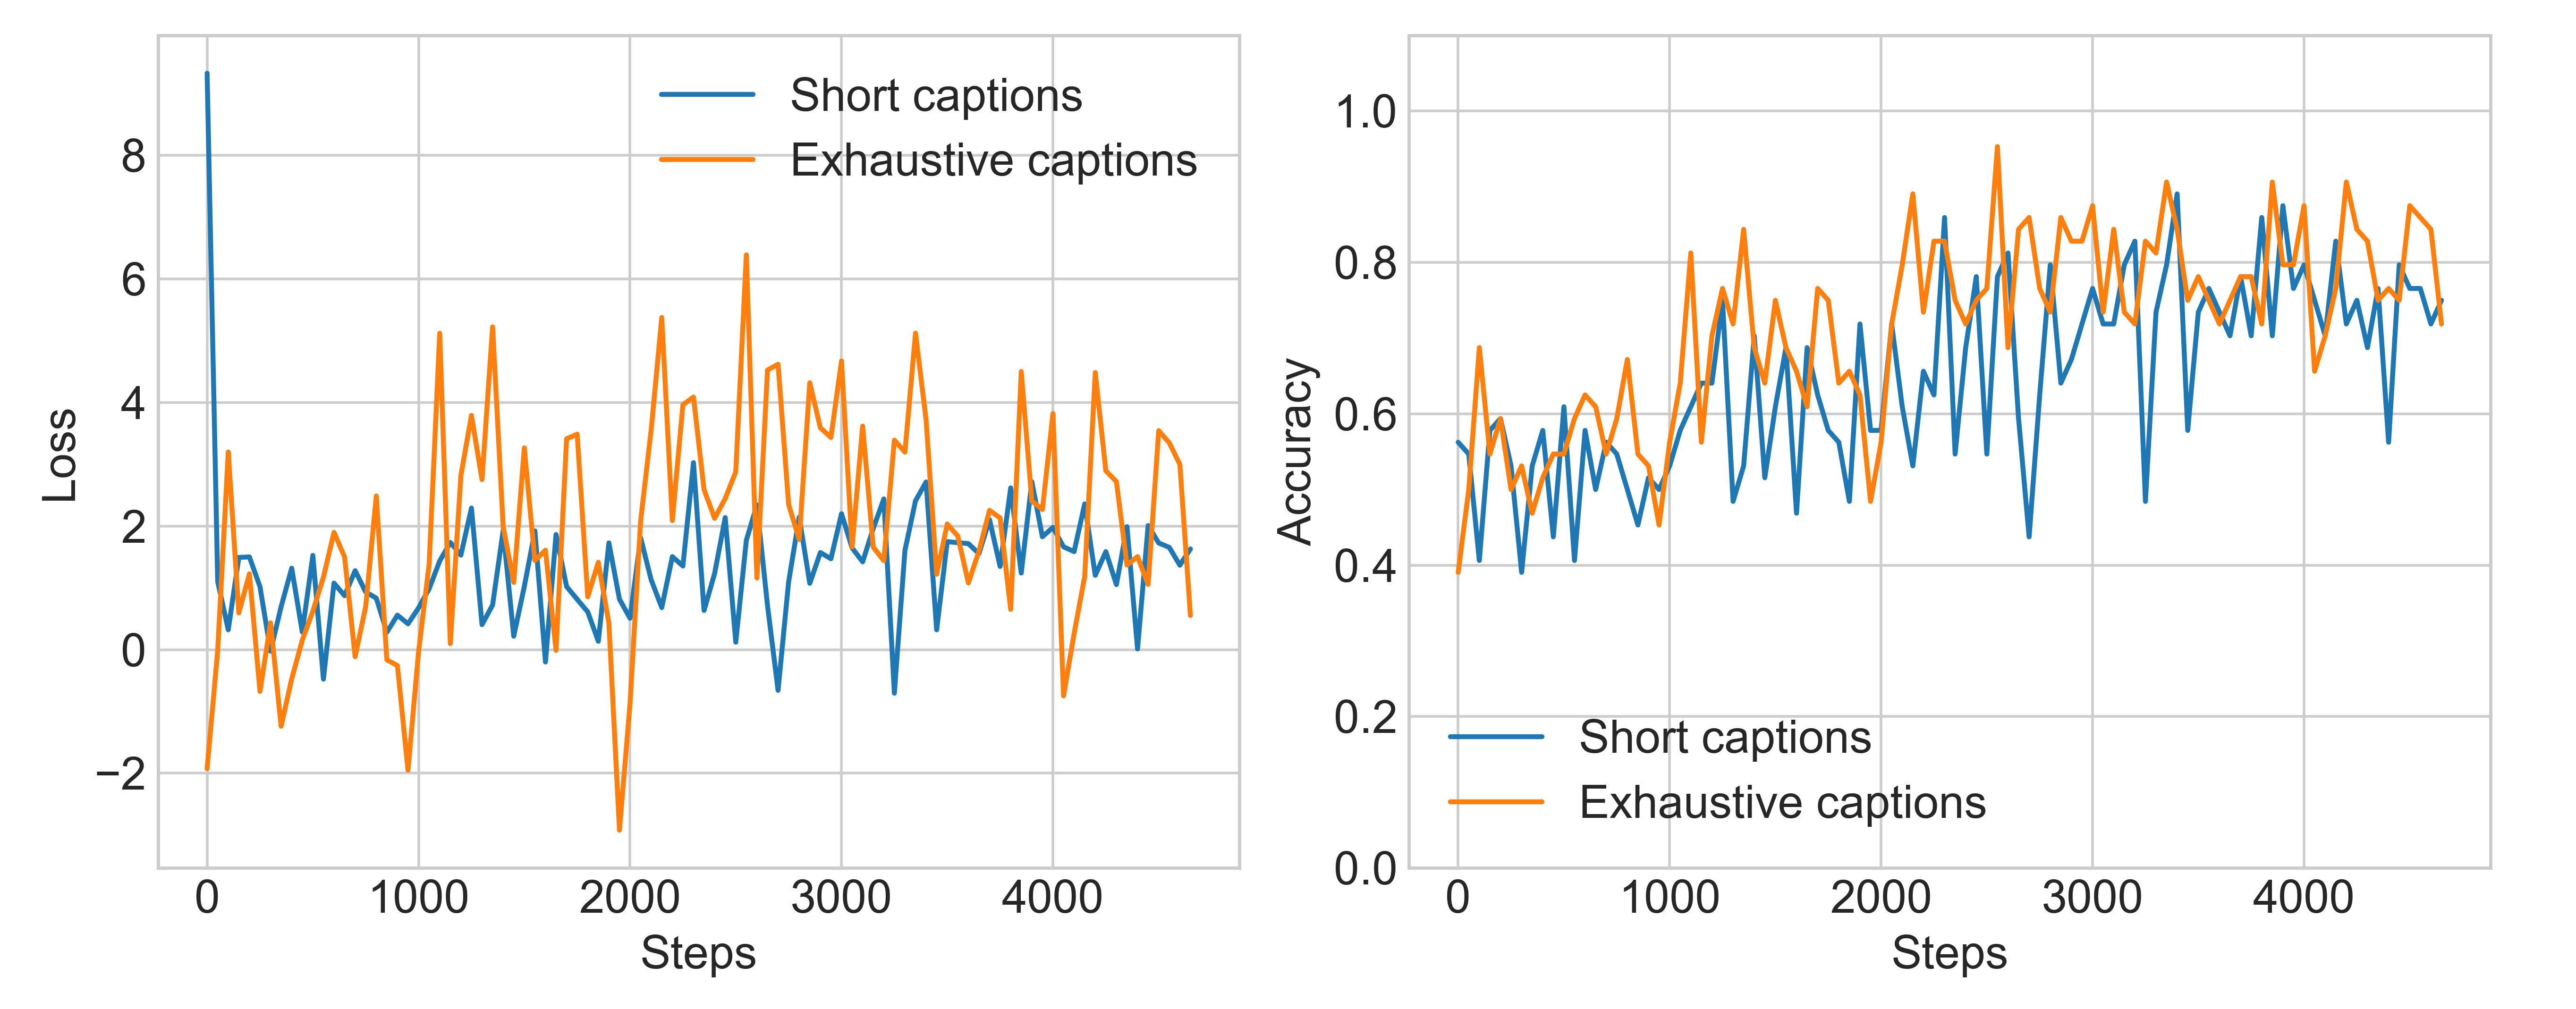
\includegraphics[width=\linewidth]{images/shapes_short_vs_exh_refgame_49_pure_075_similar.png}
%	\caption{Training dynamics on similar image pairs given a dataset with exhaustive captions vs. short captions only.}
%	\label{fig:3dshapes_short_v_exh_similar_losses}
%\end{figure}
%Given the strong effect of length, it does not come surprising that the structural drift of exhaustive captions is higher than of short ones. However, the semantic drift is much more severe for short captions, compared to exhaustive ones, therefore, at least partly supporting \textbf{H10}. 
%\begin{figure}
%	\centering
%	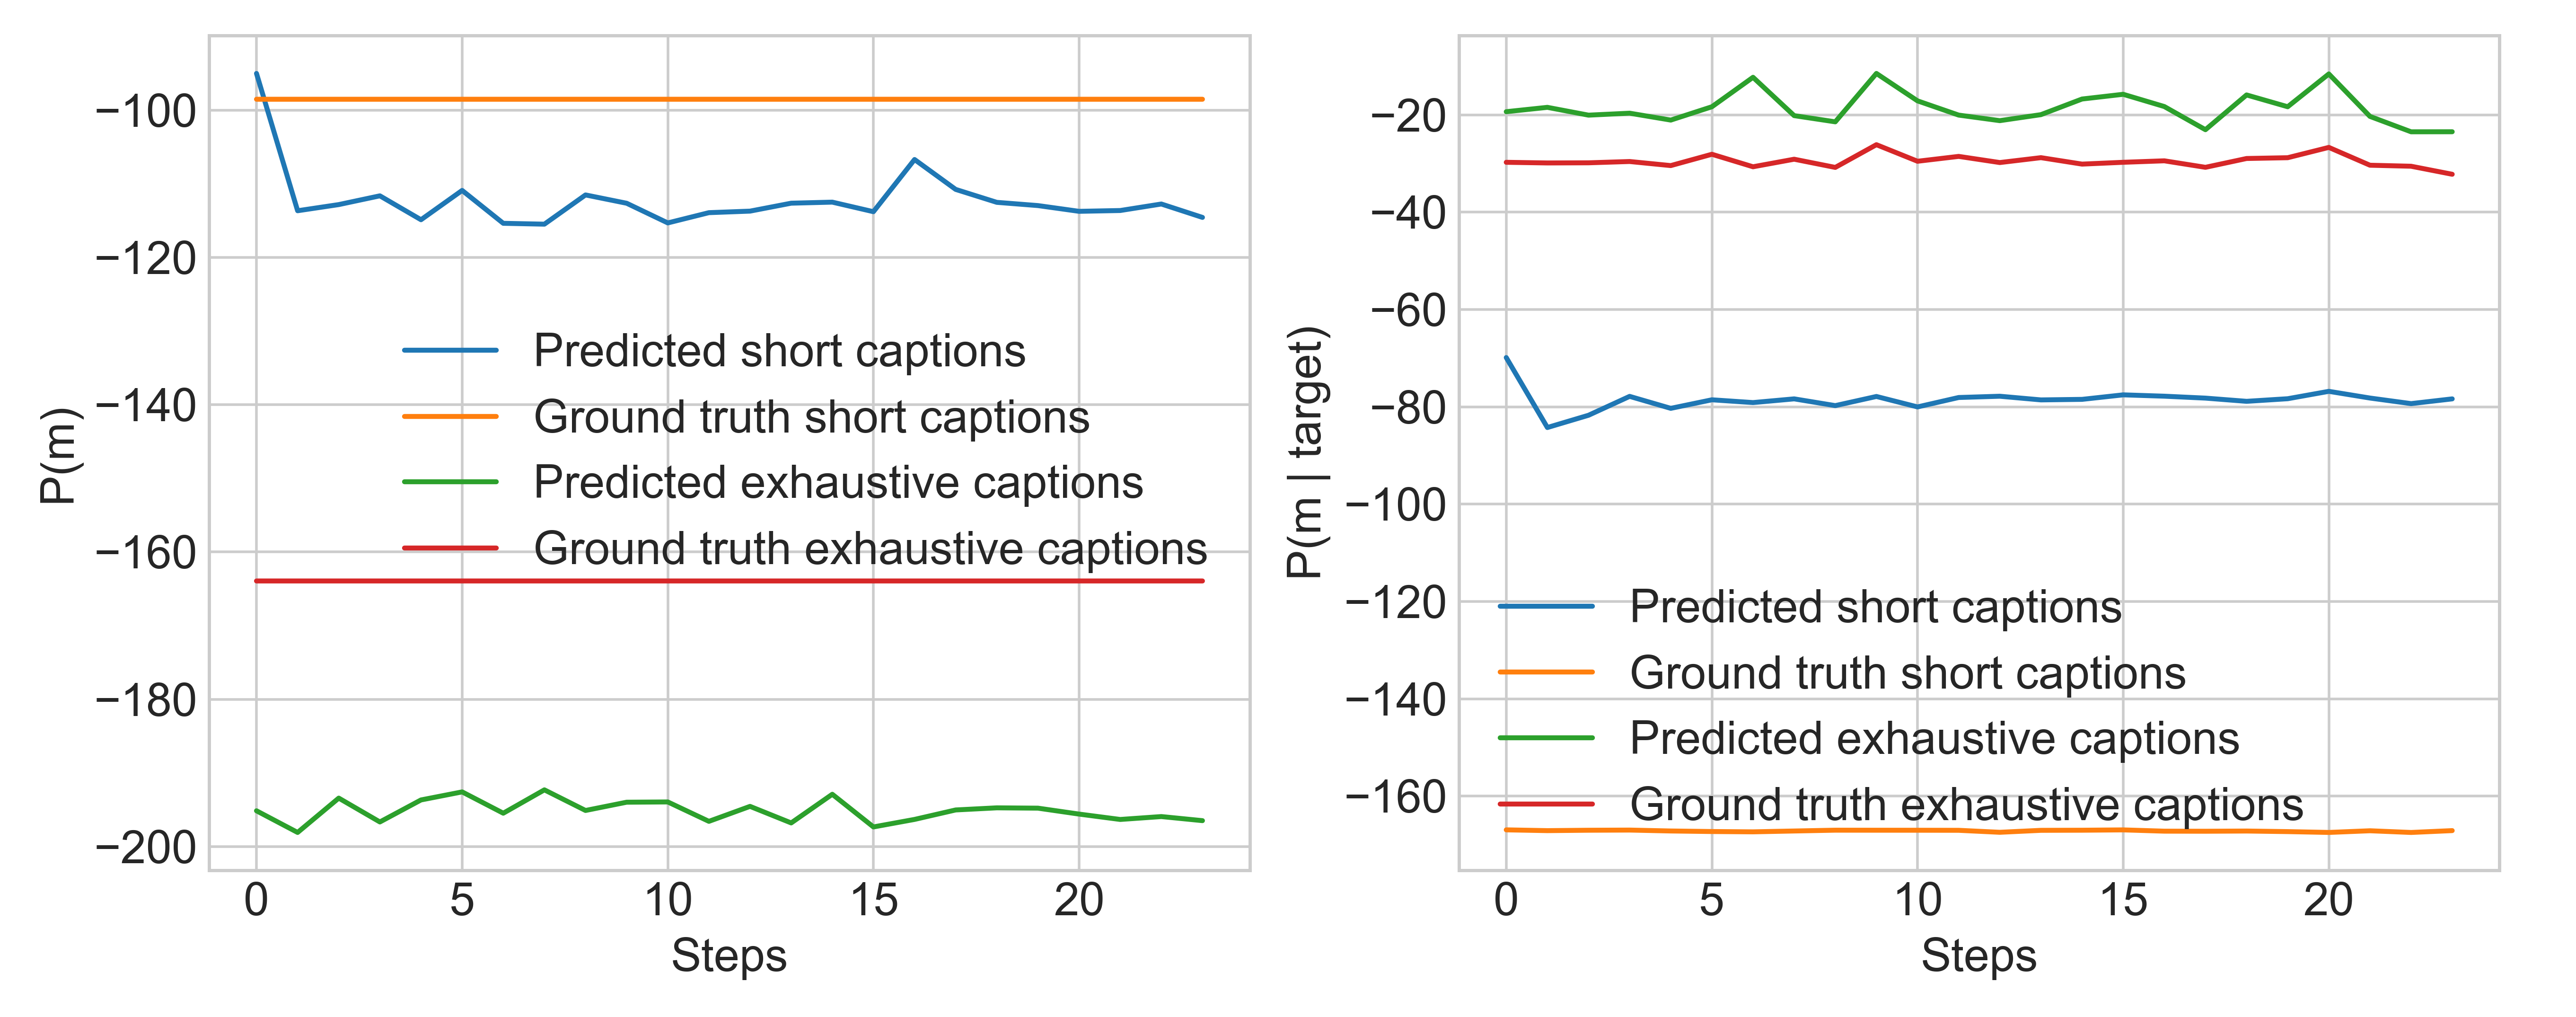
\includegraphics[width=\linewidth]{images/3dshapes_short_vs_exh_structural_semantic_drift_49_pure_075_similar.png}
%	\caption{Language drift metrics computed during training gieven model trained on similar image pairs given a dataset with exhaustive captions vs. short captions only. The drifts were computed on random image pairs for comparability.}
%	\label{fig:3dshapes_short_v_exh_similar_str_sem}
%\end{figure}


\section{Language Drift Hypotheses: Discussion}
\pt{\textbf{H9} will be discussed here (compute differences bw tuned and pretrained agent.)}

Fixed listener results consistent with \cite{lazaridou2020multi}.

Note that I did not use the term ``functional'' drift once. Add that in overlap metric discussions.

Reasons / effects behind drift: pretraining mode of agents in combination with reference game training signal; strength of functional signal (to a small extent); action space / vocabulary size. 

If there is no difference between exhaustive and short captions on 3D, it is actually promising - it means that it is not necessary to really have completely exhaustive (almost task-specific) annotations - it is sufficient that the agents saw possible descriptions of all features during pretraining, even when the sentences were short. This means, we can indeed achieve something with RL and interactive learning from experience, it is not all about supervised learning for a given task.